
\documentclass[a4paper]{article}
%\usepackage{fontspec}
\usepackage{bugtracker}
\usepackage[intlimits]{amsmath}
\usepackage{amssymb}
\usepackage{amsfonts}
\usepackage{hyperref}
    \hypersetup{pdfborder={0 0 0}}
% \usepackage{amsthm}

% Ein Haekchen aus pifont:
\usepackage{pifont}
\newcommand{\ok}{\ifmmode\text{\ding{51}}\else \ding{51}\fi}
\newcommand{\scissor}{\ifmmode\text{\ding{33}} \else \ding{33}\fi}

\declarebugtrackeritem{pgfbug}{1}
\bugtrackerset{
    prefix=bugtracker/minimal_,
}

\usepackage{todonotes}
\newcommand\todosp[2][]{%        % Stefan Pinnow
    \todo[
%        disable,
        color=blue!40,
        #1]{#2}
}

% Fix overfull hboxes automatically:
\tolerance=2000
\emergencystretch=15pt

\author{Christian Feuersänger}
\title{Todolist for PGFPlots\\\texttt{\small\pgfplotscommandtostring\pgfplotsrevision\temp\temp}}


\begin{document}
\maketitle
\tableofcontents


% =============================================================================
\section{发布待办事项}

每次发布都必须完成以下步骤：

\begin{itemize}
    \item 针对 pgf CVS 运行测试
    \item 针对最新的 pgf 稳定版运行测试
    \item 完成手册
        %
        \begin{itemize}
            \item 更新 \verb|compat| 键的说明，以记录
                \verb|pgfplots.preliminaries.tex| 中最新兼容性级别所引入的
                更改。

                注意，键 \verb|/pgfplots/compat/mostrecent| 会在手册中凡需要
                建议级别的地方自动插入。
            \item 在 \verb|\pgfplots.preamble.tex| 中禁用 \verb|\todosp|
            \item 修复警告
            \item 通览一遍
                %
            \item \verb|colorbar horizontal| 的示例使用了 ``rand''
                ——有一次它产生了意料之外的输出，且不知为何。需留意它。
        \end{itemize}
        %
    \item 确保 ``编译'' 矩阵（本列表下方）对于 pgf CVS 和最新 pgf 稳定版
        是完整的
    \item 运行 context 测试（基本上就是编译并通览一遍。没有断言。）
        %
        \begin{itemize}
            \item 针对 pgf CVS 运行
            \item 针对最新 pgf 稳定版运行
        \end{itemize}
    \item 用 "RELEASED VERSION XXX" 更新 ChangeLog，并更新 README
    \item 为新版本打上 git 标签
    \item 运行 \verb|scripts/pgfplots/pgfplotsrevisionfile.sh|，根据标签
        指定包版本 \par
        （编译手册时会自动完成）
    \item 重新编译手册（以获取正确的版本号）
    \item 运行基础示例文件
        %
    \item 调整发布 makefile 以得到正确的文件名
    \item 确保版权声明是最新的，至少在 README 中如此
    \item 打包 TDS.zip 和 CTAN.zip（使用发布 makefile）
        %
        \begin{itemize}
            \item \verb|make -f pgfplots/scripts/pgfplots/Makefile.pgfplots_release_sourceforge|
                \par
                这会生成发布文件
            \item 确保归档中不包含错误的文件。
        \end{itemize}
        %
    \item 上传到 CTAN。
        %
\begin{verbatim}
Submitted to host
    dante.ctan.org
Your name and email
    Christian Feuersänger <cfeuersaenger@users.sourceforge.net>
Filename
    pgfplots_1.6.1.ctan.flatdir.zip
Version number
    1.6.1
description:
PGFPlots draws high-quality function plots in normal or logarithmic scaling with
a user-friendly interface directly in TEX. The user supplies axis labels, legend entries
and the plot coordinates for one or more plots and pgfplots applies axis scaling,
computes any logarithms and axis ticks and draws the plots. It supports line
plots, scatter plots, piecewise constant plots, bar plots, area plots, mesh and surface
plots, patch plots, contour plots, quiver plots, histogram plots, box plots, polar axes,
ternary diagrams, smith charts and some more.

Pgfplots is based on PGF/TikZ (PGF); it runs with LaTeX/TeX/ConTeXt.
Location on CTAN
    /graphics/pgf/contrib/pgfplots/
Summary description
    pgfplots - Create normal/logarithmic plots in two and three dimensions for LaTeX.
License type
    gpl
Announcement text
    ...
Notes to maintainers
    As requested, I created a flat directory structure containing all files
    (i.e.\@ it contains latex style files, context package files, plain tex
    include files, generic implementation files, and LUA code all in the same
    directory). I will also upload a TDS zip file to
    /install/graphics/pgf/contrib/pgfplots.
    Thanks for maintaining CTAN!

\end{verbatim}
        %
        Attention: the announcement text must not be too long. In particular,
        README extracts are too long.

    \item 发布到 sourceforge。
        %
        \begin{itemize}
            \item 记得更新顶层的 README。
            \item 记得将新的 TDS 标记为 ``所有平台的默认下载''
        \end{itemize}
        %
    \item 上传到 sourceforge 网站空间（使用发布 makefile）
        %
        \begin{itemize}
            \item \verb|make -f pgfplots/scripts/pgfplots/Makefile.pgfplots_release_sourceforge uploaddist|
                这会复制手册
            \item 把 \verb|Makefile.pgfplots_release_sourceforge| 改回
                unstable
            \item \verb|make -f pgfplots/scripts/pgfplots/Makefile.pgfplots_release_sourceforge upload|
                这会更新 unstable
            \item 如有必要，更新
                \verb|scp://cfeuersaenger,pgfplots@web.sourceforge.net/htdocs/index.php|
        \end{itemize}
        %
    \item 发送公告到 \verb|pgfplots-features@lists.sourceforge.net|
    \item 使用 \verb|git push origin --tags| 或 \verb|git push origin 1.13|
        推送标签
\end{itemize}


% =============================================================================
\section{测试}

最近一次测试核验：

\begin{tabular}{lllllll}
                          & pgf git  & pgf 3.0.1 & pgf 3.0.0  & pgf 2.10  & pgf 2.00           & pgf 2.00+compat=default \\
        \hline
    回归测试             & for 1.17 & for 1.16  & for 1.12.1 & for 1.12* & for 1.8 (7\% fail) & 2009-12-30              \\
    单元测试             & for 1.16 & for 1.16  & for 1.12   & for 1.12  &                    &                         \\
    手册                 & for 1.17 & for 1.16  & for 1.12   & for 1.9   & for 1.5            &                         \\
    pgfplotstable.pdf     & for 1.17 & for 1.16  & for 1.12   & for 1.9   & for 1.5            &                         \\
    示例 latex           & for 1.16 &           &            & for 1.9   & 2009-12-30         &                         \\
    示例 context(mkII)  & for 1.15 &           &            & for 1.9   & 2009-12-30         &                         \\
    示例 context(mkIV)   & for 1.16 &           & for 1.12.1 & for 1.9   & 2009-12-30         &                         \\
    示例 plain tex       & for 1.16 &           &            & for 1.9   & 2009-12-30         &                         \\
    测试 context (mkII)  & for 1.15 &           & for 1.12   & for 1.9   &                    &                         \\
    测试 context (mkIV)  & for 1.16 &           & for 1.12*  &           &                    &                         \\
\end{tabular}

注意，context MK IV 需要把 pgfplots 安装在 \verb|~/texmf|（它不尊重环境变量）

context MK IV 可能需要一个特殊环境，例如 \verb|. ~/context/tex/setuptex|


% =============================================================================
\section{文档待办}

\begin{bugtracker}

\begin{doctodo}
    为 pgfplotstable 记录 \verb|\boldmath $...$|
\end{doctodo}

\begin{doctodo}
    scatter rgb 尚未记录
\end{doctodo}

\begin{doctodo}
    记录 standalone 与 external 的对比
    %
    \begin{itemize}
        \item standalone 无法与循环配合工作（对比
            \url{http://tex.stackexchange.com/questions/191108/how-to-avoid-copied-code-with-the-combination-pgfplots-standalone}）
        \item 使用 standalone 时，无需文档即可只生成单张图更为简单
        \item external 无缝集成
        \item external 可在之后再启用
        \item external 支持 label+ref
        \item external 开箱即用地支持 make
        \item external 支持 bounding box 控制（trim）
        \item $\cdots$
    \end{itemize}
\end{doctodo}

\begin{doctodo}
    堆叠图 + nodes near coords 的新 API 尚缺，其中包括 normalized axis cs，
    但参见 \verb|\pgfplotspointgetnormalizedcoordinates|
\end{doctodo}

\begin{doctodo}
    记录使用 lualatex 时的安装要求（LUAINPUTS 应包含 pgfplots 安装目录）
\end{doctodo}

\begin{doctodo}
    pgfplotstable 的示例 Tex 文件似乎缺了一行：
    \verb|\usepackage{pgfplotstable}|。

    此外，作为入门，若能从文件读取数据，最好再为这些数据附一个简短的
    绘图示例文件。
\end{doctodo}

\begin{doctodo}[-]
    尝试绘制一个每个柱单独着色的柱状图

    FIXME：补充细节
\end{doctodo}

\begin{doctodo}[-]
    contour：一个更改 label dist 的改动
\end{doctodo}

\begin{doctodo}[-]
    记录 'execute at begin axis' 及其新变体
\end{doctodo}

\begin{doctodo}[-]
    记录如何针对 coordindex 绘图
\end{doctodo}

\begin{doctodo}[-]
    记录如何定位 "dimension too large" 错误的来源：tracingstuff。
\end{doctodo}

\begin{doctodo}[-]
    看起来 AMS 命令 \verb|$\text{\ref{ref:to:a:plot}}$| 会把
    \verb|\ref| 实例化至少四次。想办法记录最好改用 '\verb|\hbox|'
\end{doctodo}

\begin{doctodo}[-]
    clickable 库：
        我的印象是 acroread 仅在手册上触发警告
        ——并非每次使用 clickable 库时都如此。为何！？
\end{doctodo}

% -----------------------------------------------------------------------------

\begin{doctodo}[+]
    layers（图层）：
    %
    \begin{enumerate}
        \item \ok 动机与用例
        \item \ok 简单示例
        \item \ok 多坐标轴讨论
        \item \ok tikz 集成
        \item \ok 解释如何合并自定义图层与 pgfplots 图层（并说明
            pgfplots 会覆盖 tikz 的图层）
        \item \ok 特殊之处：定义自己的图层集
        \item \ok 局限：列出受支持的锚点，并解释 cell picture 的影响
    \end{enumerate}
    %
    标记路径的裁剪应始终启用 —— 但至少对分层图形如此。它还需要更好的 UI

    TODO：
    %
    \begin{itemize}
        \item 为坐标轴路径实现 'clip mode=individual'

            FIXME：是否有充分理由说明为何 \verb|clip mode=global| 不适合
            作为默认值！？

            或许分层图形特性可以先以第一个版本发布 —— 使用
            \verb|clip mode=global|。反正它更简单。
        \item \ok 记录 'mark layer'
    \end{itemize}
\end{doctodo}

\begin{doctodo}[+]
    记录使用 lualatex 的好处（内存限制）
\end{doctodo}

\begin{doctodo}[+]
    pgfplotstable：文档化以下用法：
    &
\begin{verbatim}
\pgfplotstabletypeset[
  typeset cell/.append code={%
        \ifnum\pgfplotstablerow<0
            \pgfkeyssetvalue{/pgfplots/table/@cell content}{}%
        \fi
  },
  outfile={table},
  header=false,
  columns/0/.style={string type,column type=r},
  columns/1/.style={string type,column type=l},
  columns/2/.style={string type,column type=l}
  ]
\end{verbatim}
    %
    可用于去掉所显示的表头行。
\end{doctodo}

\begin{doctodo}[+]
    \verb|smithchart mirrored| 尚无文档！参见
    \url{https://sourceforge.net/tracker/?func=detail&atid=1060657&aid=3486928&group_id=224188}
\end{doctodo}

\begin{doctodo}[+]
    记录 \verb|axis lines=none| 本质上是 \verb|hide axis| 的别名。
\end{doctodo}

\begin{doctodo}[+]
    记录如何在绘图内部使用 decorations
    %
\begin{verbatim}
  \begin{tikzpicture}[]
    \begin{axis}[axis lines=middle,
        xmin=-2,
        xmax=2,
        ymin=-2,
        ymax=2,
        xtick={-1,1},
        ytick={-1,1},
        yticklabel=\ ,% this disables the standard tick label *text* (but not the line)
        extra description/.code={
            % this generates custom y labels to implement individual
            % styles for every tick:
            \node[below left] at (axis cs:0,-1) {$-1$};
            \node[above left] at (axis cs:0,1) {$1$};
        },
        axis line style={->},
      ]%,x=1cm,y=1cm]
      \addplot[samples=100,domain=0:2*pi,
        % tedious, but necessary: pgfplots accidentally resets the
        % "decorate" option at the beginning of the path (probably a
        % bug).
        % This is a work-around:
        every path/.style={
            postaction={decorate},
            every path/.style={},
        },
        decoration={markings,
                 mark=at position 0.25 with {\arrow{>}},
                 mark=at position 0.5 with {\arrow{>}},
                 mark=at position 0.75 with {\arrow{>}}}
        ]
        ({sin(deg(2*x))}, {sin(deg(x))});
    \end{axis}
  \end{tikzpicture}
\end{verbatim}
\end{doctodo}

\begin{doctodo}[+]
    记录关于数字格式选项的一些常见问题。\par
    其中应包含：如何为对数坐标轴得到非指数形式的数字打印
\end{doctodo}

\begin{doctodo}[+]
    \verb|\pgfplotspointplotattime|。
\end{doctodo}

\begin{doctodo}[+]
    记录通过手动提供单位向量来获得倾斜 3D 坐标轴的可能性
\end{doctodo}

\begin{doctodo}[+]
    \verb|\addplot table from| 仍受支持 —— 写一条脚注记录 ``from'' 关键字。
    %
\begin{verbatim}
  \begin{tikzpicture}
    \begin{axis}
    % All these things are valid:
            \pgfplotstableread{data-set-two.txt}\datatable
        \addplot table[y = c] {\datatable} ;
        \addplot table[y = d] \datatable ;
        \addplot table[y = a] from \datatable ;
        \addplot table[y = b] from {\datatable} ;
    \end{axis}
  \end{tikzpicture}
\end{verbatim}
\end{doctodo}

\begin{doctodo}[+]
    contour：文档在很大程度上缺失。

    缺少对 point meta 的说明。
\end{doctodo}

\begin{doctodo}[+]
    记录新的 'data cs' 特性
\end{doctodo}

\begin{doctodo}[+]
    记录如何绘制带（白色）填充单元的 mesh 图（参见 matlab 的 mesh 函数）。

    应与 surf 配合 faceted color=white 相同。
\end{doctodo}

\begin{doctodo}[+]
    记录 \verb|scale mode| 以及其他与绘图图形相关的微调
\end{doctodo}

\begin{doctodo}[+]
    改进 \verb|\pgfplotsforeachungrouped| 的文档：
    %
\begin{verbatim}
        \pgfplotsforeachungrouped \i/\j in {
            1 / a,
            2 / b,
            3 / c
        }{
    \edef\temp{\noexpand\node at (axis cs: \i,0.5) {\j};}
    % \show\temp % zum Verständnis, was als Resultat dann in \temp steht
    \temp
        }
\end{verbatim}

\begin{verbatim}
           \pgfplotsforeachungrouped \i/\j in {
            1 / a,
            2 / b,
            3 / c
        }{
    I = \i, J = \j;
        }
\end{verbatim}
\end{doctodo}

\begin{doctodo}[+]
    在 \verb|symbolic x coords| 的文档中提及 \verb|xtick=data|
\end{doctodo}

\begin{doctodo}[+]
    为 \verb|xbar| 与 \verb|ybar| 绘图处理程序提供更多示例和更详细的文档

    文档建议：依我看，最好把尺寸、分辨率以及坐标轴的对应关系描述得
    更详细一些

    示例文件：
    %
\begin{minimal}
\documentclass[a4paper]{report}
\usepackage{pgfplots}
    \pgfplotsset{compat=1.3}
\begin{document}
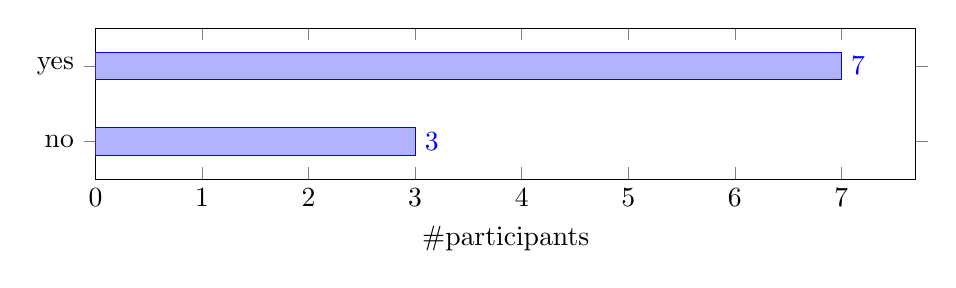
\begin{tikzpicture}
    \begin{axis}[
        xbar,
        width=12cm,
        height=3.5cm,
        enlarge y limits=0.5,
        xlabel={\#participants},
        xmin=0,
        symbolic y coords={no,yes},
        ytick=data,
        nodes near coords,
        nodes near coords align={horizontal},
    ]
        \addplot coordinates {(3,no) (7,yes)};
    \end{axis}
\end{tikzpicture}

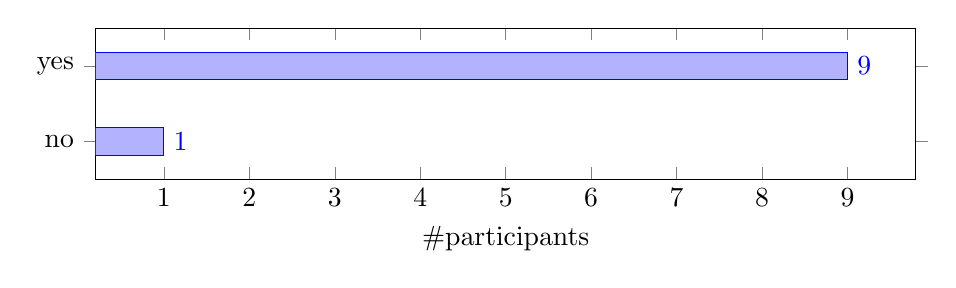
\begin{tikzpicture}
    \begin{axis}[
        xbar,
        width=12cm,
        height=3.5cm,
        enlarge y limits=0.5,
        xlabel={\#participants},
        symbolic y coords={no,yes},
        ytick=data,
        nodes near coords,
        nodes near coords align={horizontal},
    ]
        \addplot coordinates {(1,no) (9,yes)};
    \end{axis}
\end{tikzpicture}

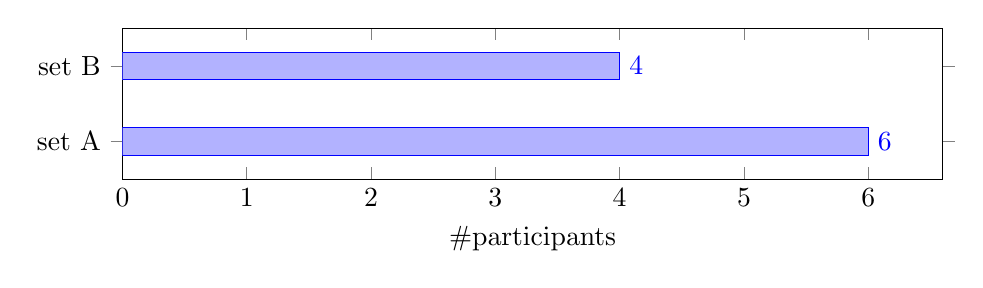
\begin{tikzpicture}
    \begin{axis}[
        xbar,
        width=12cm,
        height=3.5cm,
        enlarge y limits=0.5,
        xlabel={\#participants},
        xmin=0,
        symbolic y coords={set A,set B},
        ytick=data,
        nodes near coords,
        nodes near coords align={horizontal},
    ]
        \addplot coordinates {(6,set A) (4,set B)};
    \end{axis}
\end{tikzpicture}

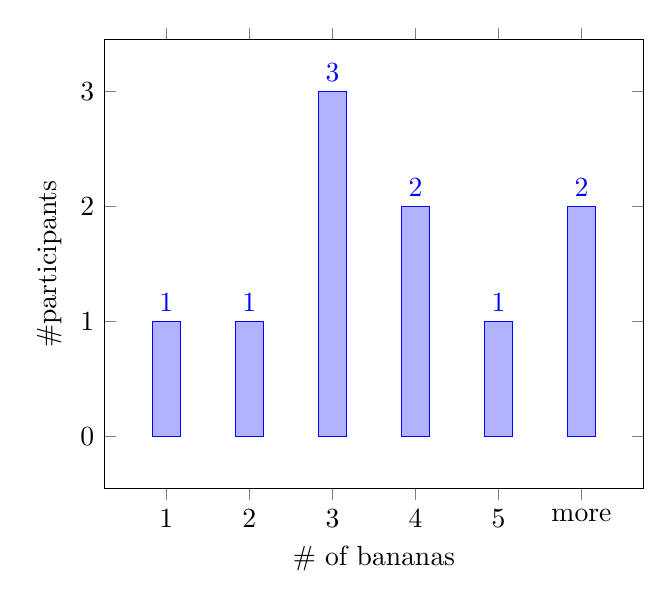
\begin{tikzpicture}
    \begin{axis}[
        ybar,
        enlargelimits=0.15,
        xlabel={\# of bananas},
        ylabel={\#participants},
        ytick={0,1,2,3},
        ymin=0,
        symbolic x coords={1,2,3,4,5,more},
        nodes near coords,
    ]
        \addplot coordinates {(1,1) (2,1) (3,3) (4,2) (5,1) (more,2)};
    \end{axis}
\end{tikzpicture}

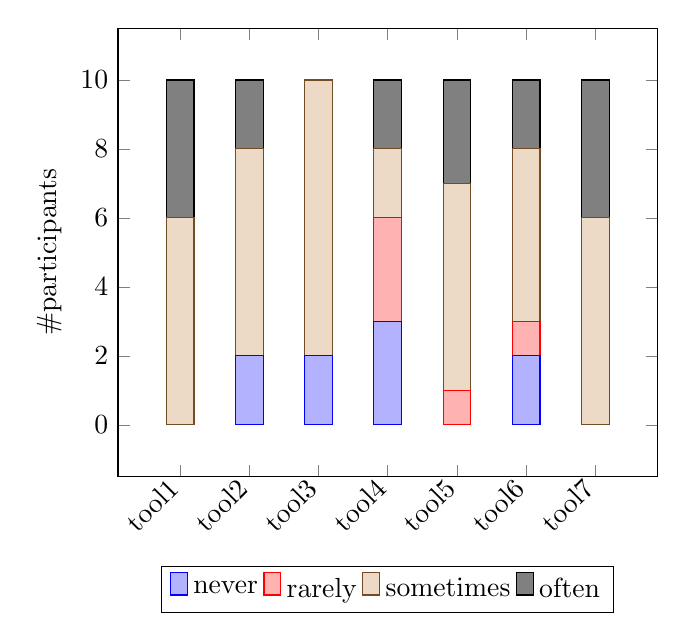
\begin{tikzpicture}
    \begin{axis}[
        ybar stacked,
        enlargelimits=0.15,
        legend style={at={(0.5,-0.20)},
          anchor=north,legend columns=-1},
        ylabel={\#participants},
        symbolic x coords={tool1, tool2, tool3, tool4, tool5, tool6, tool7},
        xtick=data,
        x tick label style={rotate=45,anchor=east},
    ]
        \addplot+[ybar] plot coordinates {(tool1,0) (tool2,2) (tool3,2) (tool4,3) (tool5,0) (tool6,2) (tool7,0)}; % never
        \addplot+[ybar] plot coordinates {(tool1,0) (tool2,0) (tool3,0) (tool4,3) (tool5,1) (tool6,1) (tool7,0)}; % rarely
        \addplot+[ybar] plot coordinates {(tool1,6) (tool2,6) (tool3,8) (tool4,2) (tool5,6) (tool6,5) (tool7,6)}; % sometimes
        \addplot+[ybar] plot coordinates {(tool1,4) (tool2,2) (tool3,0) (tool4,2) (tool5,3) (tool6,2) (tool7,4)}; % often
        \legend{never, rarely, sometimes, often}
    \end{axis}
\end{tikzpicture}

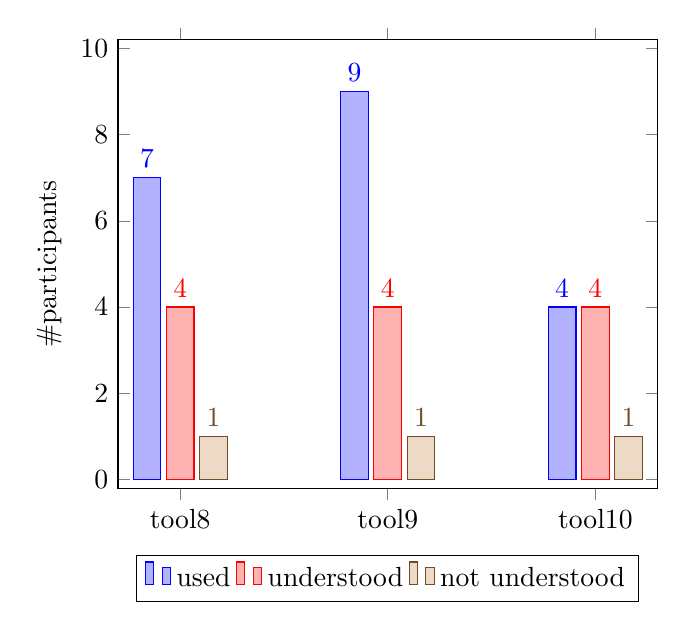
\begin{tikzpicture}
    \begin{axis}[
        ybar,
        enlargelimits=0.15,
        legend style={at={(0.5,-0.15)},
          anchor=north,legend columns=-1},
        ylabel={\#participants},
        symbolic x coords={tool8,tool9,tool10},
        xtick=data,
        nodes near coords,
        nodes near coords align={vertical},
    ]
        \addplot coordinates {(tool8,7) (tool9,9) (tool10,4)};
        \addplot coordinates {(tool8,4) (tool9,4) (tool10,4)};
        \addplot coordinates {(tool8,1) (tool9,1) (tool10,1)};
        \legend{used,understood,not understood}
    \end{axis}
\end{tikzpicture}

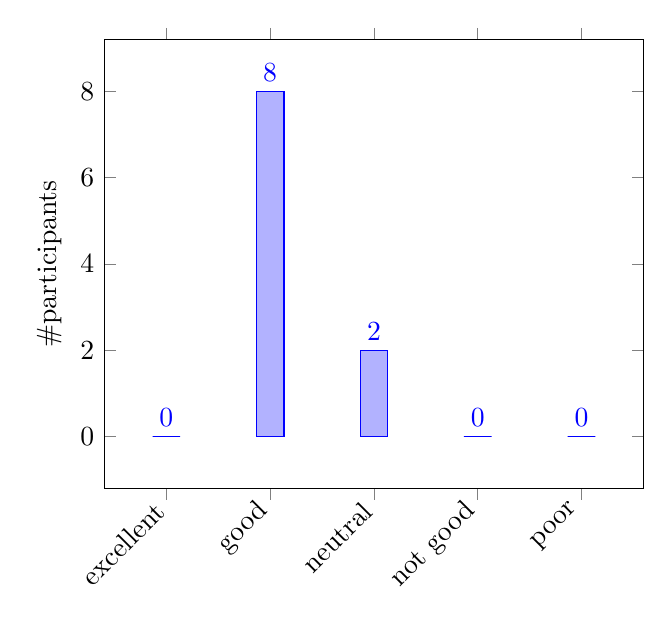
\begin{tikzpicture}
    \begin{axis}[
        ybar,
        enlargelimits=0.15,
        legend style={at={(0.5,-0.2)},
          anchor=north,legend columns=-1},
        ylabel={\#participants},
        symbolic x coords={excellent,good,neutral,not good,poor},
        xtick=data,
        nodes near coords,
        nodes near coords align={vertical},
        x tick label style={rotate=45,anchor=east},
    ]
        \addplot coordinates {(excellent,0) (good,8) (neutral,2) (not good,0) (poor,0)};
    \end{axis}
\end{tikzpicture}

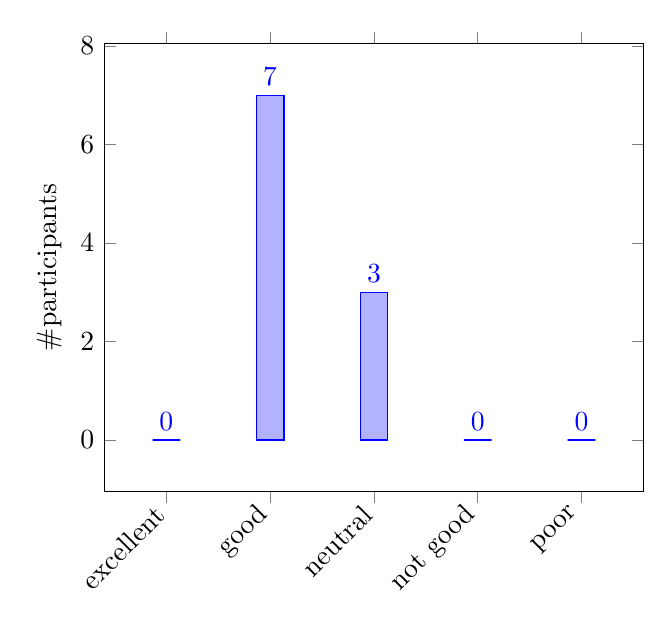
\begin{tikzpicture}
    \begin{axis}[
        ybar,
        enlargelimits=0.15,
        legend style={at={(0.5,-0.2)},
            anchor=north,legend columns=-1},
        ylabel={\#participants},
        symbolic x coords={excellent,good,neutral,not good,poor},
        xtick=data,
        nodes near coords,
        nodes near coords align={vertical},
        x tick label style={rotate=45,anchor=east},
    ]
        \addplot coordinates { (excellent,0) (good,7) (neutral,3) (not good,0) (poor,0)};
  \end{axis}
\end{tikzpicture}
\end{document}
\end{minimal}
\end{doctodo}

\begin{doctodo}[+]
    发布说明：
    提及 'shader=interp' 的改进
\end{doctodo}

\begin{doctodo}[+]
    quiver：测试里还有一个更漂亮的示例，quiver 叠加在 surf 之上，
    附着在 z=2 附近。
\end{doctodo}

\begin{doctodo}[+]
    记录 'shader=faceted interp'
\end{doctodo}

\begin{doctodo}[+]
    记录 'mesh/type'
\end{doctodo}

\begin{doctodo}[+]
    记录 'plot graphics/points' 特性。
\end{doctodo}

\begin{doctodo}[+]
    记录 'contour prepared'、'contour external' 与 'contour gnuplot'。
\end{doctodo}

\begin{doctodo}[+]
    contour external：别忘了 \verb|\", \'| 等特殊处理。
\end{doctodo}

\begin{doctodo}[+]
    contour：记录 'labels over line' 样式
\end{doctodo}

\begin{doctodo}[+]
    contour：记录对 "point meta" 的特殊处理。
\end{doctodo}

\begin{doctodo}[+]
    clickable：
        记录 'popup size' 及其变体
        记录 `clickable coords size'
        记录 'richtext' 及格式化相关内容
        记录 \verb|\n| 等
\end{doctodo}

\begin{doctodo}[+]
    记录 ternary 库
        + 别忘了 'cartesian cs' 及其应用
\end{doctodo}

\begin{doctodo}[+]
    记录 frac whole 格式
\end{doctodo}

\begin{doctodo}[+]
    记录 /pgfplots/empty line
\end{doctodo}

\begin{doctodo}[+]
    记录 'clickable coords' 与 'clickable coords code' 特性
\end{doctodo}

\begin{doctodo}[+]
    记录新的 'getcolumnbyname={create col/....}' 特性
\end{doctodo}

\begin{doctodo}[+]
    记录线性回归
\end{doctodo}

\begin{doctodo}[+]
    记录如何解决 dimension too large 问题：例如用 restrict to domain
\end{doctodo}

\begin{doctodo}[+]
    colorbar 样式在文档与代码之间不一致
\end{doctodo}

\begin{doctodo}[+]
    pgfplotstable：演示如何使用 '\verb|\begin{longtable}|'
\end{doctodo}

\end{bugtracker}


% =============================================================================
\section{PGF/TikZ 中的缺陷/特性}

\begin{bugtracker}

\begin{pgfbug}[-]
  external 缺陷：
  %
\begin{verbatim}
\documentclass[
    pagesize=auto,              % 1
        ]{scrbook}
\usepackage{tikz}
    \usetikzlibrary{external}
    \tikzexternalize
\begin{document}
    \KOMAoption{twoside}{semi}  % 2
        test
    \tikz \draw (0,0) circle (3pt);
\end{document}
\end{verbatim}

    TODOsp：我尝试了所有被注释行的组合（启用/不启用 externalization），
    结果都相同。由于你没有说明这个缺陷 \emph{如何} 表现出来，请自行复查。
    我认为：可作为已解决而关闭。
\end{pgfbug}

\begin{pgfbug}
    external 与 tcolorbox 无法协同工作
    \url{http://tex.stackexchange.com/questions/319647/tikz-package-external-causes-an-unclosed-tikzpicturetcbhooked-environment}

    TODOsp：一个已被采纳的解决方案建议使用
    \verb|\tcbset{shield externalize}| 即可解决该问题。或许，若发生错误，
    可检查是否加载了 \verb|tcolorbox|，若是，
    并提示上述方法或许有助于解决该问题？
\end{pgfbug}

\begin{pgfbug}
    自 PGF 3.0.0 起，绘图中的 topath 失效：下面应当是一条连通的线
    （就像 2.10 时那样）：
    %
\begin{verbatim}
\documentclass{standalone}
\usepackage{tikz}
\begin{document}
    \begin{tikzpicture}
        \draw (-1,-1) -- (0,0)
            -- plot [id=x,domain=0.7:1.0] function {x};
    \end{tikzpicture}
\end{document}
\end{verbatim}

    TODOsp：看起来已修复。我只得到一条线（但由于我没有 PGF 3.0.0，
    无法测试该版本下发生了什么。）
\end{pgfbug}

\begin{pgfbug}
    external 库不能正确重编译外部文件中未解析的引用，参见
    \url{http://texwelt.de/wissen/fragen/7948/markierung-in-pgfplotlegende-fehlerhaft-ubernommen?Seite=1#7973}

    TODOsp：在你回答下方的评论里有一个链接，提供了该问题可能的补丁/解决方案。
    请查看一下。
\end{pgfbug}

\begin{pgfbug}
    Beamer + pgf：默认模板会在顶部引入一条白线。
    有趣的是，它只在 PGF CVS + beamer 下出现，但似乎也依赖第三方工具
    （参见与 Stefan Tibus 的邮件往来）

    TODOsp：请至少发一封附 MWE 的邮件，看看该缺陷是否仍然存在。
\end{pgfbug}

\begin{pgfbug}
    当 externalize 函数与 transform canvas 一起使用时，结果不知为何被裁剪了。
    见本例，对比停用与启用 externalize 的输出。
    %
\begin{verbatim}
\documentclass{article}
\usepackage{tikz}
    \usetikzlibrary{external}
    \tikzexternalize % activate!
\begin{document}
    \begin{tikzpicture}[transform canvas={scale=0.7}]
        \node {root}
            child {node {left}}
            child {node {right}
            child {node {child}}
            child {node {child}}
        };
    \end{tikzpicture}
    A simple image is \tikz \fill (1,0) circle(5pt);.
\end{document}
\end{verbatim}
%
% TODOsp: still present, also with `pgfplots.external' (v1.14)
\end{pgfbug}

\begin{pgfbug}[open]
    pgf users 第 50 卷第 6 期：
    %
\begin{verbatim}
Hi,

Thanks for TikZ.  I'm trying to use the externalization library with
the class file gOMS2e.cls, which is provided for the journal
Optimization Methods and Software.  The class file and related
files/documentation can be found here:
http://www.tandf.co.uk/journals/authors/gomslatex.zip

My problem is that the externalized figures are shifted up and to the
left significantly, cutting them off.  This problem does not occur
when not using externalization.
This seems to be related to the problem discussed here:
http://sourceforge.net/tracker/index.php?func=detail&aid=3037831&group_id=142562&atid=752792
and may also be related to this one:
http://sourceforge.net/mailarchive/forum.php?thread_name=4C0F342B.5040008%40ins.uni-bonn.de&forum_name=pgf-users

In the other cases, the solution was to use \tikzifexternalizing for
whatever conflicts with the externalization, but it seems that I can't
do this when my class file is the offending bit.  Is this true?  I
would really like to be able to use the correct \documentclass to
generate the figures so that the size/fonts/etc. are consistent
throughout the resulting document.

A minimal test example is included at the end of this message.  It
appears that the image is shifted ~1.25cm to the left and ~0.8cm up.
The problem goes away when using \documentclass{article}.
I'm using the CVS version of pgf, and I get the same result when I
produce postscript figures by using latex and setting
 \tikzset{external/system call={
   latex \tikzexternalcheckshellescape -halt-on-error
-interaction=batchmode -jobname "\image" "\texsource";
   dvips -o "\image".ps "\image".dvi}}

%----------------------------------------------------------------------------------
\documentclass[printer]{gOMS2e}
\usepackage{tikz}
\usetikzlibrary{external}
\tikzexternalize
\begin{document}
\begin{center}
  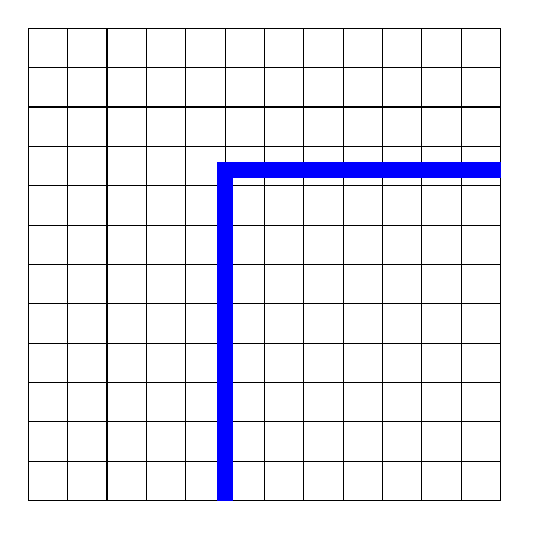
\begin{tikzpicture}
    \draw[step=.5cm] (-3,-3) grid (3,3);
    \draw[blue,line width=2mm] (-0.5,-3) -- (-0.5,1.2) -- (3,1.2);
  \end{tikzpicture}
\end{center}
\end{document}
%----------------------------------------------------------------------------------

Any help would be appreciated; I'm afraid it's over my head at this point.
Thanks!
\end{verbatim}
\end{pgfbug}

\begin{pgfbug}[-]
    考虑一种 matrix 样式，它只作用于外层 matrix 节点样式
    （参见特性请求
    \url{https://sourceforge.net/tracker/?func=detail&atid=1060657&aid=3019259&group_id=224188}）

    TODOsp：已为此创建特性请求
    \url{https://sourceforge.net/p/pgf/feature-requests/103/}
\end{pgfbug}

\begin{pgfbug}[-]
    让对 \verb|\pgf@x| 与 \verb|\pgf@y| 的赋值始终为 \verb|\global|
\end{pgfbug}

\begin{pgfbug}[-]
    实现 \verb|\pgfmathfloattocount|
\end{pgfbug}

\begin{pgfbug}[-]
    激活的 '\verb$|$' 字符会导致编译缺陷
    （\verb|\usepackage{program}|）
\end{pgfbug}

\begin{pgfbug}[-]
    用 [node font units]1em 实现 'text height=1em'
\end{pgfbug}

\begin{pgfbug}[-]
    fpu 无法在路径内部使用。应当修复。
    $\leadsto$ 问题在于路径可能直接使用 \verb|\pgfmath...| 例程。
    $\leadsto$ 这应当可行！至少用公开的数学宏 \verb|\pgfmathadd| 时应当如此。
    \verb|\pgfmathadd@| 的实现方式可能不同。
\end{pgfbug}

% -----------------------------------------------------------------------------

\begin{pgfbug}[closed]
    把 dvips 等的默认 'system call' 打包进驱动！
\end{pgfbug}

\begin{pgfbug}[closed]
    阅读手册 v2.0 时我在 5.1 "Styling the nodes" 发现一处拼写错误。
    在第一段代码之后，有一句写着
    "... can achieve them. Once way is to use ..."，应为
    "One way is to use ..."
\end{pgfbug}

\begin{pgfbug}[closed]
    某种不兼容
    %
\begin{verbatim}
\documentclass{article}
\usepackage{german}
\usepackage[utf8]{inputenc} % erlaubt direkte Nutzung von Umlauten

\usepackage{pgfplots} % für plots

\usepackage{pgfplotstable} % für Numeriktabellen
\usepackage{array,colortbl,booktabs}
\usetikzlibrary{external}
\tikzexternalize[force remake]

% DOESN'T WORK. Needs to disable externalization
\usepackage{vmargin}
\setpapersize{A4}
\setmarginsrb{2.5cm}{1cm}{2cm}{2cm}{8mm}{15mm}{5mm}{15mm}

\begin{document}
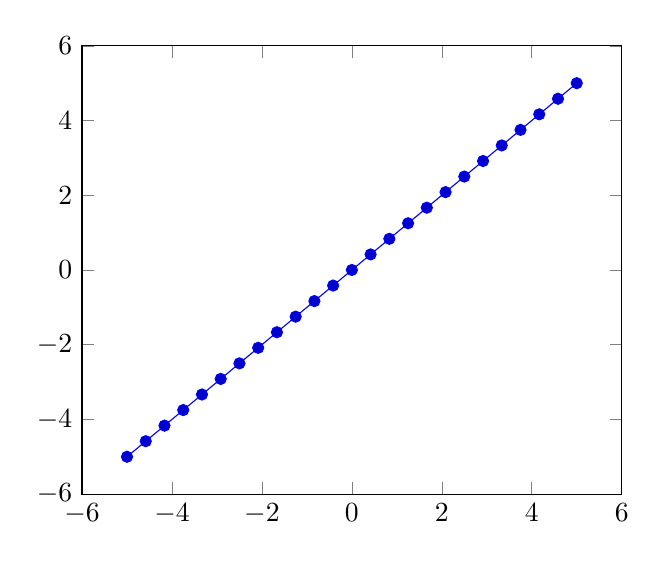
\begin{tikzpicture}
%\tracingmacros=2 \tracingcommands=2
    \begin{axis}
        \addplot {x};
    \end{axis}
\end{tikzpicture}
\end{document}
\end{verbatim}
\end{pgfbug}

\begin{pgfbug}[closed]
    若使用 \verb|\cite[][]{dd}|，external 库会失败，参见 MWE 及变通方法
    \url{http://tex.stackexchange.com/questions/173465/tikz-error-for-externalized-graphics-but-output-is-correct/178684#178684}
\end{pgfbug}

\begin{pgfbug}[closed]
    用 lualatex 运行时，external 库不能正确为子进程计算 shell escape 标志。

    此外，最好能自动检测 lualatex 驱动。
\end{pgfbug}

\begin{pgfbug}[+]
    数字打印机：把
    \verb|set thousands separator={\cdot}| 同样应用到小数部分：
    %
\begin{minimal}
\documentclass{article}
\usepackage{pgf}
    \pgfset{/pgf/number format/.cd,
        set thousands separator={{{\cdot}}},
        precision=5,
    }
\begin{document}
    \pgfmathprintnumber{12345.54321}      \par
    $12 \cdot 2345.543 \cdot 21$ expected \par
\end{document}
\end{minimal}
\end{pgfbug}

\begin{pgfbug}[closed]
    \verb|\pgfmathdivide@{-0.8}{1.00002}\pgfmathresult| 得到

    \makeatletter
    \pgfmathdivide@{-0.8}{1.00002}\pgfmathresult

    而不是 -0.8
\end{pgfbug}

\begin{pgfbug}[+]
    在 \verb|\usetikzlibrary| 及其变体中支持去除空格与空条目
\end{pgfbug}

\begin{pgfbug}[+]
    external 库：思考是否能在无需用户显式输入的情况下提供真实 jobname。
    思路：把它作为 TeX 代码参数传给 pdflatex
\end{pgfbug}

\begin{pgfbug}[+]
    为数字打印机提供 '$\times$' 或更通用的格式规则
\end{pgfbug}

\begin{pgfbug}[+]
    参数之间有空格时，code 2 args 不能正确工作！？
\end{pgfbug}

\begin{pgfbug}[+]
  external 库：实现 \verb|\tikzpicturedependsonfile#1|
\end{pgfbug}

\begin{pgfbug}[+]
    在 pgfplots 中：调用 \verb|\tikzpicturedependsonfile|。
    或许 plot-from-table 结构也应使用它。
\end{pgfbug}

\begin{pgfbug}[+]
    external 库：'list and make' 无法与 \verb|\include|（aux 文件！）
    或其他写文件操作协同工作 —— 至少在并行处理时不行。
\end{pgfbug}

\begin{pgfbug}[+]
    考虑 Andy Schlaikjer 的 "plot function" 补丁
\end{pgfbug}

\begin{pgfbug}[+]
    看起来 fadings 与 externalization 配合时不能正确工作！？
\end{pgfbug}

\begin{pgfbug}[+]
    纳入 Christophe Jorssen 为 external 库提供 MD5 校验和的补充
\end{pgfbug}

\begin{pgfbug}[+]
    编写新的子包 'pgfmanual.sty'，它为手册的样式、环境等提供良好的用户界面。
\end{pgfbug}

\begin{pgfbug}[+]
    external 库：图内的 catcode 更改不能正确工作。
\end{pgfbug}

\begin{pgfbug}[+]
    在手册中，pgfqkeysactivatesinglefamilyandfilteroptions 的前两个参数
    被写反了。
\end{pgfbug}

\begin{pgfbug}[+]
    某些预定义过滤器不能正确处理未知选项
\end{pgfbug}

\begin{pgfbug}[+]
    pgf 中的 external 库：思考 'empty image extension' 究竟是缺陷还是特性。
    $\leadsto$ 对 \verb|\pgfimage| 而言是特性！否则就无法提供扩展名！
    $\leadsto$ 对 external 库而言是缺陷，因为它从不使用扩展名！
\end{pgfbug}

\begin{pgfbug}[closed]
    修复 external 库（PGF）中的横向页面缺陷（pdflscape）
    %
\begin{minimal}
    \pdfcompresslevel=0
\documentclass{article}
\usepackage{pgfplots}
%\usepackage{lscape}
\usepackage{pdflscape}

\usetikzlibrary{external}
    \tikzexternalize

\begin{document}
\begin{landscape}
La.
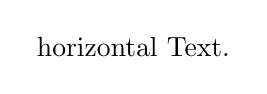
\begin{tikzpicture}
    \node at (0,0) {horizontal Text.};
\end{tikzpicture}
\end{landscape}

\end{document}
\end{minimal}
\end{pgfbug}

\begin{pgfbug}[+]
    pgf 数学解析器对 '-' 前缀运算符的优先级处理错误：
    \verb|exp(-x^2)| 是错的。
\end{pgfbug}

\begin{pgfbug}[+]
    兼容性代码待办：
        - plot graphics 的示例（带 view=0{90}）不能工作。
        $\leadsto$ 那是 '\verb|exp(0-x^2)|' 缺陷，仍存在于 pgf 2.00！
\end{pgfbug}

\end{bugtracker}


% =============================================================================
% BUGS
\section{PGFPlots 中的缺陷}

\begin{bugtracker}

\begin{bug}[prio=1]
    \verb|mark list| 会产生大量
    %
\begin{verbatim}
\XC@edef #1#2->\begingroup \ifnum \catcode `\!=13 \edef !{\string !}\fi \ifnum \catcode `\:=13 \edef :{\string :}\fi \ifnum \catcode `\-=13 \edef -{\string -}\fi \ifnum \catcode `\+=13 \edef +{\string +}\fi \ifnum \catcode `\;=13 \edef ;{\string ;}\fi \ifnum \catcode `\"=13 \edef "{\string "}\fi \ifnum \catcode `\>=13 \edef >{\string >}\fi \edef #1{#2}\@onelevel@sanitize #1\aftergroupdef #1#1
[........]
{\if}

\@@tmp ->.!80!black
{true}
{the character !}
Missing character: There is no ! in font nullfont!
{the character 8}
Missing character: There is no 8 in font nullfont!
{the character 0}
Missing character: There is no 0 in font nullfont!
{the character !}
Missing character: There is no ! in font nullfont!
{the character b}
Missing character: There is no b in font nullfont!
{the character l}
Missing character: There is no l in font nullfont!
{the character a}
Missing character: There is no a in font nullfont!
{the character c}
Missing character: There is no c in font nullfont!
{the character k}
Missing character: There is no k in font nullfont!
{\def}
{\else}
\end{verbatim}
    %
    缺陷。或许在更新版本的 xcolor 中已修复？

    TODOsp：使用 ``xcolor 2016/05/11 v2.12'' 时它仍然存在。

    你确定这是由 `xcolor' 引起的吗？这些信息似乎是由
    \verb|mark list fill| 值中的 \verb|.| 引起的。若提供一个不含点的值，
    这些信息就不会出现。

    若你确定这能在 `xcolor' 中解决，请告诉我，我会联系相应的作者求助。
\end{bug}

\begin{bug}[open,epic=units]
    在对 x SI 前缀使用预设键（milli）之后，我接下来想切回正常模式，
    于是简单地写 x SI prefix=none，遗憾的是 'none' 值未定义，
    编译无法继续
    %
\begin{verbatim}
\documentclass[border=5pt]{standalone}
\usepackage{pgfplots}
    \usetikzlibrary{pgfplots.units}
\begin{document}
    \begin{tikzpicture}
        \begin{axis}[
            change x base,
%            x SI prefix=kilo,   % <-- using this works fine
            x SI prefix=none,   % <-- using this causes the error:
            x unit=m,           %     Choice 'milli' unknown in choice key
            y SI prefix=milli,  %     '/pgfplots/x SI prefix'
            y unit=N,           %                ^ (why x and not y where 'milli' is used?)
            xlabel=Distance,
            ylabel=Force,
        ]
            \addplot coordinates {
                (1000,1)
                (2000,1.1)
                (3000,1.2)
                (4000,1.3)
            };
        \end{axis}
    \end{tikzpicture}
\end{document}
\end{verbatim}
\end{bug}

\begin{bug}[epic=polar]
    当只显示部分范围时，极坐标图不显示所有刻度线，
    参见 Christian 的回答
    \url{http://tex.stackexchange.com/questions/323462/can-one-generate-a-boxed-polar-plot-with-pgfplots-and-polaraxis/326741#326741}
\end{bug}

\begin{bug}
    1.14 中的回归：point meta 数字格式采用内部 FPU 表示，
    不再是标准数字
    \url{http://tex.stackexchange.com/questions/317365/colorbar-with-definite-number-of-discrete-colours-with-matching-ticks-placement/325584#325584}
    %
\begin{verbatim}
\documentclass[tikz,border=3pt]{standalone}
\usepackage{pgfplots}
    \pgfplotsset{compat=1.14}
\usepackage{expl3}
\ExplSyntaxOn
%%%%%%%%%%%%%%%%%%%%%%%%%%%%%%%%%%%%%%%%%%%%%%%%%%
% \fpEval{<expression>}
% expandably evaluate floating point <expression>
\let\fpEval\fp_eval:n
%%%%%%%%%%%%%%%%%%%%%%%%%%%%%%%%%%%%%%%%%%%%%%%%%%
\ExplSyntaxOff

\begin{document}
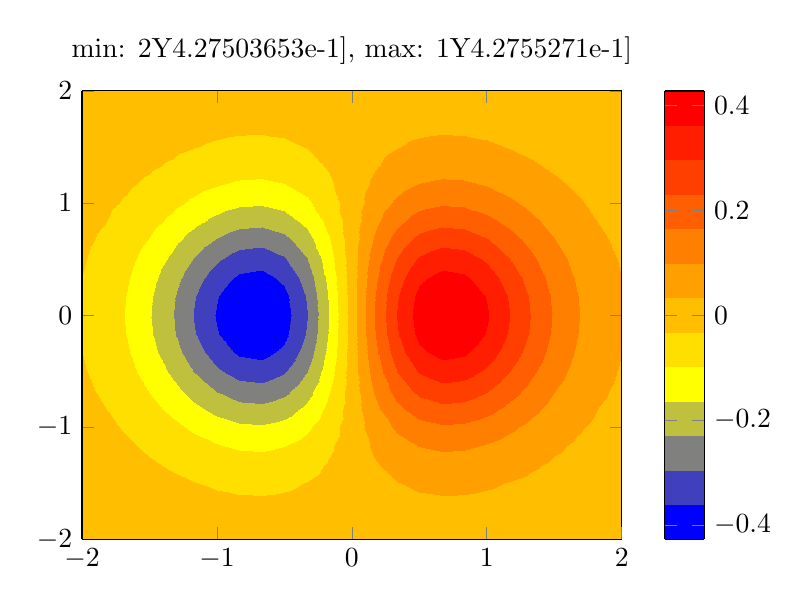
\begin{tikzpicture}
\begin{axis}[
  title={min: \pgfkeysvalueof{/pgfplots/point meta min}, max: \pgfkeysvalueof{/pgfplots/point meta max}},
  domain=-2:2,
  view={0}{90},
  colormap={CM}{
  samples of colormap=(13 of hot)},
  colormap access=piecewise constant,
  colorbar right,
% nachfolgende Berechnungen gehen nicht mehr:
%  colorbar style={%
%     ytick={%
%       \fpEval{\pgfkeysvalueof{/pgfplots/point meta min}},%
%       \fpEval{\pgfkeysvalueof{/pgfplots/point meta min}+(\pgfkeysvalueof{/pgfplots/point meta max}-\pgfkeysvalueof{/pgfplots/point meta min})/13},%
%       ...,%
%       \fpEval{\pgfkeysvalueof{/pgfplots/point meta max}*2} %increase limit to ensure placement of uppermost tick label
%     }
%  }
]
\addplot3[surf,shader=interp]
{exp(-x^2-y^2)*x};
\end{axis}
\end{tikzpicture}
\end{document}
\end{verbatim}
\end{bug}

\begin{bug}
    看起来图层配置并未真正起作用：
    \verb|set layers={axis on top}| 的效果与 \verb|axis on top| 不同。

    看起来在绘制各个实体时，我需要在某处使用 \verb|\pgfplotsgetlayerforstyle|
    —— 仅设置 \verb|on layer| 并不够。
\end{bug}

\begin{bug}[epic=fillbetween]
    fillbetween / intersection 库缺陷：
    见最小示例
    \url{http://tex.stackexchange.com/a/181224/95441}

    TODOsp：这是否与 \url{https://sourceforge.net/p/pgfplots/bugs/111/}/ 相关？
    （我也在那里记了一笔，说明它列在此处。）若 \emph{确}有相关，请删去此处条目，
    以免重复。
\end{bug}

\begin{bug}
    external 缺陷：external 库必须保留 pgfpictureid，否则它会混淆
    已记录的位置！

    MWE 见
    \url{http://tex.stackexchange.com/questions/72781/problem-tikz-pgfplots-and-external-coordinates-using-overlay/72804#comment782265_72804}

    TODOsp：现在修复了吗？至少在默认 `mode' 下，有无 externalization 没有差别。\\
    给 SP 的备注：$\to$ 再用 `mode=list and make' 检查！

    我用 1.14-74-g5452a45 仍能复现
\end{bug}

\begin{bug}
    fpu 无法计算 \verb|exp(-4.08893e7)|（在某处溢出）。

    待办：将其替换为 0
\end{bug}


\begin{bug}
    以合适的方式记录
    \url{http://tex.stackexchange.com/questions/65045/pgfplots-axis-xmode-ymode-in-user-defined-style/65069?noredirect=1#comment721421_65069}

% TODOsp: Or provide an example how it works in the manual or link to that answer ;-)
\end{bug}

\begin{bug}
    external 库把 prefix 选项搞乱了？
    \url{http://tex.stackexchange.com/questions/243935/error-using-tikz-externalize-cant-write-md5-file}
\end{bug}

\begin{bug}
    pgfmathparse 不再与 calc 宏包的 heightof 等兼容？
    \url{http://tex.stackexchange.com/questions/289551/how-to-resolve-conflict-between-versions-of-texlive-and-pgf}
\end{bug}

\begin{bug}
    colormap access=piecewise constant 会产生视觉瑕疵：
%
\begin{verbatim}
\documentclass{standalone}
\usepackage{pgfplots}
    \usepgfplotslibrary{colorbrewer}
    \pgfplotsset{compat=1.14,lua debug}
\begin{document}
\begin{tikzpicture}
    \begin{axis}[
        view={0}{90},
        colormap/Purples-6,
        colorbar,
        colormap access=piecewise constant,
    ]
    \addplot3[surf,shader=interp,] {x*y^2};
    \end{axis}
\end{tikzpicture}
\end{document}
\end{verbatim}
    %
    它正中间有一处瑕疵。Acrobat reader 与 xpdf 相比瑕疵略有不同
\end{bug}

\begin{bug}
    axis description 样式包含 ``on layer''，但它们忽略了它！
\end{bug}

\begin{bug}
    语法高亮问题：
    %
\begin{verbatim}
\begin{quote}
    |edge node=node [every edge quotes,|\meta{options}|]{|\meta{text}|}|
\end{quote}
\end{verbatim}
    %
    结果是
    %
\begin{verbatim}
    edge node=node [every edge quotes] options ]{ text }
\end{verbatim}
\end{bug}

\begin{bug}
    tikz 缺陷：使用 \verb| -- cycle| 会交换节点的起点/终点位置
        \todosp{已注释的最小示例}
%%%%%\begin{minimal}
%%%%%\documentclass{standalone}
%%%%%\usepackage{tikz}
%%%%%\begin{document}
%%%%%
%%%%%\begin{tikzpicture}
%%%%%    \fill[
%%%%%         fill opacity=0.75,
%%%%%         draw=orange!80!black,thick,
%%%%%         fill=orange,
%%%%%    ]
%%%%%    (0,1) -- (1,2) -- (2,1)
%%%%%       |- (0,0) -- cycle
%%%%%                node [coordinate,at start,pin=above right:at start] {}
%%%%%                node [coordinate,at end,pin=above left:at end] {}
%%%%%    ;
%%%%%\end{tikzpicture}
%%%%%\end{document}
%%%%%\end{minimal}
\end{bug}

\begin{bug}[epic=z buffer]
    z buffer=sort 似乎导致错误结果 —— 必须用 min(depths) 而非
    mean(depths)！
    \url{http://tex.stackexchange.com/questions/281953/perspective-error-in-pgfplots-surface}
\end{bug}

\begin{bug}
    若有人使用自定义 \verb|column type| 或 \verb|assign column name|，
    dec sep align 便不能工作。

    见
    \url{http://tex.stackexchange.com/questions/276395/pgfplotstable-formatting-problems/277284#277284}
\end{bug}

\begin{bug}
    在把映射后的坐标发送给 TeX 之前，为 lua 后端加入健全性检查：
    \url{http://tex.stackexchange.com/questions/269656/pgfplots-with-big-data-dimension-too-large}
\end{bug}

\begin{bug}
    使用 \verb|\thisrow{col}| 仅展开为该值，但不会在值周围隐式加括号。

    因此，像 \verb|\thisrow{col}^2| 这样的写法，对 $-2$ 之类的行会产生
    意料之外的结果
    \url{http://tex.stackexchange.com/questions/262774/pgfmath-misbehaving-when-reading-negative-values-from-table-in-pgfplots}

    不过，文本列仍应照常处理。另外：过去写
    \verb|\dimen0=\thisrow{col}pt| 是可行的，若自动加括号则会破坏它。

    思路：类似
    %
\begin{verbatim}
\def\thisrow#1{-2}
\let\thisrowX=\thisrow
\def\thisrow#1{(\thisrowX{#1})}%
\edef\XXX{\thisrow{col}^2}
\message{EXPANDED: \XXX^^J}
\end{verbatim}
    %
    在计算表格表达式之前？
\end{bug}

\begin{bug}[epic=precision]
    确定次刻度时不准确？
    \url{http://tex.stackexchange.com/questions/262662/pgfplots-sometimes-minor-ticks-dont-show}
    与下一个工单相关
\end{bug}

\begin{bug}[epic=precision]
    刻度标签受 Tikz foreach 中不精确算术之害：

    TODOsp：这是否与前一个缺陷同根？
    $\to$ 合并它们
    %
\begin{verbatim}
KAPUTT:

  \foreach \x in {1,1.1,...,2} {\x\par}

OK:

  \foreach \x in {1,1.1,...,2.001} {\x\par}
\end{verbatim}
\end{bug}

\begin{bug}[epic=precision]
    \verb|...| 与舍入：

    在我看来，\verb|...| 语法并不稳健。在一些小而并不罕见的区间上，
    会出现舍入误差：

    主网格：

    \verb|ytick={0.99,1.00,1.01,1.02,1.03,1.04,1.05,1.06,1.07,1.08}|

    辅助网格：

    \verb|minor ytick={0.99,0.991,...,1.08}|

    这导致辅助线随数值增大而越来越偏离主网格线，尽管它们本应重合。
    若把辅助网格完整写出：

    \verb|minor ytick={0.99,0.991,0.992,0.993,...............,1.08}|

    就正常了。因此 \verb|...| 语法绝对要慎用。

    TODOsp：这是否与前一个缺陷同根？
    $\to$ 合并它们
\end{bug}

\begin{bug}[epic=v2]
    考虑把 \verb|unbounded coords=jump| 作为 mesh/surface 图的默认。
    \url{http://tex.stackexchange.com/questions/259012/glitch-in-3d-surface-plot-using-pgfplots-not-solved-by-z-buffer}

    TODOsp：为 v2 提的特性？是（epic=v2）。
\end{bug}

\begin{bug}
    fpu 缺陷：
    %
\begin{verbatim}
\begingroup
\tracingmacros=2 \tracingcommands=2
\pgfkeys{/pgf/fpu}
\pgfmathparse{exp(-3.4814e4)}\pgfmathresult
\endgroup
\end{verbatim}
    %
    无法编译。
    \url{http://tex.stackexchange.com/questions/251496/fermi-dirac-in-pgfplots-dimension-too-lage}
\end{bug}

\begin{bug}[epic=z buffer]
    view dir=reverse 似乎会导致错误的 3D 观察方向并破坏 z 缓冲，对比
    \url{http://tex.stackexchange.com/questions/250825/axis-dir-reverse-and-colormap-bug-in-tikz}
\end{bug}

\begin{bug}
    3D 坐标轴与 y dir = reverse 似乎会破坏 z 排序，见
    \url{http://texwelt.de/wissen/fragen/6131/pgfplots-3d-oberflachenproblem}

    TODOsp：这与前一个缺陷是同一个，对吧？
    $\to$ 合并为一条
\end{bug}

\begin{bug}[epic=smithchart]
    smithchart 导纳图符号错误
    %
\begin{verbatim}
This Mail is in German, since your name suggests, that you speak German.
If that is not the case, please let me know, and I will write send you
this mail again in English.

Sehr geehrter Herr Feuersänger,

ich schreibe momentan meine Bachelor-Arbeit und muss dafür Antennen
vermessen und die Messergebnisse graphisch darstellen. Ich habe mit
Begeisterung festgestellt, dass ich mit PGFPlot recht direkt s1p- und
s2p-Dateien plotten kann.
Vielen Dank dafür!

Allerdings gibt es ein paar Darstellungsprobleme:

-> Bei Admitanzgraphen, also smithchart mirrored=true werden die
Koordinaten auf dem unteren Halbkreis mit negativen Vorzeichen
dargestellt (dies ist auch in dem Beispiel im Manual so)
Jedoch sind bei jedem Admitanz-Smith-Graph die Vorzeichen umgekehrt (da
der Admitanz-Graph per Definition 1/Z_L=1/(a+b*i)=a/(a^2+b^2)-ib/(a^2+b^2)

Gibt es eine Option das einzurichten?
    y dir=reverse
bewirkt nichts.
\end{verbatim}
\end{bug}

\begin{bug}[epic=smithchart]
    smithchart：-> 从 14cm 大小起，yticklabel around circle、
    few smithchart ticks 等就不能用了。这可手动实现：
    %
\begin{verbatim}

    \begin{smithchart}[
        title=\text{title},
        smithchart mirrored=true,
        xticklabel shift=-19pt,
        grid style={blue},
        ticklabel style={blue},
        width=15.2cm,
        xtick={0.2,0.5,1,2,5},
        ytick={0,0.2,0.5,1,2,5,-0.2,-0.5,-1,-2,-5},
        xgrid each nth passes y={2},
        ygrid each nth passes x={2},%ytick align=center,
        ytick align=center,
        yticklabel style={
            rotate=180,
        },
    ]
\end{verbatim}
\end{bug}

\begin{bug}[prio=10,epic=fillbetween]
    fill between 无法与 PGF 2.10 配合工作

    变通方法：使用以下补丁
    %
\begin{verbatim}
\documentclass[10pt]{beamer}
\usepackage{tikz}
\usepackage{pgf}
\usepackage{pgfplots}
    \usepgfplotslibrary{fillbetween}
\makeatletter
\def\tikz@intersect@addto@path@names#1#2{%
  \edef\tikz@marshal{#2\expandafter\noexpand\csname tikz@intersect@path@name@#1\endcsname}%
  \expandafter\expandafter\expandafter\def\expandafter\expandafter\expandafter\tikz@marshal%
    \expandafter\expandafter\expandafter{\expandafter\tikz@marshal\expandafter{\tikz@intersect@temppath}}%
  \expandafter\pgfutil@g@addto@macro\expandafter\tikz@intersect@namedpaths\expandafter{\tikz@marshal}%
}
\pgfkeys{%
  /tikz/name path global/.code={%
    \expandafter\global\expandafter\let\csname tikz@intersect@path@name@#1\endcsname=\relax
      \tikz@key@name@path@new{#1}{\gdef}%
  },
  /tikz/name path local/.code={%
    \pgfkeys{/tikz/name path={#1}}%
  },
  /tikz/name path/.code={%
      \tikz@key@name@path@new{#1}{\def}%
  },
}
\makeatother


\begin{document}
\begin{frame}

\begin{tikzpicture}
\begin{axis}[%
axis x line*=bottom,
ymin=0,
ymax=1,
]

\addplot[name path=h,domain=-0.01:1,blue,line width=2pt] {5.5*x^4 - 8.4*x^3 + 3.2*x^2 + 0.5*x + 0.2};
\path[name path=axis] (axis cs:0,0) -- (axis cs:1,0);

\only<2->{
\addplot [fill=green, fill opacity=0.2]
    fill between[of=h and axis, soft clip={domain=0.0:0.4}];
}

\end{axis}
\end{tikzpicture}
\end{frame}
\end{document}
\end{verbatim}
\end{bug}

\begin{bug}[prio=2,epic=lua]
    下面这段用 lualatex 无法编译（显然是因为双引号）。它在 pdflatex 下可行。

    优先级低，因为 point meta 实际并未被使用 —— 而若正确使用，
    它在 lualatex 与 pdflatex 下都可行
    %
\begin{verbatim}
\documentclass{standalone}
\usepackage{pgfplots}
    \pgfplotsset{%
        compat=newest,
    }
\begin{document}
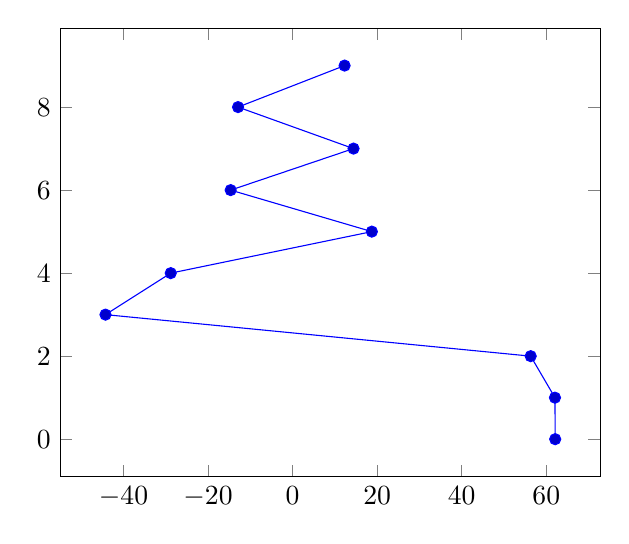
\begin{tikzpicture}
\begin{axis}[
    %point meta=explicit symbolic,
    %nodes near coords=\pgfplotspointmeta,
]
\addplot table[x index={1}, y expr=\coordindex, header=false, meta index={0}] {
"i"  62.099
"i"  62.046
"i"  56.304
"i" -44.258
"2" -28.826
"i"  18.740
"i" -14.653
"i"  14.402
"i" -12.907
"i"  12.295
};
\end{axis}
\end{tikzpicture}
\end{document}
\end{verbatim}
\end{bug}

\begin{bug}[epic=substitute axis cs,epic=smithchart]
    substitute axis cs 与 smithchart 配合时失败：
    %
\begin{verbatim}
\documentclass{standalone}
\usepackage{pgfplots}
    \usepgfplotslibrary{smithchart}
    \pgfplotsset{compat=newest}
\begin{document}
   \begin{tikzpicture}
     \begin{smithchart}
%     \pgfplotsset{is smithchart cs}
%     \begin{scope}[/pgfplots/is smithchart cs]
       \draw [black!40,dashed] (0,0) arc (0:360:.5);
%     \end{scope}
     \end{smithchart}
   \end{tikzpicture}
\end{document}
\end{verbatim}
\end{bug}

\begin{bug}[epic=substitute axis cs]
    substitute axis cs 与 \verb|++ (0,1cm)| 配合时不能工作
    （很可能每次 \verb|++| 都是如此）

    变通方法：使用 \verb|++ (0cm,1cm)| 或 \verb|compat=1.10|。
    %
\begin{verbatim}
\documentclass{article}
\usepackage{pgfplots}
\begin{document}
    \pgfplotsset{compat=1.9}
\begin{tikzpicture}
\begin{axis}[
    xmin=-1,xmax=1,
    ymin=-1,ymax=1
]
    \draw (axis cs:0,0) -- ++(0,1cm);
\end{axis}
\end{tikzpicture}

    \pgfplotsset{compat=1.12}
\begin{tikzpicture}
\begin{axis}[
    xmin=-1,xmax=1,
    ymin=-1,ymax=1
]
    \draw (axis cs:0,0) -- ++(0,1cm);
\end{axis}
\end{tikzpicture}
\end{document}
\end{verbatim}
\end{bug}

\begin{bug}[epic=fillbetween]
    error bars 与 fill between 无法协同工作（据 Jerzy Wrobel 2015 年 1 月 28 日
    的邮件）：
    %
% TODOsp: {
% - commented some hopefully not needed packages
% - data file is missing, so I cannot test, if the issue is still there
% }
\begin{verbatim}
\documentclass[12pt,border=8pt]{standalone}
%\usepackage[utf8]{inputenc}
%\usepackage{mathtools}
\usepackage{pgfplots}
%\usepackage[T1]{fontenc}
%\usepackage{fouriernc}
    \pgfplotsset{
        compat=newest,
        every axis/.append style={line width=0.03cm,axis line style={line width=0.02cm}},
        every tick/.append style={line width=0.02cm,color=black},
        every axis label/.append style={font=\small},
        tick label style={font=\small},
        legend style={font=\small,draw=none},
        title style={font=\small},
        axis on top=false,
        table/col sep=comma,
    }
    \tikzset{
        every pin/.style={font=\small},
    }
    \pgfkeys{/pgf/number format/set thousands separator = }
    \usepgfplotslibrary{fillbetween}
    \usetikzlibrary{patterns}
\begin{document}
\begin{tikzpicture}
\begin{axis}[
    width=70mm,
    height=70mm,
    axis x line=box,
    axis y line=box,
    scale only axis,
    enlarge x limits=true,
    enlarge y limits=true,
    grid=none,
    xlabel=wave length (microns),
    ylabel=Experiment1916 (a.u.),
    extra y ticks={0},
    extra y tick labels={},
    extra y tick style={
        grid=major,major grid style={line width=0.02cm,color=black,densely dashed},
    },
]
\addplot+ [
    name path=1,
    line join=round,
    every mark/.append style={solid,fill opacity=1.0},
    mark repeat=1,
    mark phase=1,
    error bars/.cd,
    y dir=both,
    y fixed=10,
] table [
    skip first n=4,
    x index=0,
    y index=1,
] {Coblentz1919.csv} ;
\path[name path=B] (0.4,0) -- (0.75,0);
\addplot[pattern=north west lines,forget plot] fill between[of=1 and B];
\end{axis}
\end{tikzpicture}
\end{document}
file:

#Spectral energy distribution of a cylindrical acetylene flame.
# T = 2360 K
# W. W. Coblentz, Scientific Papers of the Bureau of Standards, Vol.15, 639 (1920).
wave length (microns),Experiment1916 (a.u.),Revised1919 (a.u.)
0.400,5.9,5
.425,8.2,7
.440,10.0,8.5
.450,11.5,10.0
.460,13.0,11.8
.475,16.0,15.0
.500,21.9,20.9
.520,27.9,27.5
.525,29.5,29.2
.540,35.0,34.6
.550,38.9,38.9
.560,42.9,42.9
.575,49.8,49.8
.580,52.2,52.2
0.600,62.1,62.5
.620,73.0,73.3
.625,75.7,76.1
.640,84.7,85.0
.650,91.1,91.2
.660,97.4,97.6
.675,107.5,107.5
.680,110.9,110.9
.700,124.6,124.1
.720,138.5,137.5
.725,141.9,141.0
.740,152.0,151.0
.750,158.9,157.9
\end{verbatim}
\end{bug}

\begin{bug}
    使用 group plots 与间断点时出现虚假的偏移/位移：
    \url{http://tex.stackexchange.com/questions/183399/wrong-placement-and-or-size-of-picture-plot-with-groupplot-of-table-and}
\end{bug}

\begin{bug}
    去掉这个布尔量 ``apply@datatrafo@''。它是 ``is linear'' 的同义词。
    我甚至会说：把该变换也应用到对数坐标轴上，或许配一个 no-op 配置。
\end{bug}

\begin{bug}
    回归：
    %
\begin{verbatim}
\documentclass{article}
\usepackage{pgfplots}
    \pgfplotsset{compat=newest}
\begin{document}
\begin{tikzpicture}
    \begin{axis}[ybar,
        symbolic x coords={foo,bar,baz},
        x=2cm,
        enlarge x limits={abs=bar}, xtick=data,
    ]
        \addplot coordinates { (foo,1) (bar,3) (baz,2) };
    \end{axis}
\end{tikzpicture}
\end{document}
\end{verbatim}
    %
    在 1.6（正常）与 1.7（编译错误）之间的某个版本坏了。

    问题在于 \verb|\pgfkeysdef{/pgfplots/@enlargelimits/abs value}| 的定义，
    它试图判断参数是否含单位。若是，则跳过标准坐标映射器。本例中
    'abs=bar' 没有单位，但数学解析器会失败，因为该参数根本不是数学表达式……
    我该如何修复！？
\end{bug}

\begin{bug}[-,prio=1]
    interrupt bounding box 特性仍应更新数据 bounding box。
    否则，变换可能失败。
\end{bug}

\begin{bug}[epic=dateplot]
    dateplot 与 x tick label as interval 组合不能很好地协同：
    %
    \begin{itemize}
        \item 只能格式化其中一个日期
        \item 说明文字作用于\emph{右}端而非左端
    \end{itemize}

        \todosp{已注释的最小示例，因为 TeX 时会报错}
%%%%%\begin{minimal}
%%%%%\documentclass{standalone}
%%%%%\usepackage{pgfplots}
%%%%%\pgfplotsset{compat=newest}
%%%%%\usepgfplotslibrary{dateplot}
%%%%%\begin{document}
%%%%%\begin{tikzpicture}
%%%%%\begin{axis}[
%%%%%const plot, % unrelated but makes more sense of the plot
%%%%%date coordinates in=x,
%%%%%xtick=data,
%%%%%xticklabel style={rotate=90,anchor=near xticklabel},
%%%%%x tick label as interval,
%%%%%xticklabel=\tick -- \nexttick,
%%%%%]
%%%%%\addplot coordinates {
%%%%%(2009-01-01, 050)
%%%%%(2009-02-01, 100)
%%%%%(2009-03-01, 100)
%%%%%(2009-04-01, 100)
%%%%%(2009-05-01, 040)
%%%%%(2009-06-01, 020)
%%%%%(2009-07-01, 000)
%%%%%(2009-08-01, 035)
%%%%%};
%%%%%\end{axis}
%%%%%\end{tikzpicture}
%%%%%\end{document}
%%%%%\end{minimal}
\end{bug}

\begin{bug}
    xtick 键仍依赖 PGF 基础级别的 foreach —— 其中的数字似乎并未被解析。
\end{bug}

\begin{bug}[prio=3]
    TikZ 在点求值（即形如 \verb|(1,2)| 的表达式）时浪费时间：
    它调用 \verb|tikz@checkunit| 来检查单位，却把数学结果丢弃
    （之后又重新计算一遍）。
\end{bug}

\begin{bug}[epic=fillbetween]
    fillbetween + softclip：若输入路径完全落在 soft clip 区域内，
    soft clip 应直接返回输入路径。

    见
    \url{http://tex.stackexchange.com/questions/195678/pgfplots-using-the-fillbetween-library/195697?noredirect=1#comment453086_195697}

    TODOsp：这是否与 \url{https://sourceforge.net/p/pgfplots/bugs/111/}/ 相关，
    还是该缺陷另有根源？
\end{bug}

\begin{bug}
    extra ticks 会导致标签出现不期望的位移
    %
\begin{verbatim}
\documentclass[border=5pt,varwidth]{standalone}
\usepackage{pgfplots}
    \pgfplotsset{compat=newest}
\begin{document}

I'm using pgfplots 1.10 and observe the following problem. The x label
shifts down a bit if I introduce extra x ticks, even if their labels are
empty. The following example produces the observed behavior:

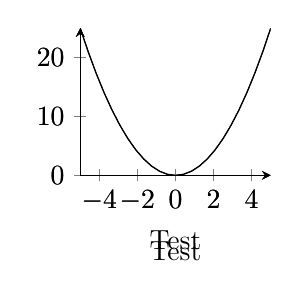
\begin{tikzpicture}
\begin{axis}[
  width=4cm,
  xlabel=Test,
  axis x line=bottom,
  axis y line=left,
]
\addplot [black] {x^2};
\end{axis}
\begin{axis}[
  width=4cm,
  xlabel=Test,
  axis x line=bottom,
  axis y line=left,
  extra x ticks={0},
  extra x tick labels={},
]
\addplot [black] {x^2};
\end{axis}
\end{tikzpicture}

It does not happen with the old, static, label placement (e.g. if I
remove the compat setting). I was not able to test with 1.11, but
there's nothing related mentioned in the release notes, if I did not
overlook it. Any ideas what I'm missing or if it is a bug and how to
work around it? I need two adjacent graphs in subfloats but only one of
them has extra ticks, so the spacing should be equal to look reasonable.
Adding an extra tick on the other plot helps, but the spacing looks
better without, so that's not an option. And switching back to the old
behavior means manually tweaking the distance, what makes no sense to me
either.

\end{document}
\end{verbatim}
    %
    根源：\verb|\pgfplots@ticklabel@maxtickdimen@finish| 被调用了两次：
    一次用于普通刻度，一次用于 extra ticks（注意 \verb|*reset| 例程只调用一次）。
    然而 \verb|@finish| 例程会加入一些 \verb|@extrashift| —— 这也做了两次。
    额外偏移属于刻度偏移。
\end{bug}

\begin{bug}
    组合绘图处理程序（hist、boxplot、contour）在其首次 survey 阶段需要访问
    坐标过滤器等。
\end{bug}

\begin{bug}[prio=3]
    contour 绘图处理程序不允许 'name path'。
\end{bug}

\begin{bug}[prio=1]
    contour 绘图处理程序不允许分别指定 draw 与 fill —— 若只绘制/填充
    一条等值线，这会很有用。
\end{bug}

\begin{bug}
    pgfplots 无法处理对数图上非常小的数值范围
    （即 xmin 与 xmax 彼此非常非常接近时）。

    见
    \url{http://www.mrunix.de/forums/showthread.php?76399-tikz-PGFplots-Fehler-dimension-too-large&p=358818#post358818}
%
% TODOsp: I am sure that I have seen this on TeX.SX as well ...
\end{bug}

\begin{bug}[epic=nodes near coords]
    ybar interval 与 nodes near coords 不能很好地配合

    ybar interval 有一个人为的末坐标。它也会收到 nodes near coords。

    见
    \url{http://tex.stackexchange.com/questions/181061/pgfplots-clipping-everything-outside-a-specific-area}
\end{bug}

\begin{bug}[epic=nodes near coords]
    ybar interval + nodes nears coords：节点发生位移。

    此处该偏移不起作用。

    See
    \url{http://tex.stackexchange.com/questions/181061/pgfplots-clipping-everything-outside-a-specific-area}
\end{bug}

\begin{bug}
    坐标过滤 + error bars 不能工作。

    预期行为：应先计算误差坐标，再把坐标过滤器应用到结果上。目前，过滤器先被
    求值，然后是误差坐标。

    见
    \url{http://tex.stackexchange.com/questions/154084/how-to-scale-both-data-and-error-bars-in-pgfplots}
\end{bug}

\begin{bug}
    若图例为空（空矩阵？），\verb|legend to name| 似乎失效。
    TODO：确认空图例在此处不会引发问题！
\end{bug}

\begin{bug}
    cube/size x 用在 2D 坐标轴中无效
\end{bug}

\begin{bug}
    从手册复制粘贴时不会复制空行 —— 这对 3D 曲面示例来说相当糟糕。

    这对 pdf 而言似乎是已知问题，可用的变通方法很少。listings 宏包也受其困扰
    （至少在尾部空格/制表符方面）；tex.sx 上有若干相关问题。

    一个办法或许是使用 \verb|\usepackage{accsupp}|，配类似
    %
\begin{verbatim}
\documentclass{article}
\usepackage{accsupp}
\begin{document}
\long\def\XXX{A
    ^^J
  ^^J
B}
\BeginAccSupp{method=escape,ActualText=\XXX}
First line

second line
\EndAccSupp{}

\end{document}
\end{verbatim}
    %
    预期结果：复制粘贴该段应得到 A（换行）B。但它似乎对换行不起作用。

    tex.sx 上有一条提到，Microsoft 产品能在复制粘贴输出中插入空行
    （那里建议的方案是生成这样一个 pdf 并作为图形插入，若我没记错的话）


    我目前设法让它跑起来了 —— 但结果无法使用！acrobat 与 xpdf 都会完全混淆，
    除非正好点中某条不可见的线
        \todosp{已注释的最小示例，因为 TeX 时会报错}
%%%%%\begin{minimal}
%%%%%\pdfcompresslevel=0
%%%%%\documentclass{article}
%%%%%\usepackage{pgfplots}
%%%%%\usepackage{accsupp}
%%%%%\pgfplotsset{compat=1.7}
%%%%%
%%%%%\begin{document}
%%%%%
%%%%%Test before
%%%%%
%%%%%\begingroup
%%%%%\catcode`\ =12\relax%
%%%%%\catcode`\^^M=13\relax%
%%%%%\def^^M{^^J}%
%%%%%\def\begin{\string\begin}%
%%%%%\def\end{\string\end}%
%%%%%\def\addplot{\string\addplot}%
%%%%%\xdef\copypastable{%
%%%%%\begin{tikzpicture}
%%%%%    \begin{axis}
%%%%%        \addplot3[surf] coordinates {
%%%%%            (0,0,0) (1,0,0)   (2,0,0)   (3,0,0)
%%%%%
%%%%%            (0,1,0) (1,1,0.6) (2,1,0.7) (3,1,0.5)
%%%%%
%%%%%            (0,2,0) (1,2,0.7) (2,2,0.8) (3,2,0.5)
%%%%%        };
%%%%%    \end{axis}
%%%%%\end{tikzpicture}%
%%%%%}\endgroup
%%%%%
%%%%%\BeginAccSupp{%
%%%%%        method=escape,%
%%%%%        ActualText={\copypastable}}
%%%%%\begin{verbatim}
%%%%%\begin{tikzpicture}
%%%%%    \begin{axis}
%%%%%        \addplot3[surf] coordinates {
%%%%%            (0,0,0) (1,0,0)   (2,0,0)   (3,0,0)
%%%%%
%%%%%            (0,1,0) (1,1,0.6) (2,1,0.7) (3,1,0.5)
%%%%%
%%%%%            (0,2,0) (1,2,0.7) (2,2,0.8) (3,2,0.5)
%%%%%        };
%%%%%    \end{axis}
%%%%%\end{tikzpicture}
%%%%%\end{verbatim}
%%%%%\EndAccSupp{}%
%%%%%
%%%%%Text middle
%%%%%
%%%%%\begingroup
%%%%%\catcode`\ =12\relax%
%%%%%\catcode`\^^M=13\relax%
%%%%%\def^^M{^^J}%
%%%%%\def\begin{\string\begin}%
%%%%%\def\end{\string\end}%
%%%%%\def\addplot{\string\addplot}%
%%%%%\xdef\copypastable{%
%%%%%\begin{tikzpicture}
%%%%%    \begin{axis}[small,view={0}{90}]
%%%%%    \addplot3[surf,shader=interp,patch type=bilinear,
%%%%%        mesh/color input=explicit]
%%%%%    coordinates {
%%%%%        (0,0,0) [color=blue] (1,0,0) [color=green]
%%%%%
%%%%%        (0,1,0) [color=yellow] (1,1,1) [color=red]
%%%%%    };
%%%%%    \end{axis}
%%%%%\end{tikzpicture}
%%%%%}\endgroup
%%%%%
%%%%%\BeginAccSupp{%
%%%%%        method=escape,%
%%%%%        ActualText={\copypastable}}
%%%%%\begin{verbatim}
%%%%%\begin{tikzpicture}
%%%%%    \begin{axis}[small,view={0}{90}]
%%%%%    \addplot3[surf,shader=interp,patch type=bilinear,
%%%%%        mesh/color input=explicit]
%%%%%    coordinates {
%%%%%        (0,0,0) [color=blue] (1,0,0) [color=green]
%%%%%
%%%%%        (0,1,0) [color=yellow] (1,1,1) [color=red]
%%%%%    };
%%%%%    \end{axis}
%%%%%\end{tikzpicture}
%%%%%\end{verbatim}
%%%%%\EndAccSupp{}%
%%%%%
%%%%%Text after
%%%%%\end{document}
%%%%%\end{minimal}
    %
    此处的问题：
    %
    \begin{itemize}
        \item 必须标记正确的段，而这些段只能靠反复试错找到
        \item 点错一段会什么也复制不到，或只复制到一部分
        \item 在手册里，我的剪贴板里常是错误内容
            （剪贴板的某个旧状态，不知从何而来）
    \end{itemize}
\end{bug}

\begin{bug}[epic=fillbetween]
    tikz intersections：``store in macro'' 方法不使用全局宏。它们应该用吗！？
\end{bug}

\begin{bug}[epic=fillbetween]
    fill between：
    \verb|addplot [draw=green!80,fill=green!20] fill between [of=lower and axis, soxft clip={(intersection-\numintersections) rectangle (axis cs:\pgfkeysvalueof{/pgfplots/xmax},0)}]|
     不产生 ``unknown key soxft clip'' 错误
\end{bug}

\begin{bug}[epic=fillbetween]
    fill between / intersections 库缺陷：虚假的交点
    \url{http://tex.stackexchange.com/questions/180127/stacking-plots-in-animation-using-fill-between-library-with-dynamic-calculation/180299#180299}

    在 \verb|~/tmp/bug_intersectionlibs.tex| 中的分析：问题似乎在于重复检测

    问题：近乎平行的直线：
    %
\begin{verbatim}
\begin{tikzpicture}
    \makeatletter
     \def\A{%
         \pgfsyssoftpath@movetotoken{15.60165pt}{0.60783pt}%
        \pgfsyssoftpath@linetotoken{0pt}{0pt}%
    }%
     \def\B{%
         \pgfsyssoftpath@movetotoken{15.60165pt}{0.81604pt}%
        \pgfsyssoftpath@linetotoken{0.0pt}{0.33199pt}%
    }%
    \draw[blue] \pgfextra{\pgfsetpathandBB\A};
    \draw[red] \pgfextra{\pgfsetpathandBB\B};
    \pgfintersectionofpaths%
        {%
          \pgfsetpath\A
        }%
        {%
          \pgfsetpath\B
        }%

    \pgfmathloop%
    \ifnum\pgfmathcounter>\pgfintersectionsolutions\relax%
    \else%
    \draw[red] \pgfextra{\pgftransformshift{\pgfpointintersectionsolution{\pgfmathcounter}\message{\pgfmathcounter=(\the\pgf@x,\the\pgf@y)^^J}}}%
    node[anchor=center] {\pgfmathcounter/\pgfintersectionsolutions};
    \repeatpgfmathloop%

     \end{tikzpicture}
\end{verbatim}
\end{bug}

\begin{bug}
    pgfplotstable 似乎在列名中的 \verb|#| 上有问题，对比
    \url{http://tex.stackexchange.com/questions/175395/how-can-csv-files-be-put-into-latex-without-having-to-adjust-much}
\end{bug}

\begin{bug}[prio=2]
    context + color mix 产生虚假位移
    %
\begin{verbatim}
I'm using pgfplots to create some bar charts with error bars in ConTeXt,
and I want to use custom colors for them.  This works, but if I mix a
custom color with another color, it results in a gap between the
error bar line and the error bar mark.  If two custom colors are
mixed, the gap seems to be doubled.  Mixing with predefined colors
works normally.  MWE:

\usemodule[tikz]
\usemodule[pgfplots]

\definecolor    [Blue]    [h=3465a4]
\definecolor    [White]    [h=ffffff]

\pgfplotsset{compat=newest}

\starttext
\starttikzpicture
    \startaxis[ybar, error bars/y dir=both, error bars/y explicit]
        \addplot+[blue!50!white] coordinates {(1,5) +- (0,3)};
        \addplot+[Blue] coordinates {(1,5) +- (0,3)};
        \addplot+[Blue!50!white] coordinates {(1,5) +- (0,3)};
        \addplot+[Blue!50!White] coordinates {(1,5) +- (0,3)};
    \stopaxis
\stoptikzpicture
\stoptext

Here you can see the result:
http://666kb.com/i/cl86t0mfpin35tht7.png
\end{verbatim}
\end{bug}

\begin{bug}[prio=2]
    给坐标轴线条添加用户 decoration 可能会与同为 decoration 的间断点冲突，
    对比
    \url{http://tex.stackexchange.com/questions/160936/random-decoration-of-plot-axis-messes-up-direction-of-axis-arrow/161025#comment368659_161025}

    我已把 Jake 的变通方法加入代码，但可能仍需进一步清理
    （对非居中坐标轴线条也是如此）
\end{bug}

\begin{bug}[prio=4]
    若标记处于激活状态，给 pgfplots 样式添加带 decoration 的 post action 会报错
\end{bug}

\begin{bug}[prio=3]
    直方图相关的可用性问题：
    \url{http://tex.stackexchange.com/questions/151411/histogram-frequention-polygon/151551#151551}

        \todosp{已注释的最小示例，因为 TeX 时会报错}
%%%%%\begin{minimal}
%%%%%\documentclass{standalone}
%%%%%\usepackage{tikz}
%%%%%\usetikzlibrary{calc,intersections,through,backgrounds,snakes}
%%%%%\usepackage{pgfplots}
%%%%%\pgfplotsset{compat=1.8}
%%%%%\usepgfplotslibrary{statistics}
%%%%%\begin{document}
%%%%%\begin{tikzpicture}
%%%%%\begin{axis}[
%%%%%width=1*\textwidth,
%%%%%height=8cm,
%%%%%ymin=0,
%%%%%ymax=7,
%%%%%title=Histogram lichaamslengte,
%%%%%ybar interval,
%%%%%xticklabel={[\pgfmathprintnumber\tick--\pgfmathprintnumber\nexttick [}],
%%%%%\addplot+[hist={bins=4, data max=12,data min=0}]
%%%%%table[row sep=\\,y index=0] {
%%%%%data\\
%%%%%1\\ 2\\ 1\\ 5\\ 4\\ 10\\ 4\\ 5\\ 7\\ 10\\ 9\\ 8\\ 9\\ 9\\ 11\\
%%%%%};
%%%%%
%%%%%\addplot[
%%%%%    %
%%%%%    % there seems to be a bug in pgfplots which would shift the two
%%%%%    % 'hist' plots as if both were bar plots.
%%%%%    % This is one possible work-around:
%%%%%    forget plot,
%%%%%    %
%%%%%    mark=*,
%%%%%    hist={bins=4, data max=12,data min=0,
%%%%%        % this here should *not* become an ybar interval:
%%%%%        handler/.style={sharp plot},intervals=false,
%%%%%    },
%%%%%    %
%%%%%    % .. but since the other plot is shown with intervals, we should
%%%%%    % shift this here accordingly:
%%%%%    shift={(axis direction cs:1.5,0)},
%%%%%]
%%%%%table[row sep=\\,y index=0] {
%%%%%data\\
%%%%%1\\ 2\\ 1\\ 5\\ 4\\ 10\\ 4\\ 5\\ 7\\ 10\\ 9\\ 8\\ 9\\ 9\\ 11\\
%%%%%};
%%%%%\end{axis}
%%%%%\end{tikzpicture}
%%%%%\end{document}
%%%%%\end{minimal}
    %
    问题：
    %
    \begin{itemize}
        \item point meta 使用了错误的值（试试 nodes near coords）
        \item 第二个图仍启用了 ybar interval
        \item interval=false 应能自动推断出来
    \end{itemize}
\end{bug}

\begin{bug}[prio=2]
    通过 \verb|\usetikzlibrary{pgfplots...}| 加载 pgfplots 库会失败，
    除非已加载 pgfplots。这应妥善报错（或许隐式加载 pgfplots？）
\end{bug}


\begin{bug}[prio=1]
    \verb|\usepackage[gray]{xcolor}| 似乎不如对 cmyk 那样好用……
    特别是，默认颜色映射没有被正确转换！？大概是因为若颜色是 RGB，
    xcolor 就不转换颜色。

    这似乎无关紧要，因为 RGB 灰色可以无损转换为标量灰度值！？
\end{bug}

\begin{bug}
    \verb|ytick=data| 与堆叠图不能协同工作，因为按设计它只考虑\emph{第一个}
    图的坐标。这对堆叠图来说毫无意义。
\end{bug}

\begin{bug}[prio=2]
    3D 单位向量与 \verb|scale mode=stretch to fill| 的组合很有用，
    但不受支持。

    我做了个简短实验来验证，若
    %
    \begin{itemize}
        \item 在 setunitvector 中禁用数据缩放
        \item 激活 \verb|...@prepare@plotbox@limits| 的第一个 if 分支
    \end{itemize}
    %
    它确实能做有用的事。
    参考：
    \url{http://tex.stackexchange.com/questions/139686/controlling-orientation-in-3d-pgf-plots}
\end{bug}

\begin{bug}
    ytick=data 与 minor y tick num 组合时不能按预期工作：最低下限以下的
    次刻度线会被跳过。
\end{bug}

\begin{bug}
    无标记：似乎无法仅对散点图关闭标记。

    见
    \url{http://tex.stackexchange.com/questions/105850/pgfplots-points-with-no-marks-but-errorbars}
\end{bug}

\begin{bug}[prio=3,epic=v2]
    单位与方括号
    %
\begin{verbatim}
Dann habe ich noch eine Anmerkung bzgl. der Verwendung von Einheiten in
Achsenbeschriftungen, Punkt "5.10 Units in Labels". Generell sehr hilfreich,
allerdings möchte ich darauf hinweisen, dass die Verwendung von eckigen
Klammern um Einheiten falsch und unzulässig ist. Auch wenn man es leider immer
wieder (falsch) selbst in (schlechten) Lehrbüchern sieht. Indes, falsch bleibt
falsch und mit diesem schlechten Usus sollte gebrochen werden. Hierzu 'DIN
1313: Größen', die Anmerkung zu Punkt 4.3

------ Zitat
ANMERKUNG;
Die eckigen Klammern dürfen nicht um Einheitenzeichen gesetzt werden. Angaben
wie [kg] sind nicht zu verwenden, auch nicht zur Beschriftung von
Koordinatenachsen in graphischen Darstellungen (siehe DIN 461).
------ Ende Zitat

'DIN 461: Graphische Darstellung in Koordinatensystemen' gibt Beispiele, wie es
gemacht werden soll.

Hintergrund: formaler Zusammenhang ist X={X}[X]. Das heißt: X=5N --> {X}=5 und
[X]=N. Unsinnig ist [N] da "[...]" für "Einheit von ..." steht und was ist die
Einheit einer Einheit?! Nachzulesen auch in jedem guten Physik-Lehrbuch.

Wie gesagt: leider eine sehr schlechte Angewohnheit und den meisten unbekannt
oder schlicht egal. Anders ist die allzu häufige Verwendung nicht zu erklären.
Deshalb sollte zumindest ein Hinweis zu lesen sein, dass diese Syntax
eigentlich falsch/unzulässig ist.
\end{verbatim}
    %
    尽管我理解这个问题，但我倾向于保持现状……现在我不能破坏向后兼容性，
    而且我很少听到抱怨。我想单位相关的东西可以在将来某个时候复审。
\end{bug}

\begin{bug}[epic=boxplot]
    draw direction=y 且 xtick=data 的箱线图不能给出正确的 xtick 位置
\end{bug}

\begin{bug}[prio=2,epic=boxplot]
    箱线图：预定义的图例条目需要改进
\end{bug}

\begin{bug}
    \verb|disablelogfilter, ymax=1e-6, ymode=log| 失败。显然坐标根本没被解析。
\end{bug}

\begin{bug}[prio=3,epic=gnuplot]
    gnuplot 接口：无界坐标未被识别为无界（type=u）。
\end{bug}

\begin{bug}[prio=2,epic=gnuplot]
    gnuplot 接口 + raw gnuplot 不能正确处理对数刻度（？）
\end{bug}

\begin{bug}
    \verb|\closedcycle| 与 jumps / 间断图不能协同工作
\end{bug}

\begin{bug}
    自动刻度标签分配有时会产生奇怪结果：

        \todosp{已注释的最小示例，因为 TeX 时会报错}
%%%%%\begin{minimal}
%%%%%\documentclass{article}
%%%%%\usepackage{pgfplots}
%%%%%\pgfplotsset{compat=1.6.1}
%%%%%
%%%%%\begin{document}
%%%%%
%%%%%\begin{tikzpicture}
%%%%%\begin{axis}[%
%%%%%scale only axis,
%%%%%xmin=0, xmax=0.02,
%%%%%ymin=-1, ymax=1]
%%%%%\end{axis}
%%%%%\end{tikzpicture}%
%%%%%\end{document}
%%%%%\end{minimal}
    %
    另见手册中箱线图的示例
\end{bug}

\begin{bug}[prio=2,epic=layers]
    新的分层图形相关：图层配置的样式更改读取得太晚；无法在同一坐标轴内
    覆盖它们（例如使用 \verb|set layers,tick style={on layer=...}|）
\end{bug}

\begin{bug}[prio=3]
    样式 \verb|tiny| 的 x tick scale label 有一处不合适的偏移
\end{bug}

\begin{bug}
    3D 裁剪路径有时不好：或许应改用 bounding box！？

    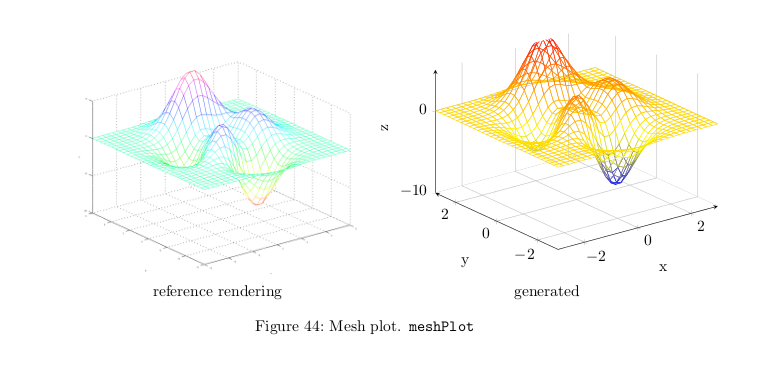
\includegraphics[width=\textwidth]{figures/pgfplots-surface-cutoff.png}
\end{bug}

\begin{bug}[prio=1]
    内部 coordmath 框架：并未处处使用
\end{bug}

\begin{bug}[prio=1]
    \verb|log number format code| 是全局变量，无法为单个坐标轴设置。

    \verb|log ticks with fixed point| 也是如此。
\end{bug}

\begin{bug}
    若表格含空行，则无法在 pgfplots 坐标轴内手动加载它：
    scanline 回调处于激活状态
\end{bug}

\begin{bug}
    \verb|ybar legend| 不包含 \verb|ybar|（sourceforge 3482770）
\end{bug}

\begin{bug}
    \verb|refstyle| 只包含引用样式的部分信息。（sourceforge 3482770）
\end{bug}

\begin{bug}
    在 \verb|\legend| 内以方括号作为首字符会导致失败：
    \verb|\legend{[\ion{Ne}{2}],...}|。

    原因：\verb|\legend| 命令没有在每个条目前正确插入 \verb|[]|
    （本应如此）。
\end{bug}

\begin{bug}
    给 \verb|\addplot| 选项添加 \verb|error bars/.cd| 会导致
    \verb|\ref| 图片失败。

    问题显然在于键过滤：它丢弃了 \verb|/pgfplots/.cd|，却保留了
    \verb|error bars/.cd|。
\end{bug}

\begin{bug}[epic=quiver]
    quiver 图：裁剪路径不考虑箭头路径
\end{bug}

\begin{bug}
    对齐缺陷：axis x line=middle 与 yshift 组合会错误地移动 xlabel：
        \todosp{已注释的最小示例，因为 TeX 时会报错}
%%%%%\begin{minimal}
%%%%%\documentclass{report}
%%%%%\usepackage{pgfplots}
%%%%%\pgfplotsset{compat=1.3}
%%%%%
%%%%%\begin{document}
%%%%%  \begin{tikzpicture}
%%%%%      \draw (0,0) circle (5pt);
%%%%%    \begin{scope}[yshift=-3cm]
%%%%%    \begin{axis}[width=10cm,height=3cm,xlabel={$x$},
%%%%%        axis x line = middle]
%%%%%      \addplot coordinates {
%%%%%        (0,1) (1,-1) (2,1)
%%%%%      };
%%%%%    \end{axis}
%%%%%    \end{scope}
%%%%%  \end{tikzpicture}
%%%%%\end{document}
%%%%%\end{minimal}
    %
    在图中使用 \verb|xlabel style = {yshift=3cm}| 会正确定位 x 标签
    （回到其默认位置）。
\end{bug}

\begin{bug}
    由于嵌套的 scope，无法在 pgfplots 命令中使用裁剪路径。

    复现：尝试给某个图指定 \verb|\addplot+[/tikz/clip]|。
\end{bug}

\begin{bug}
    \verb|\pgfplotsforeachungrouped| 不能像 \verb|\foreach| 那样组合
    三个或更多参数

    （见 \url{https://tex.stackexchange.com/q/433059}。）
\end{bug}

\begin{bug}
    下面这个 latex 文件的示例在第二次运行 latex 时报以下错误。
    第一次运行正常。用 dvilualatex 和普通 latex 都如此，
    二者均来自 TexLive 2011。

    错误：
    %
\begin{verbatim}
...
(/usr/local/texlive/2011/texmf-dist/tex/generic/tex4ht/color.4ht)
(/usr/local/texlive/2011/texmf-dist/tex/generic/tex4ht/html4.4ht)
(/usr/local/texlive/2011/texmf-dist/tex/generic/tex4ht/html4-math.4ht))
(./epub.aux)
! Missing \endcsname inserted.
<to be read again>
                   \protect
l.30 \ref{govconsumptionlegend}

?
\end{verbatim}

\begin{verbatim}
\makeatletter

\def\HCode{\futurelet\HCode\HChar}\def\HChar{\ifx"\HCode\def\HCode"##1"{\Link##1}\expandafter\HCode\else\expandafter\Link\fi}\def\Link#1.a.b.c.{\g@addto@macro\@documentclasshook{\RequirePackage[#1,html]{tex4ht}}\let\HCode\documentstyle\def\documentstyle{\let\documentstyle\HCode\expandafter\def\csname tex4ht\endcsname{#1,html}\def\HCode####1{\documentstyle[tex4ht,}\@ifnextchar[{\HCode}{\documentstyle[tex4ht]}}}

\makeatother

\HCode "xhtml,png,charset=utf-8".a.b.c.


\documentclass[11pt,a4paper]{book}

\def\pgfsysdriver{pgfsys-tex4ht.def}
\usepackage{pgfplots}

\pgfplotsset{width=\textwidth,compat=1.3,every axis/.append style={font=\footnotesize},cycle list name=black white}

\begin{document}
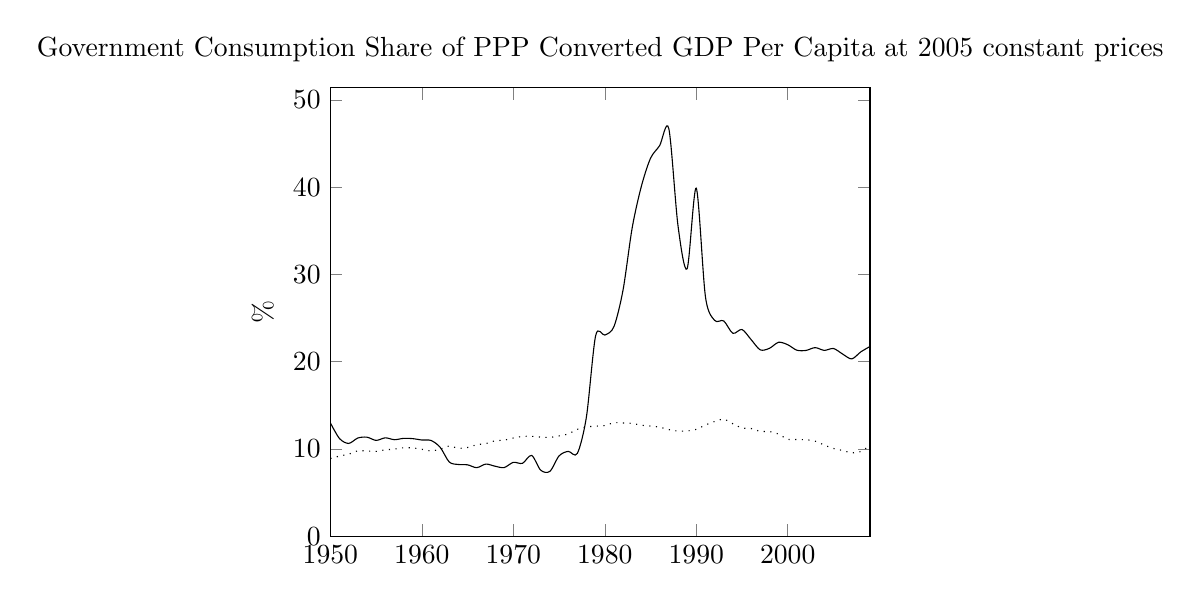
\begin{tikzpicture}

\begin{axis}[ylabel=\%,x tick label style={ /pgf/number format/1000 sep=},ymin=0,xmin=1950,xmax=2009,legend to name=govconsumptionlegend,title=Government Consumption Share of PPP Converted GDP Per Capita at 2005 constant prices]
\addplot[smooth,solid] coordinates {
(1950,12.98732304) (1951,11.18937899) (1952,10.63447043) (1953,11.25741618) (1954,11.35201741) (1955,10.98310036) (1956,11.27808626) (1957,11.06275337) (1958,11.21626046) (1959,11.18458192) (1960,11.02716074) (1961,10.97486816) (1962,10.19712891) (1963,8.50170024) (1964,8.220444391) (1965,8.181873469) (1966,7.859215042) (1967,8.269806768) (1968,8.023789126) (1969,7.867343418) (1970,8.469691612) (1971,8.352726749) (1972,9.263915297) (1973,7.560088984) (1974,7.436700475) (1975,9.207375031) (1976,9.725811776) (1977,9.495010597) (1978,13.74144043) (1979,22.99348928) (1980,23.05639171) (1981,24.02424559) (1982,28.25010594) (1983,35.38307779) (1984,40.11885923) (1985,43.3304334) (1986,44.7847218) (1987,46.7237337) (1988,35.62924609) (1989,30.65659214) (1990,39.89428582) (1991,27.48910619) (1992,24.75024034) (1993,24.68286164) (1994,23.26013887) (1995,23.69594547) (1996,22.53334681) (1997,21.35901868) (1998,21.53873871) (1999,22.22968487) (2000,21.95238646) (2001,21.3231532) (2002,21.29835897) (2003,21.6183452) (2004,21.30177929) (2005,21.51748623) (2006,20.88675316) (2007,20.32549306) (2008,21.13794484) (2009,21.75075984)
};
\addlegendentry{Country 1}
\addplot[smooth,dotted] coordinates {
(1950,8.90574995) (1951,9.181850378) (1952,9.4040808) (1953,9.790597533) (1954,9.766571438) (1955,9.721345475) (1956,9.898347958) (1957,9.986947451) (1958,10.13725015) (1959,10.11995062) (1960,9.9669931) (1961,9.781482565) (1962,9.968596797) (1963,10.33417822) (1964,10.07453069) (1965,10.17668623) (1966,10.4859246) (1967,10.6188237) (1968,10.93369976) (1969,11.01396095) (1970,11.25808879) (1971,11.43128231) (1972,11.45138898) (1973,11.36045323) (1974,11.33276575) (1975,11.50069671) (1976,11.72466305) (1977,12.25394557) (1978,12.52158998) (1979,12.61603185) (1980,12.68712893) (1981,13.01282874) (1982,12.97669774) (1983,12.92432378) (1984,12.72145426) (1985,12.63447969) (1986,12.49591698) (1987,12.22704263) (1988,12.05291461) (1989,12.07675903) (1990,12.25254614) (1991,12.74485006) (1992,13.14305947) (1993,13.41082617) (1994,12.89670369) (1995,12.41585298) (1996,12.34588672) (1997,12.01926401) (1998,12.00221677) (1999,11.69852271) (2000,11.11468531) (2001,11.08248726) (2002,11.05693806) (2003,10.89817902) (2004,10.44900187) (2005,10.05582475) (2006,9.829361577) (2007,9.567882534) (2008,9.714898563) (2009,10.42225882)
};
\addlegendentry{Country 2}
\end{axis}\end{tikzpicture}

\ref{govconsumptionlegend}

\end{document}
\end{verbatim}
\end{bug}

\begin{bug}[prio=2]
    \#3213889 hyperref 框对竖直标签位置错误
    问题描述与可能的修复见
    \url{http://tex.stackexchange.com/questions/13364/how-to-make-pgfplots-vertical-labels-have-proper-hyperref-erence-box}
\end{bug}

\begin{bug}[prio=1]
    崩溃：
        \todosp{已注释的最小示例，因为 TeX 时会报错}
%%%%%\begin{minimal}
%%%%%\begin{tikzpicture}
%%%%%    \begin{axis}[
%%%%%        scale mode=scale uniformly,
%%%%%        x={(1pt,0pt)},
%%%%%        y={(-0.5pt,0.5pt)},
%%%%%        z={(0pt,1pt)},
%%%%%    ]
%%%%%
%%%%%    % addplot3 works (with 3d coords):
%%%%%    \addplot coordinates {
%%%%%        (0,0) (1,0) (0,1)
%%%%%    };
%%%%%
%%%%%    \end{axis}
%%%%%\end{tikzpicture}
%%%%%\end{minimal}
\end{bug}

\begin{bug}[prio=1]
    在 pgfplots 坐标系中使用 $0$ 并不一定意味着 ``无偏移''。这有误导性。
    缺陷 sourceforge \#3168030：
    %
        \todosp{已注释的最小示例，因为 TeX 时会报错}
%%%%%\begin{minimal}
%%%%%\documentclass[a4paper]{article}
%%%%%\usepackage{pgfplots}
%%%%%\begin{document}
%%%%%\begin{tikzpicture}
%%%%%    \begin{axis}[
%%%%%        enlarge x limits=false,
%%%%%        extra description/.code={
%%%%%            \draw[very thick] (axis cs:2.5,0) -- ++(rel axis cs:0,1.1)
%%%%%                node[above,align=center,font=\small]{important};
%%%%%        },
%%%%%    ]
%%%%%        \addplot coordinates{
%%%%%            (0,1)
%%%%%            (1,2)
%%%%%            (2,3)
%%%%%            (3,4)
%%%%%            (4,5)
%%%%%        };
%%%%%    \end{axis}
%%%%%\end{tikzpicture}
%%%%%
%%%%%\begin{tikzpicture}
%%%%%    \begin{axis}[
%%%%%        enlarge x limits=true,
%%%%%        extra description/.code={
%%%%%            \draw[very thick] (axis cs:2.5,0) -- ++(rel axis cs:0,1.1)
%%%%%                node[above,align=center,font=\small]{important};
%%%%%        },
%%%%%    ]
%%%%%        \addplot coordinates{
%%%%%            (0,1)
%%%%%            (1,2)
%%%%%            (2,3)
%%%%%            (3,4)
%%%%%            (4,5)
%%%%%        };
%%%%%    \end{axis}
%%%%%\end{tikzpicture}
%%%%%\end{document}
%%%%%\end{minimal}
\end{bug}

\begin{bug}[prio=1]
    图例的初始配置为 \verb|text depth=0.15em|，这对深度很大的图例条目
    （大分数或公式？）非常糟糕。
\end{bug}

\begin{bug}[-,prio=1]
    坐标轴线条组合样式无法为 3D 调整，因为它们求值得太早。
\end{bug}


\begin{bug}[-]
    groupplots + 额外花括号或 foreach 不兼容。
\end{bug}

\begin{bug}[-]
    numplotspertype 与 forget plot 以及 ybar interval 会产生错误。
\end{bug}

\begin{bug}[-]
    表达式绘图与空 'y' 会产生错误。或许显式地处理一下更好？
    （当某一输入行为空时在 hist 中出现）
\end{bug}

\begin{bug}[-]
    /pgfplots/samples at 与 /tikz/samples at 作用在同一坐标轴上。
    Tantau 说该键支持 foreach 语句，从而支持省略号记法。
    然而，当我想在 pgfplots 内使用两处或更多不同的省略号记法时，
    latex 崩溃！下面的示例说明了此问题：
    \verb|\addplot+[mark=none,variable={\t}, samples at = {\foreach \x in {0,10,...,180,200,...,340} {\x, }360}] ({sin(t*2)}, {cos(t)});|
    %
\begin{verbatim}
\documentclass[border=5pt]{standalone}
\usepackage{pgfplots}
\begin{document}
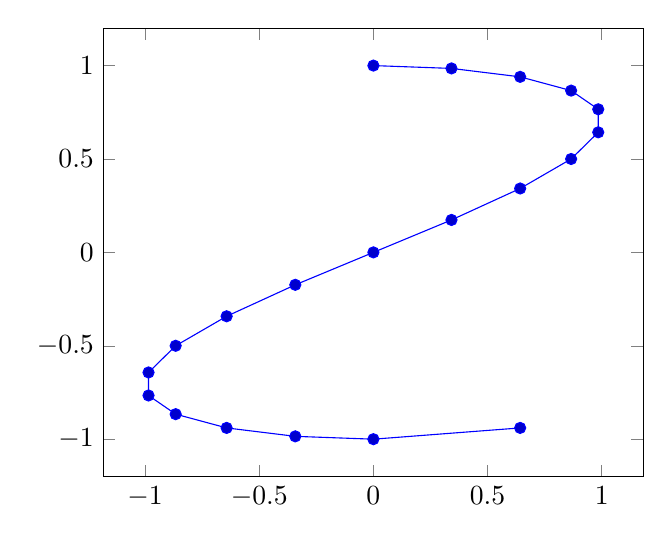
\begin{tikzpicture}
\begin{axis}
    \addplot+ [
        samples at={
%            0,10,...,360                % <-- works
            0,10,...,180,200,...,360    % <-- only evaluates up to ``180''
%            % both following lines cause an error
%            % (what could be an advantage of using `\foreach' instead of
%            %  directly using the above syntax?)
%            \foreach \x in {0,20,...,340} {\x, }360
%            \foreach \x in {0,10,...,180,200,...,340} {\x, }360
        },
    ] ( {sin(x*2)}, {cos(x)} );
\end{axis}
\end{tikzpicture}
\end{document}
\end{verbatim}
\end{bug}

\begin{bug}[-,prio=2,epic=clickable,epic=external]
    潜在不兼容：clickable 与 external。clickable 库写入 pgfplots.djs，
    可能引发多线程问题。
\end{bug}

\begin{bug}[-,epic=groupplots]
    groupplots：在一个 groupplot 中混用 2D/3D 不会重置 'zmin,zmax'？
\end{bug}

\begin{bug}[-]
    3D 坐标轴：很难与 tikz 取得 1:1 的对应。
\end{bug}

\begin{bug}[-]
    3D 坐标轴：提供对手动坐标轴配置的支持，
    - depth（n 向量），
    - 前景/背景，
    - 刻度标签坐标轴，
    - ……
\end{bug}

\begin{bug}[-]
    plot graphics：\verb|\ref| 图例不能正常工作
    \todosp{这里能否说得更具体些？}
\end{bug}

\begin{bug}[-,epic=ternary]
    ternary 坐标轴：'marker clipping' 不起作用（自然如此）
\end{bug}

\begin{bug}[-]
    contour：
    table/meta=2 的默认值是错的。
\end{bug}

\begin{bug}[-,prio=2]
    正常：'every node near coord/.append style={scale=0.7}'
    不正常：'every node near coord/.append style={scale=0.7},ybar'
    -$\leadsto$ 偏移与缩放的顺序很关键……
\end{bug}

\begin{bug}[-]
    dimension too large 健全性检查：TeX 改用最大值。
    或许可以检查一下？
\end{bug}

\begin{bug}[-,prio=2]
    view={0}{90} 且 enlargelimits=auto 并不总是令人满意：它禁用放大的限度，
    但对 contour 而言我希望保留。该怎么办？
\end{bug}

\begin{bug}[-,prio=1]
    有很多 .code 2 args 样式不支持其参数之间的空格。修复它。
\end{bug}

\begin{bug}[-,prio=2]
    contour external 尚不能处理显式提供的矩阵数据（mesh/rows 与 mesh/cols）。
\end{bug}

\begin{bug}[-,prio=2]
    contour external 不能正确处理 ordering 标志。
\end{bug}

\begin{bug}[-,epic=quiver]
    quiver/scale arrows 这个东西或许需要一个 "auto" 选项。若现在不加，
    以后大概永远也不会支持。
\end{bug}

\begin{bug}[-]
    对数图中的 `1.23456e4;' 会产生难以阅读的错误信息。
    改进此处的健全性检查。
\end{bug}

\begin{bug}[-,prio=2]
    'footnotesize' 的 title 样式不符合我的期望：它不考虑基线以下的深度。
    或者它是否需要一个 \verb|\strut|？
\end{bug}

\begin{bug}[-,epic=Usability]
    避免因数据范围限制而导致的 dimension too large 错误。
    示例：
    数据范围 = 0:6000
    视图范围 = 0:1
    $\leadsto$ 导致错误。
    但这很容易检测！只需以浮点数计算点坐标（在缩放完成之后）。然后在某处装一个
    过滤器。或许在 pointxyz 命令里装一个 ``事后'' 过滤器？

    重复项：
    若 pgfplots 简单地把结果裁剪到 TeX 的范围内，那个讨厌的 dimension too large
    消息大概就能避免。
\end{bug}

\begin{bug}[-]
    \verb|yticklabels={<list>}, extra y ticks={...}| 不兼容，因为 extra ticks
    共用同一套刻度排版例程（而该例程又会查询 <list>）。
    \todosp{这里能否也给一个能展示该缺陷的示例？}
\end{bug}

\begin{bug}[-]
    图例条目中的 'text depth' 与 'text width' 不兼容。
    问题：text width 是用 \verb|\begin{minipage}[t]| 实现的，故其内容全在深度内。
    设置 text depths 会覆盖高度！
\end{bug}

\begin{bug}[-,prio=1]
    '/pgfplots/table/.search also' 在 \verb|\addplot table| 期间被
    /.search also={/pgfplots} 覆盖。这不太好。
\end{bug}

\begin{bug}[-]
    无法给 addplot 提供 'disable log filter'（但它可能有用）
\end{bug}

\begin{bug}[-]
    FPU：atan 不检查无界输入。
\end{bug}

\begin{bug}[-]
    无界输入：改进警告信息：不应包含底层 FPU 参数。
\end{bug}

\begin{bug}[-]
    为单个坐标轴设置 'tickwidth=0' 的用户界面不太好：
    似乎需要 'xtick style={/pgfplots/tickwidth=0}' 才能做到……
    $\leadsto$ 我猜若 tickwidth 有 family 就能解决。类似 'draw'，
    且不会被 pgfplots 拉取。但那样键路径又成了问题。
\end{bug}

\begin{bug}[-]
    我见过对超大文件使用 'plot table' 会产生 pool size 问题
    —— 即便坐标全被过滤掉。
    换言之：代码不能简单地读取文件然后丢弃其内容。问题似乎在于使用
    table/x expr 等做的某种数学解析。'pool size = 控制序列名与文件名'
    $\leadsto$ 数学解析器可用 ifcsname 改进
\end{bug}

\begin{bug}[-]
    给坐标轴提供 zmin/xmax 会激活 3D 模式，这没问题 —— 但低维输入例程
    似乎失败。
\end{bug}

\begin{bug}[-]
    无法把 'scale' 作为参数提供给（3D）坐标轴
\end{bug}

\begin{bug}[-]
    对数坐标轴仍可能只得到*一个*刻度标签（我这里是 \verb|10^{-0.2}|）。
    这绝不应发生。范围约为 ymin=4.7e-1，ymax=9.5e-1
\end{bug}

\begin{bug}[-]
    3D 图绘图表达式中的 log samples
\end{bug}

\begin{bug}[-,epic=gnuplot]
    不同的对数底数与 gnuplot
\end{bug}

\begin{bug}[-]
    我尝试在一个坐标轴内放置一个命名坐标，再在另一个坐标轴中使用它。
    失败了。

    CF：坐标轴绘制在它自己的 picture 内，只有在全部绘制完后才会被平移。
    我猜这就是问题的根源。

    奇迹般地，我可以在 axis 环境之外使用该坐标。于是我得到了如下方案：
\end{bug}

\begin{bug}[-]
    plot coordinates 检查得不太好：
    1. 使用 addplot3 却只给两个坐标
    2. 给定 addplot 却提供三个坐标
       （绘图表达式也是如此）
\end{bug}

\begin{bug}[-]
    compat 相关的东西尚不完整：我想检查它何时真的必要
    （例如使用 'x dir' 时）
\end{bug}

\begin{bug}[-,epic=nodes near coords]
    nodes near coords 特性与标记一起使用时会产生意料之外的结果
    $\leadsto$ 这是由散点图的默认配置所致。
\end{bug}

\begin{bug}[-]
    ybar 样式不会在 \verb|\label{}| 内被设置
\end{bug}

\begin{bug}[-]
    semilog 图的 axis equal 不正确（？）
\end{bug}

\begin{bug}[-]
    向后兼容问题：
    坐标轴说明再也不能包含 /pgfplots/ 样式了！这是键路径问题 :-(
\end{bug}

\begin{bug}[-]
    缺陷：在空坐标轴中，'\verb|xtick=\empty|' 被忽略。
\end{bug}

\begin{bug}[-]
    自动刻度标注有时会产生不一致或令人困惑的标签：
    1. engineering 与 fixed 数字样式被混淆。
    2. 若某坐标轴范围小到标签只在第三位小数上不同，仍只使用两位小数。
\end{bug}

\begin{bug}[-]
    3D：误差棒与堆叠图需要更新。

    这还有效吗？前段时间做过一次大改……
\end{bug}

\begin{bug}[-,prio=2]
    interp 着色器在 evince 中显示为透明。

    （肯定是 evince 的缺陷。）该怎么办？
\end{bug}

\begin{bug}[-]
    addplot3 与 addplot：
    %
\begin{verbatim}
  3D:  the use of \addplot3 and \addplot is not sanitized properly
    Possibilities:
    -  used \addplot  when \addplot3 should have been used
    -  used \addplot3 where \addplot should have been used.
     What can happen here!? Shouldn't this work in every case?

- The "xtick" value is not applied unless there is a coordinate in the x range:
    $\leadsto$ that's the handling of empty figures...
    not working:
      \begin{axis}[xtick=0]
      \end{axis}
    not working:
      \begin{axis}[xmin=-5,xmax=5,xtick=0]
      \end{axis}
    not working:
      \begin{axis}[xmin=-5,xmax=5,xtick=0]
        \addplot coordinates { (-10, 0) };
      \end{axis}
    working:
      \begin{axis}[xmin=-5,xmax=5,xtick=0]
        \addplot coordinates { (0, 0) };
      \end{axis}
\end{verbatim}
\end{bug}

\begin{bug}[-,prio=1]
    在 3D 情形，axis [xyz] line != box 时，只有一个超平面。
    我的实现只在要么全为 box、要么全为 'middle' 时才工作。
\end{bug}

\begin{bug}[-,prio=3]
    3D 情形：刻度/网格线位于坐标轴线条之上。这导致质量不佳。

    ……但迄今为止还没人抱怨过
\end{bug}

\begin{bug}[-,prio=1]
    若整幅图被旋转（sidewaysfigure），javascript 相关内容不起作用。
\end{bug}

\begin{bug}[-,prio=1]
    javascript：与 external 库不兼容：
    1. 文件名：\verb|\jobname| 含 catcode 不兼容的字符，而那个古怪的
       insdljs 宏包试图用这些字符组装宏。
       $\leadsto$ 已修复；我直接用 pgfplotsJS 作为临时文件名。
    2. 图片本身的形式被破坏
       $\leadsto$ 若在加载 pgf 之前使用
       \verb|\usepackage{eforms}| 即可修复。
       原因：\verb|\begin{Form}| 与 pgf externalization 的 shipout 花招
       互相冲突。\verb|\begin{Form}| 必须在 pgf 的 shipout 花招之前。
    3. \verb|\includegraphics |不保留 PDF 表单。
\end{bug}

% -----------------------------------------------------------------------------

\begin{bug}[closed,epic=polar]
    极坐标轴：
    %
    \begin{itemize}
        \item \ok 有误，因为 'near ticklabel' 锚点使用 pointunitx，
            而它未为极坐标轴正确初始化。
        \item  axis equal（不 100% 确定，但已关闭。若重现会另开新工单）
        \item \ok 需为 X 轴禁用数据缩放。
        \item \ok 自动刻度标签仅在 disabledatascaling 的情形下工作
    \end{itemize}
\end{bug}

\begin{bug}[closed]
    external 库 + dvi/ps + windows：似乎 ';' 不起作用；用 '\&' 分隔命令
\end{bug}

\begin{bug}[closed]
    view normal vector 不能正确考虑 plot box ratio 与 x dir
\end{bug}

\begin{bug}[closed]
    clickable 与 Windows Acrobat Reader 9 据报告存在失败

    这仍然有效吗？
\end{bug}

\begin{bug}[closed]
    pdfpages（最新版）、MiKTeX 与 tikz external 库不兼容
    （与 shipout 例程有关）
\end{bug}

\begin{bug}[closed]
    mesh/patch 图：
    - jump 与 z buffer=sort 大概不能协同工作
\end{bug}

\begin{bug}[closed]
    在文档末尾给出提示："Package pgfplots: 考虑使用导言区命令
    \verb|\pgfplotsset{compat=1.3} 以改进标签 placement|"
\end{bug}

\begin{bug}[closed]
    contour external 应允许对 scanline 结束标记有不同处理方式。
    gnuplot 需要空行；据我所知 matlab 不处理它们。
\end{bug}

\begin{bug}[closed]
    '\verb|\\|' 列表格式的自动检测有缺陷：它应当且仅当最后一个元素是
    '\verb|\\|' 时返回真，而不是只要 '\verb|\\|' 出现在参数内就返回真。
\end{bug}

\begin{bug}[closed]
    '\verb|\addplot[only marks]|' 不指定图标记；需要显式写 'mark=*'。
    这令人困惑……

    另见
    \url{https://sourceforge.net/tracker/?func=detail&atid=1060656&aid=3045389&group_id=224188}
\end{bug}

\begin{bug}[closed]
    axis lines 与 3D：某些刻度线不绘制，见手册示例
\end{bug}

\begin{bug}[closed]
    检查 compat=newest 下刻度缩放标签的放置。
    $\leadsto$ 我已为 2d 与 3d 改进了它们。
    $\leadsto$ 我想还需要一些进一步检查。
\end{bug}

\begin{bug}[closed]
    考虑为坐标轴线提供基础级命令——这也应允许 \verb|\pgfpathclose|！
\end{bug}

\begin{bug}[closed]
    当两条坐标轴线相交时，extra ticks 会被坐标轴线的刻度特例禁用。
\end{bug}

\begin{bug}[closed]
    刻度线的裁剪未考虑坐标轴线的线宽。
    \url{http://tex.stackexchange.com/questions/91517/how-to-make-the-tick-thickness-as-the-axis-line/91645#91645}
\end{bug}

\begin{bug}[closed]
    回归：pgf 图片 externalization 损坏，见评论
    \url{https://sourceforge.net/p/pgf/bugs/229/}
\end{bug}

\begin{bug}[epic=layers,closed]
    \url{http://tex.stackexchange.com/questions/104010/why-does-loading-pgfplots-after-tikz-break-the-default-layers-in-a-tikzpicture}
    仍然有效。

    解决方案：backgrounds 库必须在 pgfplots 之后加载。显然，backwards 图层相关
    内容覆盖了 backgrounds 库的钩子。
\end{bug}

\begin{bug}[prio=2,closed]
    关于对数坐标轴中 extra ticks 的某问题已在
    \url{http://tex.stackexchange.com/questions/148703/bug-pgfplots-extra-ticks} 报告。
\end{bug}

\begin{bug}[closed]
    在 3D 坐标轴中，\verb|(axis cs:0,0)| 与 \verb|(axis cs:0,0,0)| 不等价！
    与 datascale 变换有关的什么东西破坏了它。
    \url{http://tex.stackexchange.com/questions/223623/pgfplots-tikz-interoperability-and-axis-equal}
\end{bug}

\begin{bug}[closed]
    把两个带 \verb|fill between| 指令的坐标轴写进同一个 \verb|tikzpicture| 会失败，
    因为第一个坐标轴中的 \verb|fill between| 在目标图层上安装了一个裁剪路径
    —— 于是第二个 \verb|fill between| 就被直接裁掉了。

    见 \url{http://tex.stackexchange.com/questions/207450/fillbetween-from-pgfplots-does-not-work-inside-groupplots/286771?noredirect=1#comment695143_286771}
    及其重复工单。

    见 \verb|pgfplotsfillbetween@ensure@clipping@on@layer|
\end{bug}

\begin{bug}[closed]
    closedcycle 在 3D 坐标轴中似乎失败：
    \url{http://tex.stackexchange.com/questions/285144/how-to-plot-multiple-2d-filled-graphs-in-3d-with-tikz}
\end{bug}

\begin{bug}[closed]
    external 库：若开启 force remake，则不生成 MD5
\end{bug}

\begin{bug}[closed]
    在某坐标轴的选项内本地定义 colormap 不会把结果传到 colorbar
\end{bug}

\begin{bug}[closed]
    坐标映射错误：第一个图不从 $x=0$ 开始！
    %
\begin{verbatim}
  \begin{tikzpicture}
%  \tracingmacros=2 \tracingcommands=2
    \begin{axis}[
      %xbar stacked,
      stack plots=x,/tikz/xbar,
      area legend,
        xmajorgrids,
      %disabledatascaling,
      legend pos=outer north east,
      enlarge y limits=0.3,
      extra description/.code={%
      \pgfpathcircle{\pgfplotspointaxisorigin}{5pt}%
      \pgfusepath{fill}%
      },
      ]
      \addplot table [x index=1,y expr=\coordindex] {\mytable};
      \addplot+[yshift=5pt]table [x index=2,y expr=\coordindex] {\mytable};
      \addplot+[yshift=10pt] table [x index=3,y expr=\coordindex] {\mytable};
      \addplot+[yshift=15pt] table [x index=4,y expr=\coordindex] {\mytable};
    %  \fill (0,0) circle (3pt);
      \legend{Cat1,Cat2,Cat3,Cat4}
    \end{axis}
  \end{tikzpicture}
\end{verbatim}
\end{bug}

\begin{bug}[closed]
    缺陷：fill between 与 error bars 不兼容
    \url{http://tex.stackexchange.com/questions/281379/pgfplots-issues-with-fillbetween}
\end{bug}

\begin{bug}[closed]
    dateplot 库：若不使用 date ZERO，精度问题会导致意外的舍入效应。

    或许我得以编程方式计算 dateZERO？

    \url{https://sourceforge.net/p/pgfplots/bugs/96/}
\end{bug}

\begin{bug}[closed]
    特性 \verb|/pgfplots/compat/BB/1.8|
    （\verb|clip bounding box=upper bound|）在下图中产生问题：
    %
\begin{verbatim}
\documentclass{article}
\usepackage{pgfplots}
    \usetikzlibrary{pgfplots.fillbetween}
    \pgfplotsset{
%        compat=1.7,     % works as expected
        compat=1.8,     % enlarges bounding box
        %/pgfplots/compat/BB/1.7,
    }
\begin{document}
\begin{tikzpicture}
    \begin{semilogyaxis}
        \addplot [name path=up]
            table [x=time,y=energy] {
                time    energy
                1861.31    5.16e11
                2099.71    7.23e13
            };
        \addplot [name path=down]
            table [x=time,y=energy] {
                time    energy
                1875.5    2.53e11
                2099.75    2.87e13
            };
        \addplot [black!20]
            fill between [of=up and down];  % commenting this also works
    \end{semilogyaxis}
\end{tikzpicture}
\end{document}
\end{verbatim}
    %
    下面这个也坏了，可用 \verb|compat/BB/pre 1.3| 修复：
    %
\begin{verbatim}
\documentclass{standalone}
\usepackage{pgfplots}
    \pgfplotsset{compat=1.13}
\begin{document}
        \pgfplotsset{
            xmin=-1,
            xmax=1,
            ymin=-1,
            ymax=1,
            legend entries={x},
            legend pos=outer north east,
            xlabel=$x$,
            ylabel=$y$,
            %/pgfplots/compat/BB/pre 1.3,
        }%
    \begin{tikzpicture}[baseline]
        \draw[-stealth,red] (-1,-1) -- (0,0);

        \begin{axis}[
            cell picture=false,
        ]
            \addplot coordinates {(-5,-5) (5,5)};
        \end{axis}
    \end{tikzpicture}
\end{document}
\end{verbatim}
\end{bug}

\begin{bug}[closed]
    lua 后端：以下代码产生不同结果：
    %
\begin{verbatim}
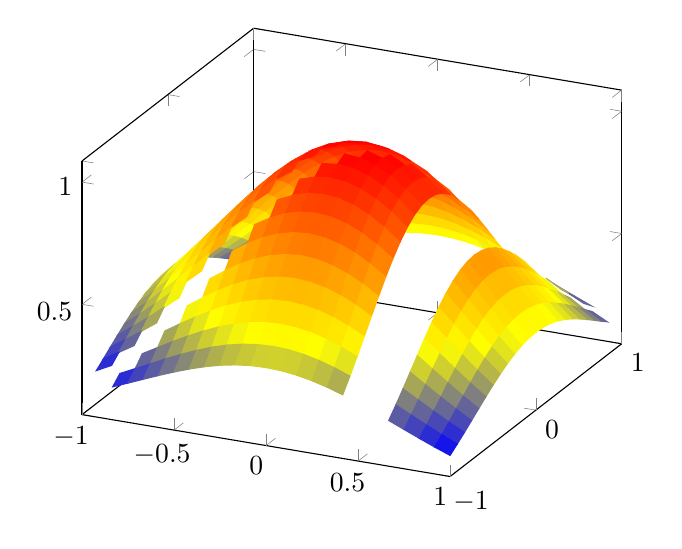
\begin{tikzpicture}
    \begin{axis}[shader=flat corner,domain=-1:1]
        \addplot3[surf,point meta={abs(x-y)<0.1 || abs(x-0.5)<0.1 ? nan : z}]
            {exp(-x^2-y^2)};
    \end{axis}
\end{tikzpicture}
\end{verbatim}
\end{bug}

\begin{bug}[closed]
    带空行的间断图与 lua 后端不能协同工作！

    见手册 ``interrupted plots'' 一节的第一个示例！
\end{bug}

\begin{bug}[closed]
    3.0.1 带了一个错误的修复！它完全错了……

    已在 pgf 3.0.1 中修复（撰写本文时尚未发布）

    数学缺陷：

    floor 似乎坏了？这还有效吗？见
    \url{http://tex.stackexchange.com/questions/118406/how-to-graph-floor-ceiling-functions-in-latex-pgfplots}

    int 似乎坏了：
    \url{http://tex.stackexchange.com/questions/249316/runaway-argument-using-int-function-in-pgfplots}
\end{bug}

\begin{bug}[closed]
    lua 后端若与 surf 图中的 jumps 一起使用会产生乱码：
    %
\begin{verbatim}
\documentclass{standalone}
\usepackage{pgfplots}
\usepgfplotslibrary{patchplots}
    \pgfplotsset{compat = 1.12}
    \pgfkeys{/pgf/declare function={param=2.0;}}
\begin{document}
    \begin{tikzpicture}
        \begin{axis}[view={40}{50}]
            \addplot3 [
                surf, domain = 0:1, y domain = 0:1, unbounded coords=jump,
                shader=interp, samples = 25]
            {x^(-param-1)*y^(-param-1)*(x^(-param)+y^(-param)-1)^(-1/param-2)+param*x^(-param-1)*y^(-param-1)*(x^(-param)+y^(-param)-1)^(-1/param-2)};
        \end{axis}
    \end{tikzpicture}
\end{document}
\end{verbatim}
\end{bug}

\begin{bug}[prio=9,closed]
    lualatex 缺陷：带 \verb|y=\coordindex| 的表格不能工作
    \url{http://tex.stackexchange.com/questions/227700/xbar-plots-in-pgfplots-1-12-gives-empty-y-axis-range-warning/227856#227856}
\end{bug}

\begin{bug}[closed]
    让 LUA 兼容 LUA 5.3

    数学库中下列函数已弃用：atan2、cosh、sinh、tanh、pow、frexp、ldexp。
    可用 x^y 替换 math.pow(x,y)；可用 math.atan 替换 math.atan2，它现在接受
    一个或两个参数；可用 x * 2.0^exp 替换 math.ldexp(x,exp)。其余运算可使用
    外部库，或在 Lua 中自行实现。
\end{bug}

\begin{bug}[closed]
    回归：pgf 2.10 的 atan 兼容性损坏：
    %
\begin{verbatim}
\documentclass{article}
\usepackage{pgfplots}
    \pgfplotsset{compat=1.9}
\begin{document}
\begin{tikzpicture}
    \begin{axis}[
    ]
        \addplot [mark=none,color=blue, samples=500] {rad(atan(x))};
    \end{axis}
\end{tikzpicture}
\end{document}
\end{verbatim}
    %
    无法编译
\end{bug}

\begin{bug}[closed]
    已采纳

    当 compat=1.11 激活时，数学函数 transformdirectionx 是错的
    （在以下上下文里），但该示例在 compat=1.10 下曾正常工作
\begin{verbatim}
\documentclass{standalone}
\usepackage{pgfplots}
    \pgfplotsset{compat=1.11}
\begin{document}
\begin{tikzpicture}
%\tracingcommands=2\tracingmacros=2
    \begin{axis}[xmin=0,xmax=5,ymin=0,ymax=5]
        \draw [ultra thin] (axis cs:0,0) grid [step={transformdirectionx(1)}] (axis cs:4,5);
    \end{axis}
\end{tikzpicture}
\end{document}
\end{verbatim}
    %
    此处建议的修复：\verb|step=1|。问题在于那个允许用 \verb|(0,0)| 代替
    \verb|(axis cs:0,0)| 的特性。

    理想情况下，旧代码应仍能工作（或给出报错）。
\end{bug}

\begin{bug}[closed]
    自 1.11 起，缩放图中弧的半径不正确。

    1.11 用 axis cs 替换了 pgfpointxy —— 但本例中它需要用 axis direction cs！

    建议方案：实现一个特殊的 arc，替换坐标系。

    \url{http://sourceforge.net/p/pgfplots/bugs/73/}
\end{bug}

\begin{bug}[prio=10,closed]
    由于 1.11 新的 ``replace pgfpoint'' 特性，pgfplots 中的 arc 坏了。

    见 \url{http://www.mrunix.de/forums/showthread.php?76557}
\end{bug}

\begin{bug}[closed]
    fillbetween 在 groupplots 内不能工作：
    \url{http://tex.stackexchange.com/questions/207450/fillbetween-from-pgfplots-does-not-work-inside-groupplots}

    与 cell picture 问题重复
    \url{http://tex.stackexchange.com/questions/227775/pgfplot-image-messed-up-with-newer-texlive}
\end{bug}

\begin{bug}[closed]
    set layers 与 colorbar 不能协同工作。实际上它只是
    \verb|cell picture=false|，位于 \verb|pgfplots@BEGIN@cell@picture@DISABLED| 某处。

    我试用了一个补丁（见 \verb|~/tmp/cellpicturefalse.diff|）
    %
\begin{verbatim}
\documentclass{standalone}
\usepackage{pgfplots}
    \pgfplotsset{width=7cm,compat=1.11}
\begin{document}
    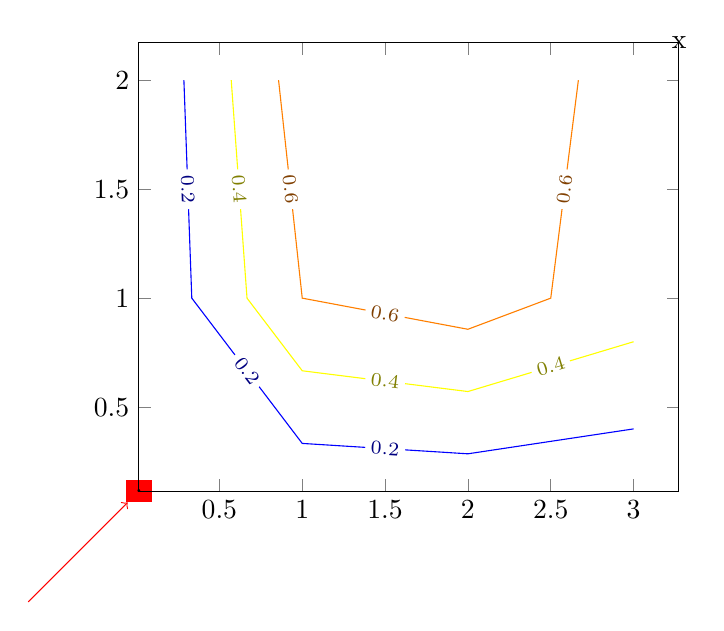
\begin{tikzpicture}
        \node[fill=red] (XYZ) at (40pt,40pt) {.};
        \draw[red,->](0cm,0cm) -- (XYZ);

        \pgfplotsset{cell picture=false}
        %\tracingmacros=2 \tracingcommands=2
        \begin{axis}[
            clip=false,
            name=axisA,
            at={(XYZ)},
        ]
        \addplot[contour prepared]
            table {
                2 2 0.8
                0.857143 2 0.6
                1 1 0.6
                2 0.857143 0.6
                2.5 1 0.6
                2.66667 2 0.6
                0.571429 2 0.4
                0.666667 1 0.4
                1 0.666667 0.4
                2 0.571429 0.4
                3 0.8 0.4
                0.285714 2 0.2
                0.333333 1 0.2
                1 0.333333 0.2
                2 0.285714 0.2
                3 0.4 0.2
            };
        \end{axis}

        %\begin{axis}[at={(axisA.north east)},anchor=north west]
        %\addplot {x};
        %\end{axis}
        \node at (current axis.right of north east) {x};
    \end{tikzpicture}
\end{document}
\end{verbatim}
    %
    该问题的另一表现：

    注意：这可用 \verb|/pgfplots/compat/BB/pre 1.3| 解决！
    %
\begin{verbatim}
\documentclass{standalone}
\usepackage{pgfplots}
\begin{document}
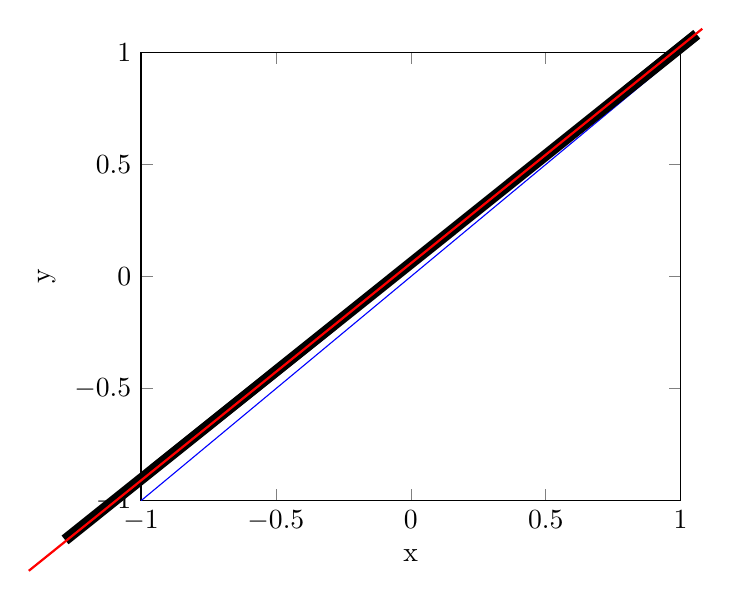
\begin{tikzpicture}
    \pgfplotsset{
        compat=1.11,
        samples=2,
        set layers, cell picture=false,
    }
\tracingmacros=2 \tracingcommands=2
\begin{axis}[
    xlabel=x,ylabel=y,
xmin=-1,
xmax=1,
ymin=-1, ymax=1,
]
\addplot coordinates {(-5,-5) (5,5)};
\end{axis}
\draw[line width=4pt] (-27.42155pt,-14.14372pt) -- (200.83115pt,168.5547pt);
    \draw[red,thick] (current bounding box.south west) -- (current bounding box.north east);
 % \message{FINAL (bad) size: (\the\pgf@picminx,\the\pgf@picminy) -- (\the\pgf@picmaxx,\the\pgf@picmaxy)^^J}%

\end{tikzpicture}
\end{document}
\end{document}
\end{verbatim}
    %
    此处的一些备注：
    %
    \begin{itemize}
        \item \verb|\draw[line width=4pt] (-27.42155pt,-14.14372pt) -- (200.83115pt,168.5547pt);|
            似乎是正确的 bb。
        \item 给 \verb|pgf@procotolsizes| 打补丁以输出
            \verb|\message{pgf@protocolsizes: (\the\pgf@picminx,\the\pgf@picminy) -- (\the\pgf@picmaxx,\the\pgf@picmaxy)^^J}%|
            显示存在一个巨大的 BB 条目 \verb|(584.9945pt,485.99854pt)|
        \item 它属于 \verb|clippath@install|，一旦准备好 description cs 即被使用。
            不过问题似乎出在 clippath 准备内部 —— 为何它要用这么大的值？
        \item description cs 在 \verb|\pgfplots@low@level@shape@INNER@define| 期间使用。
    \end{itemize}
\end{bug}

\begin{bug}[closed]
    luabackend：若数学表达式中大括号数目不平衡，则不产生错误信息
    %
\begin{verbatim}
    \addplot3[surf,domain=0:1,domain y=0:360,]
        {atan2(-sin(y),x-cos(y)}
\end{verbatim}
    %
    结果就是空的
\end{bug}

\begin{bug}[closed]
    已在 pgf cvs 中修复（pgfplots 未附带补丁）

    对超大曲面图，lua 后端受 save stack 问题困扰。

    我意识到 \verb|\pgfsetstrokecolor| 与 \verb|pgfsetcolor| 都对
    \verb|\color@pgfstrokecolor| 做全局赋值，这导致大量 retain 操作
    （因为 xcolor 在本地同样赋了同样的值）。

    去掉那个 \verb|\global| 对我的曲面图没影响 —— 只是 save stack 用得少多了。

    去掉它之后，$316\times 316 \approx 100000$ 节点的曲面图也能绘制。

    此外，代码审查显示没有理由让该赋值为全局。毕竟它与
    \verb|\pgfutil@colorlet{pgfstrokecolor}{..}| 组合，而后者是本地赋值的。

    注意：箭头尖端会带来差别！见此例：
    %
\begin{verbatim}
\documentclass{standalone}

\usepackage{tikz}

\begin{document}

\begin{tikzpicture}
    \useasboundingbox (-1,-1) (2,2);
%\tracingcommands=2\tracingmacros=2
    \begingroup
        {
        \pgfsetstrokecolor{green}
        }
        \pgfscope
        \draw[-stealth] (0,1) -- (1,1);
        \endpgfscope
    \endgroup

\end{tikzpicture}
\end{document}
\end{verbatim}
    %
    从代码判断，箭头尖端似乎就是当初把它做成全局的\emph{唯一}原因。
\end{bug}

\begin{bug}[closed]
    图片 externalization 与 \verb|\ref| 不能开箱即用。这也影响 pgfplots 的
    crossref 图片。

    思路：对 cross ref 图片禁用 externalization！
\end{bug}

\begin{bug}[prio=10, closed]
    在点定义中省略 ``axis cs'' 会占用更多内存 —— 为何！？

    问题在于新特性需要挂接到 TikZ 的点代码，特别是 \verb|\tikz@checkunit|。
    而它调用数学解析器来检测数学单位 —— 却把数学结果丢弃。新特性需要把它
    切换到 FPU，这导致更高的内存占用与 CPU 时间。

    它为何会增加内存！？

    已解决并修复：FPU 中的缺陷（不必要地使用了 \verb|globaldefs|）
    %
\begin{verbatim}
Die in Version 1.11 eingeführte Neuerung, dass sich Koordinaten innerhalb der
axis-Umgebung auch ohne Angabe von axis cs: auf das Koordinatensystem beziehen,
halte ich für eine gute Verbesserung, da sie den Code verkürzt (und die
bisherigen Standardkoordinaten kaum benutzbar waren).

Allerdings bin ich auf ein Speicherproblem gestoßen. Lässt man in der
beigefügten Datei "axis cs:" weg, erhält man zwar die gleiche Graphik, aber auf
meinem Rechner (kubuntu 12.04, pdflatex, pgf 3.0.0) werden dann

1238915 words of memory out of 3000000
statt
990083 words of memory out of 3000000

benötigt. Außerdem dauert das Compilieren länger.

Der Effekt tritt auch außerhalb von foreach-Schleifen auf. Bei meinen Messungen
kostete der Verzicht auf axis cs pro 2D-Punkt zwischen 380 und 400 words of
memory.
\end{verbatim}

\begin{verbatim}
%==============================================================================
%
%  tikz_axiscs.tex                                                     140815
%  Beispiel zur Wirkung von axis cs: in \foreach-Schleife
%
%==============================================================================
\documentclass[a4paper,11pt]{article}
%------------------------------------------------------------------------------
%  packages
%------------------------------------------------------------------------------
%
\usepackage[utf8]{inputenc}
\usepackage{amsfonts,amsmath,amssymb} % Mathematik-Pakete der AMS
\usepackage{latexsym}  % Mathematische Symbole
\usepackage{color}     % Farben
\usepackage{ngerman}   % Deutsche Trennungsregeln
\usepackage{graphicx}  % Graphik-Paket
%
\usepackage{tikz}
\usepackage{pgfplots}
\pgfplotsset{compat=1.11,
  /pgfplots/every axis/.style={
    axis x line=center, axis y line=center,
    font={\footnotesize},
    xlabel style={below}, ylabel style={left},
    xlabel=\hspace*{-1.0 ex}\raisebox{-1.5 ex}{$x$},
    ylabel=\hspace*{-2.5 ex}\raisebox{-2.5 ex}{$y$}
  },
 /pgfplots/every tick/.style={black}
}
%------------------------------------------------------------------------------
\begin{document}
%------------------------------------------------------------------------------
%

  \begin{center}
    %
    \begin{tikzpicture}
      %
      % DGL: x' = f(x,y) = 1; y' = g(x,y) = -y+x^3-4*x+2
      % (x,y) \in [0,2.75]x[-0.75,2]
      % Richtungsfeld auf (18x18)-Gitter
      %
      \begin{axis}[width=8.0cm, height=8.0cm, xmin=0, xmax=2.75,
        ymin=-0.75, ymax=2, xtick={0.5,1}, ytick=\empty,
        xticklabels={$x_1$,$x_2$}]
        %
        % Richtungsfeld; Der Faktor in \delta steuert die Strichlänge
        \foreach \y in {-0.7,-0.55,...,1.85} {
          \foreach \x [evaluate=\x as \dxx using 1]
                      [evaluate=\x as \dyy using -\y+(\x)^3-4*\x+2]
                      [evaluate=\x as \delta using 17*sqrt((\dxx)^2+(\dyy)^2)]
                      [evaluate=\x as \dx using \dxx / \delta]
                      [evaluate=\x as \dy using \dyy / \delta]
                      [evaluate=\x as \s using \x-\dx]
                      [evaluate=\x as \t using \x+\dx]
                      [evaluate=\x as \u using \y-\dy]
                      [evaluate=\x as \v using \y+\dy]
          in {0,0.15,...,2.55} {
            \edef\temp{ % Makro \temp wegen axis-Befehl
              \noexpand \draw[gray] (axis cs:\s,\u) -- (axis cs:\t,\v); }
            \temp }
        } % \foreach \y
        % Lösung
        \addplot[very thick, samples=50, domain=0:2.5] { x*(x-1)*(x-2) };
        % Polygonzug
        \addplot[blue, very thick, mark=none] coordinates
                { (0,0) (0.5,1) (1,0.5625) };
        % Steigungsfähnchen in P1 und P2
        \draw[very thick] (0.45,1.044) -- (0.55,0.956);
        \draw[very thick] (0.95,0.641) -- (1.05,0.484);
        \filldraw[blue] (0.5,1)    circle (1.5pt);
        \filldraw[blue] (1,0.5625) circle (1.5pt);
        \node[blue, above] at (0.5,1.05)   { $P_1$ };
        \node[blue, above] at (1.1,0.5625) { $P_2$ };
        %
      \end{axis}
      %
    \end{tikzpicture}
    %
  \end{center}

%------------------------------------------------------------------------------
\end{document}
\end{verbatim}
\end{bug}

\begin{bug}[epic=boxplots, prio=6,closed]
    箱线图统计量的计算算法与其他工具不一致（会导致困惑）。此外，它甚至可能是
    错的。

    quartile quantile percentile（四分位、分位数、百分位）

    换一个更好的算法。

    \url{http://en.wikipedia.org/wiki/Quantile}

    \url{https://stat.ethz.ch/R-manual/R-patched/library/stats/html/quantile.html}

    \url{http://pbil.univ-lyon1.fr/Rweb/}

    \verb|quantile(x <- c(1,2, 3, 4,5), c(0.5), type = 5)|
\end{bug}

\begin{bug}[epic=boxplots,prio=6,closed]
    小样本量不能工作：试试 \verb|1,2,3|。这种情况下，箱线图处理程序的中位数与
    四分位数会取相同值，导致无法编译。
\end{bug}

\begin{bug}[epic=boxplots,closed]
    boxplots 在输入流中含有 NaN 时无法工作。
\end{bug}

\begin{bug}[epic=boxplots,closed]
    当坐标/重复坐标数目特殊时，box plots 似乎有一个 bug：
    \url{http://tex.stackexchange.com/questions/146663/pgfplots-fails-to-generate-boxplots-for-some-data-set?noredirect=1#comment332779_146663}
\end{bug}

\begin{bug}[closed]
    cart 到 polar 的坐标变换有精度问题；应改用 atan2

    见
    \url{http://tex.stackexchange.com/questions/195128/polar-plot-with-cartesian-values-lack-of-angular-precision-in-the-integrated-ar/195137#195137}
\end{bug}

\begin{bug}[+]
    histograms 与 density 选项似乎失效，对比
    \url{http://sourceforge.net/p/pgfplots/bugs/67/}

    以及一份（重复的？）报告
    %
\begin{verbatim}
\documentclass[tikz]{standalone}
\usepackage{pgfplots}
\begin{document}
\begin{tikzpicture}
    \begin{axis}
        \addplot+ [
            mark=none,
            fill=blue!10,
            hist={density},
        ] table [
            row sep=\\,
            y index=0,
        ] {
            data\\
            5.1 \\ 4.9 \\ 4.7 \\ 4.6 \\ 5.0 \\ 5.4 \\ 4.6 \\ 5.0 \\ 4.4 \\
            4.9 \\ 5.4 \\ 4.8 \\ 4.8 \\ 4.3 \\ 5.8 \\ 5.7 \\ 5.4 \\ 5.1 \\
            5.7 \\ 5.1 \\ 5.4 \\ 5.1 \\ 4.6 \\ 5.1 \\ 4.8 \\ 5.0 \\ 5.0 \\
            5.2 \\ 5.2 \\ 4.7 \\ 4.8 \\ 5.4 \\ 5.2 \\ 5.5 \\ 4.9 \\ 5.0 \\
            5.5 \\ 4.9 \\ 4.4 \\ 5.1 \\ 5.0 \\ 4.5 \\ 4.4 \\ 5.0 \\ 5.1 \\
            4.8 \\ 5.1 \\ 4.6 \\ 5.3 \\ 5.0 \\ 7.0 \\ 6.4 \\ 6.9 \\ 5.5 \\
            6.5 \\ 5.7 \\ 6.3 \\ 4.9 \\ 6.6 \\ 5.2 \\ 5.0 \\ 5.9 \\ 6.0 \\
            6.1 \\ 5.6 \\ 6.7 \\ 5.6 \\ 5.8 \\ 6.2 \\ 5.6 \\ 5.9 \\ 6.1 \\
            6.3 \\ 6.1 \\ 6.4 \\ 6.6 \\ 6.8 \\ 6.7 \\ 6.0 \\ 5.7 \\ 5.5 \\
            5.5 \\ 5.8 \\ 6.0 \\ 5.4 \\ 6.0 \\ 6.7 \\ 6.3 \\ 5.6 \\ 5.5 \\
            5.5 \\ 6.1 \\ 5.8 \\ 5.0 \\ 5.6 \\ 5.7 \\ 5.7 \\ 6.2 \\ 5.1 \\
            5.7 \\ 6.3 \\ 5.8 \\ 7.1 \\ 6.3 \\ 6.5 \\ 7.6 \\ 4.9 \\ 7.3 \\
            6.7 \\ 7.2 \\ 6.5 \\ 6.4 \\ 6.8 \\ 5.7 \\ 5.8 \\ 6.4 \\ 6.5 \\
            7.7 \\ 7.7 \\ 6.0 \\ 6.9 \\ 5.6 \\ 7.7 \\ 6.3 \\ 6.7 \\ 7.2 \\
            6.2 \\ 6.1 \\ 6.4 \\ 7.2 \\ 7.4 \\ 7.9 \\ 6.4 \\ 6.3 \\ 6.1 \\
            7.7 \\ 6.3 \\ 6.4 \\ 6.0 \\ 6.9 \\ 6.7 \\ 6.9 \\ 5.8 \\ 6.8 \\
            6.7 \\ 6.7 \\ 6.3 \\ 6.5 \\ 6.2 \\ 5.9 \\
        };
    \end{axis}
\end{tikzpicture}
\end{document}
\end{verbatim}
    %
    另见相关提交 \verb|1.8-12-g58161e9|

    来自 Jake：

    是的，density 图应当对面积归一化。它们本质上是概率密度函数的近似
    （这同样要求面积积分等于 1）。

    摘自维基百科关于直方图的条目：``直方图用于绘制数据的密度，也常用于密度
    估计：估计底层变量的概率密度函数。用于概率密度的直方图，其总面积总是归一化
    为 1。若 x 轴上各区间的长度都为 1，则直方图等同于相对频率图。''

    就当前实现而言，PGFPlots 中 density 直方图的代码似乎计算的是 bin 计数
    的相对频率，而非密度。它的用例应是计算概率质量函数，其中每个柱代表一个
    离散值（尽管对这一用途用 ycomb 图可能更正确）。
\end{bug}

\begin{bug}[+,prio=10]
    回归：stack plots 在下面这个示例中原本是可以工作的（至少到 1.8 为止），
    但现在失效了：
    %
\begin{verbatim}
\documentclass{standalone}
\usepackage{tikz}
\usepackage{pgfplots}
    \pgfplotsset{compat=newest}
    \pgfplotstableread{
        1   19.178  26.027  8.219   6.849   39.726 1
        2   54.795  21.918  4.110   6.849   12.329 1
        3   28.767  16.438  6.849   8.219   39.726 1
        4   63.014  2.740   2.740   2.740   28.767 2
        5   90.411  1.370   6.849   0.000   1.370  2
        6   15.068  2.740   16.438  8.219   57.534 2
        7   67.123  0.000   0.000   0.000   32.877 3
        8   72.603  6.849   5.479   0.000   15.068 3
        9   56.164  12.329  6.849   4.110   20.548 3
        10  50.685  4.110   8.219   1.370   35.616 3
    }\datatable
\begin{document}
\makeatletter
\begin{tikzpicture}
\begin{axis}[
    ybar stacked
]
    \addplot table[x index=0,y index=1] \datatable;
    \addplot table[x index=0,y index=2] \datatable;
    \addplot table[x index=0,y index=3] \datatable;
    \addplot table[x index=0,y index=4] \datatable;
    \addplot [stack plots=false] table[x index=0,y index=5] \datatable;
    \legend{Far,Near,Here,There,NotThere}
\end{axis}
\end{tikzpicture}
\end{document}
\end{verbatim}
\end{bug}

\begin{bug}[closed]
    当 set layers 生效时，fill between 装饰失效：
    %
\begin{minimal}
\documentclass{standalone}
\usepackage{pgfplots}
    \pgfplotsset{compat=1.10}
    \usepgfplotslibrary{fillbetween}
\begin{document}
\begin{tikzpicture}
    \begin{axis}[set layers]
        \addplot[
            domain=0:5,
            %postaction={decorate,red,thick},
            decorate,
            decoration={
                 soft clip,
                 soft clip path={domain=3:5},
             },
        ] {x^2};
    \end{axis}
\end{tikzpicture}
\end{document}
\end{minimal}
    %
    这段问题自 \verb|b7a8c0aad5a785e554d2e626c44123b0b17cf2cc| 起即存在，
    但该 bug 本身由来已久。

    我对比了 set layers 与 no layers 两种情况下装饰所用的输入路径 —— 它们不同。

    由 cell picture=false 引起！下面是一个精简示例：
    %
\begin{verbatim}
\begin{tikzpicture}
    \draw (0,0) circle (5pt);
    \begin{scope}[xshift=1cm]
    \path[name path=clipper] (1.5,-1) rectangle (4,2);
    \draw[
        postaction={decorate,draw,ultra thick},
        decoration={soft clip,soft clip path={
            (1.5,-1) rectangle (4,2)
            },
        },
    ]
        (0,0) -- (1,1) -- (2,1) -- (3,0);
    \end{scope}
\end{tikzpicture}%
\end{verbatim}
\end{bug}

\begin{bug}[closed]
    旧式 sampling 的避坑 bug：
    \verb|\pgfplotsforeachungrouped \x in {0,1,...,5000}| 在数值上不稳定
    （因为我不愿总是做昂贵的浮点比较……）

    \url{http://tex.stackexchange.com/questions/183369/tikz-and-pgfplot-problem-with-plotting}
\end{bug}

\begin{bug}[closed] % REJECT THIS. WON'T FIX
    \verb|shader=interp| 似乎用与 \verb|shader=faceted| 不同的方式生成三角形，
    对比
    %
\begin{verbatim}
\begin{tikzpicture}
    \begin{axis}
    \addplot3[surf,samples=2] {x*y};
    \end{axis}
\end{tikzpicture}

\begin{tikzpicture}
    \begin{axis}
    \addplot3[surf,samples=2,shader=interp] {x*y};
    \end{axis}
\end{tikzpicture}
\end{verbatim}
\end{bug}

\begin{bug}[closed]
    对 \verb|shader=interp| 使用 mesh 图例时，图例图像的包围盒不正确
    %
\begin{verbatim}
\begin{tikzpicture}
    \begin{axis}[legend entries=$xy$]
    \addplot3[surf,samples=2,shader=interp] {x*y};
    \end{axis}
\end{tikzpicture}
\end{verbatim}

\begin{minimal}
    \pdfcompresslevel=0
    \pdfminorversion=4
\documentclass{standalone}
\usepackage{pgfplots}
\begin{document}
\makeatletter
\fbox{%
    \tikzpicture
        \pgfplotsplothandlermesh@defaultlegend@img{%
            /pgfplots/shader=interp,
            % undo some shift hard-coded in the macro:
            %yshift=0.7cm,%
            %
            % this repairs it!
            %scale=1/0.4,
        }%
    \endtikzpicture
}%
\end{document}
\end{minimal}
\end{bug}

\begin{bug}[+]
    fillbetween 会配置 set layers —— 但这并未真正生效，见
    \url{http://tex.stackexchange.com/questions/170967/pgfplots-grid-lines-below-filling/171100#171100}
\end{bug}

\begin{bug}[+]
    3d centered 坐标轴：刻度线绘制不完整

    见
    %
\begin{minimal}
\documentclass[tikz,12pt]{standalone}
\usepackage{tikz,pgfplots,pgfplotstable}
    \pgfplotsset{compat=newest}
\begin{document}
\begin{tikzpicture}

%\pgfplotsset{every axis/.append style={tick style={line width=0.7pt}}}

\pgfplotstableread{
a b
-0.1 0.2
0.1 0.5
}\testdata

\begin{axis}[axis lines=center, ymin=-0.22,ymax=0.22,xmin=-0.1,xmax=.1  ]
    \addplot3 [color=blue,] table[x expr=0,y=a,z=b] {\testdata};
\end{axis}

\end{tikzpicture}
\end{document}
\end{minimal}
\end{bug}

\begin{bug}[closed]
    \verb|\addplot graphics| 内部即便是在 ConTeXt 上也尝试使用
    \verb|\includegraphics|

    这可以通过定义

    \verb|\def\includegraphicscompat[#1]#2{\externalfigure[#2][#1]}|

    并设置

    \verb|includegraphics cmd=\includegraphicscompat|

    来修复。这应由 PGF Plots 自动完成。
\end{bug}

\begin{bug}[closed]
    patchplots 库：对于非标准 patch 类型，图例编译失败

    给 \url{http://tex.stackexchange.com/questions/166570/color-and-legend-for-3d-surface}
    添加一个图例。
\end{bug}

\begin{bug}[closed]
    surf 图例在与插值着色一起使用时，包围盒是坏的

    给 \url{http://tex.stackexchange.com/questions/166570/color-and-legend-for-3d-surface}
    添加一个图例，并修复另一个相关 bug。
\end{bug}

\begin{bug}[closed]
    fill between：\verb|\addplot fill between [] ;| 中分号之前的路径命令
    被忽略/不被支持。
\end{bug}

\begin{bug}[closed]
    fill between：（实际上就是纯 tikz）在主路径之后添加 pins 会影响
    name path：
    %
\begin{minimal}
\documentclass{standalone}
\usepackage{tikz}
\usepackage{pgfplots}
    \usepgfplotslibrary{fillbetween}
\begin{document}
\begin{tikzpicture}
    \begin{axis}[smooth]

        % ... (der letzte) Pins jedoch schon
        % (beim Tauschen der 'pos'-Werte verursacht weiterhin der letzte das Problem)
        \addplot+[name path=A] table [x=x,y=y] {
x y z
0 2 3
0.5 -1 0
1 3 4
        }
        %    node [coordinate,pos=0.9, pin=above right:test] {}
            node [coordinate,pos=0.1, pin=above right:test] {}
        % folgt dem Pin noch ein Label, hat dieses keinen Einfluss
         %   node [pos=0.8] {blub}
        ;

        \addplot+[name path=B,domain=0:1,samples=2] {0};

        \addplot fill between[of= A and B];
    \end{axis}
\end{tikzpicture}
\end{document}
\end{minimal}
\end{bug}

\begin{bug}[closed]
    带空增量但有 error bars 的堆叠图在 1.9 中崩溃：
    \url{http://tex.stackexchange.com/questions/150243/pgfplotssetcompat-1-9-causes-y-0-error-bar-to-disappear}
\end{bug}

\begin{bug}[closed]
    颜色空间选择未应用到 colorbar。为此，需要安装
    %
\begin{verbatim}
    % workaround for a weakness of PGF: PGF does not support non-RGB
    % shadings. But shader=interp does:
    colorbar sampled={surf,shader=interp},
    %
    % 'colorbar sampled' reconfigures styles and sets colorbar=true.
    % Set it back:
    colorbar=false,
\end{verbatim}
    %
    在 ``正确的'' 环境中（大概在 begin document 时）
\end{bug}

\begin{bug}[closed]
    连续使用 \verb|\pgfplotstablenew| 似乎依赖旧结果，对比
    \url{http://tex.stackexchange.com/questions/148820/repeated-pgfplotstable-calls-causing-errors}
\end{bug}

\begin{bug}[closed]
    lualatex 后端不支持 external 库 + up to date check=md5。
    （仅在使用 \verb|\usepackage{pdftexcmds}| 时）

    添加一个专门的 LUA 函数来计算 md5 校验和。
\end{bug}

\begin{bug}[+]
    默认设置
    \verb|plot to file/col sep/.initial=\pgfplots@TAB,|

    在 xelatex 中无法工作
    \url{http://tex.stackexchange.com/questions/140700/what-is-wrong-with-this-code-to-plot-y2-2-cosx}
\end{bug}

\begin{bug}[+]
    Bug：包围盒错误（git 仓库中的回归；稳定版没有）二分定位：
    %
\begin{verbatim}
    3ad5df8050b8c79c67d8831246387cec67ed625d is the first bad commit
commit 3ad5df8050b8c79c67d8831246387cec67ed625d
Author: Christian Feuersaenger <ludewich@users.sourceforge.net>
Date:   Tue Jan 1 21:41:19 2013 +0100

    BB is now tight if hide axis=true - independent of clip path.

reproducible:
pdflatex unittest_enlargelimits_14.tex
\end{verbatim}
\end{bug}

\begin{bug}[+]
    回归：shader=interp 会为着色产生错误的裁剪区域，编译
    \url{http://tex.stackexchange.com/questions/91689/visualize-data-on-a-variable-radius-graph-network/93858#93858}
    即可看到。

    尽管该问题已解决，但仍有一些 BB 问题需要修复。特别是，BB 可能超出裁剪区域。
    解决方案思路：
    %
    \begin{itemize}
        \item \ok 计算精确 BB（利用导数的必要条件）
        \item \ok 用这里的方法计算 pdf Xform 的包围盒
            （即由控制点导出的包围盒）。但是：用插值点（而非控制点）
            更新图片的 BB。这本来就更自然，且大概会得到正确的 BB。
            若不然，用户也可轻易将其扩展。
    \end{itemize}
\end{bug}

\begin{bug}[+]
    对数坐标轴上的断点标记报错失效，对比
    \url{http://tex.stackexchange.com/questions/84229/discontinuity-of-log-axis-in-pgfplots}
\end{bug}

\begin{bug}[+]
    postscript 驱动在处理高级着色时可能失败。而且：没有测试……

    另外：三角形着色的 edgeflag 是错的。

    也要为 dvipdfmx 修复。
\end{bug}

\begin{bug}[closed]
    pgfplots、nodes、remember picture 与 cell picture=true 一起失效。
    \url{http://tex.stackexchange.com/questions/72781/problem-tikz-pgfplots-and-external-coordinates-using-overlay/72804#72804}
\end{bug}

\begin{bug}[closed]
    具有不同基线或不同高度的 x 刻度标签对齐不当。

    思路：引入 \verb|\strut|
    \url{https://sourceforge.net/tracker/?func=detail&aid=3516368&group_id=224188&atid=1060656}
\end{bug}

\begin{bug}[prio=9,closed]
    3d 中的缩放问题：
    %
    \begin{itemize}
        \item plot box ratio 与 axis equal 特性都应隐含
            \verb|scale mode=scale uniformly|。但它仍然不对；即便启用了
            正确的 scale mode。

            问题：axis equal 作用于投影后的单位向量，并施加了不同的缩放。
        \item 把 plot box ratio 与显式 limits 组合起来似乎会破坏显示（？）
    \end{itemize}
\end{bug}

\begin{bug}[closed]
    stacked plots + log basis y + log 不能工作。
    %
\begin{minimal}
\begin{tikzpicture}
    \begin{axis}[
        ymode=log,
        ybar stacked,
        log basis y=10,
    ]
        \addplot coordinates {(0,1e5)};
        \addplot coordinates {(0,9e5)};
    \end{axis}
\end{tikzpicture}
\end{minimal}
    %
    该问题在 pgfplotsstackedpltos.code.tex 中以 FIXME 标注。

    建议的修复：重构 log 与 exp 方法：始终显式提供所需的底数，并提供某种
    `prepare log basis' 方法以提升性能。不要把对数底数绑定到坐标运算上。
\end{bug}

\begin{bug}[closed]
    3d 中 axis lines=center 的默认标签位置似乎是错的
    %
\begin{verbatim}
\begin{tikzpicture}
\begin{axis}[
  axis lines=center,
  axis on top,
  xlabel={$x$}, ylabel={$y$}, zlabel={$z$},
  domain=0:1,
  y domain=0:2*pi,
  xmin=-1.5, xmax=1.5,
  ymin=-1.5, ymax=1.5, zmin=0.0,
  mesh/interior colormap=
      {blueblack}{color=(black) color=(blue)},
  colormap/blackwhite,
  samples=10,
  samples y=40,
  z buffer=sort,
 ]
  \addplot3[surf]
      ({x*cos(deg(y))},{x*sin(deg(y))},{x});
\end{axis}
\end{tikzpicture}
\end{verbatim}
    %
    可能的修复：(a) 为 3d 重新定义 \verb|right of origin| 及其同类；
    (b) 不要用 \verb|right of origin| 这套东西，改用
    \verb|rel axis cs=1,0.5,0.5|。问题：\verb|rel axis cs| 必须知道原点的
    分数位置（记住 rel axis 值 $0$ 意为 ``下端''）。或许某个 ``constant'' 值
    应当展开为零所对应的分数？

    可能的修复：
    \url{http://tex.stackexchange.com/questions/84442/pgfplots-labels-and-width-issues-in-non-boxed-3d-plot-with-oblique-projection}
\end{bug}

\begin{bug}[closed]
    使用 \verb|hide axis| 或 \verb|axis lines=none| 会使坐标轴消失
    ——但它仍会在包围盒中占用空间！

    给报告该 bug 的用户的变通办法是使用 \verb|clip=false|：
    %
\begin{minimal}
\documentclass{article}
\usepackage[utf8]{inputenc}
\usepackage{pgfplots}
    \pgfplotsset{compat=1.4}
\begin{document}
\begin{figure}
  \centering
  \fbox{%
  \begin{tikzpicture}
    \begin{axis}[axis equal,scale=2,axis lines=none,clip=false]
      \addplot3[surf,samples=9,domain=-1:1,y domain=0:2*pi,z buffer=sort,opacity=0.75]
         ({cos(deg(y)) * (1 + x/2 * cos(deg(y)/2))},
         {sin(deg(y)) * (1 + x/2 * cos(deg(y)/2))},
         {x/2 * sin(deg(y)/2)});
    \end{axis}
  \end{tikzpicture}}
  \caption{Möbiusband}
\end{figure}
\end{document}
\end{minimal}
    %
    有趣的是，这对 1d 图不起作用……下面是我今天的发现：
    %
    \begin{itemize}
        \item 排除 clip path 对上面的示例有帮助。
        \item 它对 1d 图（2d 坐标轴）无效。
        \item 从低层节点中排除 background path 指令会使包围盒为空
            ——对 2d 和 3d 都是如此。
    \end{itemize}

    见 \verb|unittest_hideaxis*|。

    现在看来好些了（配合 axis equal 缩放修复）。
\end{bug}

\begin{bug}[+]
    给图添加装饰需要
    \verb|every path/.style={decorate,every path/.style={}}|，因为 pgfplots
    在 \verb|\scope[<options>]| 内部设置其选项。

    这应当修复。
\end{bug}

\begin{bug}[closed]
    若刻度已被禁用，则停用 tick scale label。

    \verb|https://sourceforge.net/tracker/index.php?func=detail&aid=3457210&group_id=224188&atid=1060656|
\end{bug}

\begin{bug}[+]
    nodes near coords 在 layer 分支上是坏的。
\end{bug}

\begin{bug}[closed]
    对 3d 坐标轴使用 \verb|axis equal,view={0}{90}| 会导致编译错误
    （尽管它看似能工作）。
\end{bug}

\begin{bug}[closed]
    xbar 与 nodes near coords 不会自动对齐节点，见
    \verb|http://tex.stackexchange.com/questions/31701/pgfplots-nodes-near-coords-on-xbar-chart-is-off|
\end{bug}

\begin{bug}[+]
    视角方向不精确。似乎 $z$ 方向是错的。

    见分支 \verb|mesh_bg_colormap| 上最近的提交。
\end{bug}

\begin{bug}[closed]
    3d：'axis lines=center' 的自动标签位置有 bug。
\end{bug}

\begin{bug}[+]
    若在坐标轴内指定 \verb|\scope|，图（部分地）使用其变量，但图例不使用。
    %
\begin{minimal}
\documentclass{article}
\usepackage{pgfplots}
    \pgfplotsset{
        compat=newest,
    }
\begin{document}
    \begin{tikzpicture}
        \begin{axis}[
%                reverse legend,    % uncomment and one entry is missing
                legend pos=north west,
        ]
            \begin{scope}[only marks]
                \addplot
                        coordinates { (0,0) (1,1) } node [right] {a};
                \addplot
%                    [green]        % uncomment and legend does exactly the wrong thing
                        coordinates { (0,1) (1,2) } node [right] {b};
            \end{scope}
            \begin{scope}[mark=none]
                \addplot
                        coordinates { (0,0.5) (1,1.5) } node [right] {c};
                \addplot
%                    [orange]       % uncomment and it works
                                    % (I think this is luck, because it does the same
                                    %  thing as the [green] example above)
                        coordinates { (0,1.5) (1,2.5) } node [right] {d};
            \end{scope}
            \legend{
                a,
                b,
                c,
                d,
            }
        \end{axis}
    \end{tikzpicture}
\end{document}
\end{minimal}
\end{bug}

\begin{bug}[+]
    表格宏包不支持非 ASCII 列名。若存在非 ASCII 列名，它可能无法给出可读的
    报错信息。
\end{bug}

\begin{bug}[prio=8,+]
    图中的 decorations 似乎有问题（这是重复项！原因是每条图开头都用了
    decorate=false，需要调整每个路径样式）：
    %
\begin{minimal}
\documentclass{scrartcl}
\usepackage{pgfplots}
    \usetikzlibrary{decorations}
\begin{document}
\begin{tikzpicture}
    \begin{axis}
        \addplot+[postaction={draw, decorate, decoration=border}] coordinates {(0,0) (5,0.5)}; %funktioniert nicht
    \end{axis}
    \draw [postaction={draw, decorate, decoration=border}] (0,-3cm)  -- ++(5cm,0.5cm); %funktioniert
\end{tikzpicture}

\begin{tikzpicture}
    \begin{axis}
        \addplot+[
            postaction={draw, decorate, decoration=border},
            % tedious, but necessary: pgfplots accidentally resets the
            % "decorate" option at the beginning of the path (probably a
            % bug).
            % This is a work-around:
            every path/.style={
                postaction={decorate},
                every path/.style={},
            },
        ] coordinates {(0,0) (5,0.5)}; %funktioniert nicht
    \end{axis}
\end{tikzpicture}
\end{document}
\end{minimal}
\end{bug}

\begin{bug}[prio=10,closed]
    图例中的标记未（总是？）被正确填充
    %
\begin{minimal}
\documentclass{article}
\usepackage{pgfplots}
\usepackage{pgfplotstable}
\begin{document}
    \begin{tikzpicture}
        \begin{axis}
            \addplot [mark=*,only marks] coordinates { (-1,1) (1,-1) };
            \legend{measured data}
        \end{axis}
    \end{tikzpicture}
\end{document}
\end{minimal}
    %
    原因在于此时 `every axis legend' 的选项仍然生效 —— 其中包括
    \verb|fill=white|。
\end{bug}

\begin{bug}[prio=11,closed]
    polar 库：对于部分 polar 坐标轴，标记的裁剪不能正确工作。
\end{bug}

\begin{bug}[prio=2,closed]
    不能在 pgfplots 之前加载 clickable 库：
    另见
    \url{https://sourceforge.net/tracker/?func=detail&atid=1060656&aid=3033981&group_id=224188}
\end{bug}

\begin{bug}[closed]
    unit vector ratio 实现未按预期工作：手册中的示例
    %
\begin{minimal}
\documentclass{article}
\usepackage{pgfplots}
\begin{document}
\begin{tikzpicture}
\begin{axis}[axis equal]
% FokkerDrI_layer_0.patches.dat contains:
% # each row is one vertex; three consecutive
% # vertices make one triangle (patch)
% 105.577    -19.7332    2.85249
% 88.9233    -21.1254    13.0359
% 89.2104    -22.1547    1.46467
% # end of facet 0
% 105.577    -19.7332    2.85249
% 105.577    -17.2161    12.146
% 88.9233    -21.1254    13.0359
% # end of facet 1
\addplot3[patch]
    file
    {plotdata/FokkerDrI_layer_0.patches.dat};
\end{axis}
\end{tikzpicture}
\end{document}
\end{minimal}
    %
    失效并退化为猜测！
\end{bug}

\begin{bug}[prio=1,+]
    为对数坐标轴提供 \verb|ymin=0| 无效；且没有健全性检查。
\end{bug}

\begin{bug}[closed]
    无法在 inline 表格中提供 \verb|#| 注释。
    %
\begin{verbatim}
\pgfplotstabletypeset[
]{
# GHz dB
1 0
2 -10
3 0
}
\end{verbatim}
    %
    该问题之所以出现，是因为 \verb|#| 有特殊处理，许多内部检查失败。我已开始
    实现特殊处理，但那可能需要大量改动。

    一个解决方案是使用
    %
\begin{verbatim}
\toks0={#1}
\edef\macro{\the\toks0}
\end{verbatim}
    %
    而不是
    %
\begin{verbatim}
\def\macro{#1}
\end{verbatim}
    %
    在代码中任何地方 —— \verb|\def| 会为 \verb|#| 引入特殊检查，而
    \verb|\toks| 不会。
\end{bug}

\begin{bug}[prio=7,+]
    在 pgfplots 中无法使用 \verb|\addplot ... node[pos=0.5] {a};|。

    原因：timer 信息是 tikz 高层的，而 pgfplots 使用 PGF 基本层。

    已完成。

    待办：\verb|\pgfplotspointplotattime| 应提供更有用的输出：科学计数法，
    且应尊重自定义变换。
\end{bug}

\begin{bug}[closed]
    Groupplots + 命名节点不会产生正确输出。或许是作用域问题？或是调整
    已存储坐标的问题？
    %
\begin{minimal}
\documentclass[10pt]{article}
\usepackage{pgfplots}
    \usepgfplotslibrary{groupplots}
\begin{document}
\begin{tikzpicture}%
%\begin{axis}[%
\begin{groupplot}[%
    group style={group size=1 by 1},%
]%
    \nextgroupplot;
    \node[name=a] at (axis cs:0.1,-1) {N};
    \addplot coordinates{(0,1) (1,2)};
\end{groupplot}
%\end{axis}

\draw (a) circle (5pt);
\end{tikzpicture}%
\end{document}
\end{minimal}
\end{bug}

\begin{bug}[prio=3,closed]
    （正确地）无法为 \verb|\addplot| 提供 \verb|surf|。
    %
\begin{verbatim}
\begin{tikzpicture}
    \begin{axis}[]
        \addplot[surf,domain=0:720,samples y=25] {cos(x)*sin(y)};%
    \end{axis}
\end{tikzpicture}
! Package pgfplots Error: Sorry, you can't use 'y' in this context. PGFPlots expected to sample a line, not a mesh. Please use the [mesh] option combined with [samples y>0] and [domain y!=0:0] to indicate a two-dimensional input domain.
\end{verbatim}
    %
    好的，我一直在做这件事：
    %
    \begin{itemize}
        \item 现在可以使用 \verb|\addplot[surf]| 了，且能工作。
        \item 但还\emph{不能}用 \verb|\addplot[surf]| 来\emph{采样}矩阵。

            我添加了 \verb|sample dim| 键。但它还不能工作……图表达式的实现
            需要重构。
    \end{itemize}
\end{bug}

\begin{bug}[closed]
    验证列表终止（无论是用 \verb|\\| 还是用 \verb|,|）能正确工作。
\end{bug}

\begin{bug}[closed]
    ternary 库：\verb|\addplot| 不能正确工作，只有 \verb|\addplot3| 才行。
\end{bug}

\begin{bug}[closed]
    我想在一个图上创建一个额外的 y 刻度，但希望该刻度和标签位于图的右侧。
    我希望其他所有 y 刻度和标签都位于图的左侧。

    它几乎能正常工作，但它不肯把这个额外标签放到我想要的右侧。刻度出现在
    右侧，但标签仍和其他标签一样留在左侧。我之前用的是 1.2.2，那时工作正常，
    但我刚升级到 1.4，因为我想用一个 1.2.2 里没有的新特性。它是不是在中途
    某个时候被弄坏了？
    %
\begin{minimal}
\documentclass{article}
\usepackage{pgfplots}
\begin{document}
\begin{tikzpicture}
    \begin{axis}[
        small,
        width=12cm,
        height=1.8in,
        ymin=0,
        ymax=10,
        xmin=0,
        xmax=2,
        ybar,
        ymajorgrids=true,
        yminorgrids=false,
        minor y tick num=0,
        ytick pos=left,
        xtick pos=left,
        ytick align=center,
        yticklabel={$\pgfmathprintnumber{\tick}\%$},
        xtick align=outside,
        x tick style={},
        xticklabel style={rotate=45,anchor=east,font=\scriptsize\sffamily},
        extra y tick style={
            tick pos=right,
            ticklabel pos=right,
            grid style={thick,color=black},
        },
        extra y ticks={6.25},
        extra y tick labels={Extra Label},
]

%\addplot plot[error bars/.cd,y dir=plus,y explicit,x dir=none] table
%[x=Index,y expr=100*\thisrow{AvgLocked},y error=Diff]{locked_tabbed.dat};

    \end{axis}
\end{tikzpicture}
\end{document}
\end{minimal}
\end{bug}

\begin{bug}[closed]
    pgfplots 中的 foreach 变体只接受一个参数。
    %
\begin{verbatim}
%            \foreach \x/\y in {1/a, 2/b, 3/c}
%                {\node at (axis cs:0,\x) {\y};}%   % doesn't work
%            \pgfplotsforeachungrouped \x/\y in {1/a, 2/b, 3/c}
%                {\node at (axis cs:0,\x) {\y};}%   % doesn't work
\end{verbatim}
\end{bug}

\begin{bug}[closed]
    plot box ratio 的输入格式很奇怪（对比 unit vector ratio）。
\end{bug}

\begin{bug}[+]
    'clip=false' 不会停用标记裁剪！
\end{bug}

\begin{bug}[closed]
    multiple ordinates：网格线被画在函数图之上，这很糟糕。

    检查：
    我认为你必须改动此前调用的处理流程，并把坐标轴生成放在最后：
    %
    1. 生成合适的网格 $\leadsto$
    2. 绘制函数 $\leadsto$
    3. 创建坐标轴、刻度节点……
    %
   你可以仔细看一下第 19 页 4.2 节 ``The addplot Command: Coordinate Input''
   中的图 1。你会注意到颜色填充覆盖了 x 轴和 y 轴！
   因此我建议你使用 ``execute at end picture=<坐标轴生成代码>''
   之类的 tikz 选项来避免这个问题。

    $\to $ 应当用 layers 修复。
\end{bug}

\begin{bug}[closed]
    3D 坐标轴：仅提供三个单位向量不够，还需要设置 'view={}{}'。这应当自动完成。

    - 3D 坐标轴：手动提供三个单位向量会导致坐标轴初始化不正确。
\end{bug}

\begin{bug}[closed]
    不修复。

    Patch plots：直接变换 cdata。这应能简化 refine/triangulation 期间的插值，
    且在其他方面不应有差别。
\end{bug}

\begin{bug}[closed]
    给定 pgfplots\_unstable 版本的手册错误：
     94     2.5.12  \verb|addplot+[patch] --> addplot3+[patch]|
    162             "xmode, ymode, zmode" 与 "x dir, ..."
                    在第 177 页再次出现。
\end{bug}

\begin{bug}[closed]
    externalize 时不要丢失 \verb|\ref|。
    我稍后会提供一个最小示例。
\end{bug}

\begin{bug}[+,prio=9]
    法语 babel 与 colorbar 不完全兼容。问题在于 colorbar 使用
    '\verb|\addplot| graphics {};'，其中分号 ';' 的 catcode 是固定的——这可能
    导致问题。
\end{bug}

\begin{bug}[closed]
    标记不应画在一切之上。每条图都应恢复裁剪区域。
\end{bug}

\begin{bug}[closed]
  getthisrow 仍需修复。
\end{bug}

\begin{bug}[+]
    3D gnuplot：z buffer 失效（见测试）
\end{bug}

\begin{bug}[+]
    gnuplot：set terminal table 似乎已废弃。
\end{bug}

\begin{bug}[closed]
    gnuplot 与 3D
    $\leadsto$ 我需要一个共享接口，为表达式绘图准备所需的键。
\end{bug}

\begin{bug}[closed]
    检查 /pgfplots/ 键是否在图例中被正确处理。对 \verb|\label/\ref| 图例，
    这显然不是如此！$\leadsto$ 哪些有问题？
\end{bug}

\begin{bug}[closed]
    完成 ticklabel pos 的实现。
    我应当对 tickpos 也用同样的东西。
    另外：使用 ticklabel pos = tickpos 的默认参数处理需要修复。
    2D 坐标轴是错的。
\end{bug}

\begin{bug}[closed]
    3D：axis equal 实现可能不正确（至少对 view 的特殊情形如此）。
\end{bug}

\begin{bug}[closed]
    table 包中的 \verb|\thisrow| 命令（并不总是）尊重别名！
\end{bug}

\begin{bug}[closed]
    \verb|plot file[#1] and plot table[#1]| 的参数与其余部分不一致。
    它们应被当作行为选项处理（或许放在不同的键路径下）。
\end{bug}

\begin{bug}[closed]
    验证 'draw=none' 能工作！这里是不是坏了？
    $\leadsto$ 写测试！
    + 看来希望（至少某些）标记调用 \verb|\pgfusepathqfillstroke|
      $\leadsto$ 它们总是 'draw'，无视 tikz 颜色设置。
      $\leadsto$ 好，我已在标记代码里打了补丁……（hackery :-( ）
    - 不，它只部分有效：
          draw=none 或 fill=none 按预期工作。
        但 'blue' 会停用填充！？
    - 可能的修复：
      覆盖 \verb|\filltrue \fillfalse, \drawtrue, \drawfalse|：
      它们应设置进一步的布尔值 '\verb|\drawbooleanhasbeenset|' 与
      '\verb|\fillbooleanhasbeenset|'。
      $\leadsto$ 当且仅当相应布尔值被*显式*设置时才替换
      \verb|\pgfusepathqfillstroke|。若它们未改变，则回退到"合理的"默认值。
\end{bug}

\begin{bug}[closed]
    3D 情形：网格线能正确工作，但不令人满意。
    我希望网格线只出现在背景中。
\end{bug}

\begin{bug}[+]
    clickable 库在 figure 环境内部*不*工作
    $\leadsto$ 是的。已修复；是 hyperref 中的一个 bug。
    - 我可以尝试不用 insdljs 重新实现它。
      思路：
      - 文档目录的 names 字典需要 '/JavaScript
        [(<任意脚本名>) <含 JS 的字典>]' 条目。
        <含 JS 的字典> 包含文档级 javascript。
      - 对我的情形生成这些条目很简单。
        遗憾的是，这可能与 'insdljs' 或其他写 DLJS 的工具不兼容。
      - 我不确定为何 TeX 的浮动 figure 会在此产生不兼容。看来表单字段中的
        'hidden' 标志是问题所在 —— 若是如此，我需要重新实现表单注释
        （那可能更困难）。
\end{bug}

\begin{bug}[closed,prio=2,epic=quiver]
    似乎 quiver 与 \verb|every arrow|、\verb|-{Latex[width=2pt]}| 组合时
    会产生某种不想要的副作用：

    它产生的输出与不加该箭头规格时完全不同。
    %
\begin{verbatim}
\documentclass{standalone}
\usepackage{pgfplots}
    \pgfplotsset{compat=1.11}
    \usetikzlibrary{arrows.meta}
\begin{document}
\begin{tikzpicture}
    \begin{axis}[domain=-3:3, view={0}{90}]
    \addplot3[blue,
        point meta=x,
        quiver={
            u=-x,
            v={-y},
            scale arrows=0.085,
            every arrow/.append style={%
                -{Latex[width=2pt]},
                %arrows={-{Latex[width=2pt,length=3pt]}},
            },
        },
        samples=21,
    ]
        {0};
    \end{axis}
\end{tikzpicture}
\end{document}
\end{verbatim}

    TODOsp：现在看起来已修复，对吧？

    是的。
\end{bug}

\begin{bug}[closed]
    当 \verb|unit vector ratio*=1 1| 生效时，默认刻度标签被放在显示区域之外。

    TODOsp：这似乎已修复，对吧？是的。
    $\to$ 关闭它。
    %
\begin{verbatim}
\documentclass{article}
\usepackage{pgfplots}
    \usetikzlibrary{decorations.markings}
    \pgfplotsset{compat=1.8}
\begin{document}
\begin{tikzpicture}
\begin{axis}[
    axis lines = middle,
    smooth,
    xlabel = $x$,
    ylabel =$y$,
    minor tick num =1,
    grid=both,
    unit vector ratio*=1 1,
    enlargelimits = true,
]
    \addplot[smooth, thick, -stealth,variable=\t, domain=0:2,]
        ({t^2}, {t^4});

    \addplot[thick, red,-stealth,samples=8,variable=\t, domain=0:2,quiver={
            u=2*t, v=4*t^3, scale arrows=0.05,
        }]
        ({t^2}, {t^4});
\end{axis}
\end{tikzpicture}
\end{document}
\end{verbatim}
\end{bug}

\begin{bug}[closed]
    \verb|visualization depends on| 的值总是被展开。

    TODOsp：对我来说，在 pdflatex 和 lualatex 下工作正常。
    请再检查一次并关闭此 bug。
    %
\begin{verbatim}
\documentclass{standalone}
\usepackage{pgfplots}
    \pgfplotsset{compat=newest}
\begin{document}
\begin{tikzpicture}
%\tracingmacros=2 \tracingcommands=2
\begin{axis}

\addplot [
    nodes near coords=\Label,
    visualization depends on={
        value \thisrow{label} \as \Label   % <-- infinite loop
    },
]
table
{
x y label
0 0 \textsf{d}
1 1 X
};

\end{axis}
\end{tikzpicture}
\end{document}
\end{verbatim}
\end{bug}

\begin{bug}[prio=2,closed]
    刻度线的裁剪使用坐标轴中线；它未计入坐标轴的线宽。
        \todosp{已注释的最小示例，因为 TeX 时会报错}

    TODOsp：这似乎自 v1.11 起已修复（但用 `compat=pre 1.3` 会报错……关闭？是的。）
    %
%%%%%\begin{minimal}
%%%%%\documentclass{standalone}
%%%%%\usepackage{pgfplots}
%%%%%    \pgfplotsset{
%%%%%%        compat=default, % <-- not clipped
%%%%%        compat=pre 1.3, % <-- raises the error: "No shape named south west is known"
%%%%%%        compat=1.3,     % <-- clipped
%%%%%%        compat=1.10,    % <-- still clipped
%%%%%%        compat=1.11,    % <-- not clipped (any more)
%%%%%        every axis/.append style={ultra thick},
%%%%%        every tick/.append style={ultra thick,color=black},
%%%%%        tick align=outside,
%%%%%    }
%%%%%\begin{document}
%%%%%    \begin{tikzpicture}
%%%%%        \begin{axis}[
%%%%%            xmin=0, xmax=30,
%%%%%            ymin=0, ymax=1.2,
%%%%%        ]
%%%%%        \end{axis}
%%%%%    \end{tikzpicture}
%%%%%\end{document}
%%%%%\end{minimal}
\end{bug}

\begin{bug}[closed]
    \url{http://groups.google.at/group/comp.text.tex/msg/adcb1d071c2cba40}

    若我在一个 scope 中用 yshift 叠加绘制两个图，第二个图（位于 yshift scope
    中的那个）里的 x 标签位置不正确。我需要手动再加一个方向相反、数值相同的
    yshift，才能把标签放到正确位置。当使用 \verb|axis x line = middle| 选项时
    会发生这种情况。不用该选项时，x 标签位置正确。示例如下：
        \todosp{已注释的最小示例，因为 TeX 时会报错}

    TODOsp：用一个 ``较新'' 的 \verb|compat| 级别即可解决，我建议关闭它。同意。
    %
%%%%%\begin{minimal}
%%%%%\documentclass[border=5pt]{standalone}
%%%%%\usepackage{pgfplots}
%%%%%    \pgfplotsset{
%%%%%        compat=1.7, % <-- originally `1.3', wrong positioning
%%%%%%        compat=1.8, % <-- this or above: right positioning
%%%%%    }
%%%%%\begin{document}
%%%%%  \begin{tikzpicture}
%%%%%    \begin{axis}[width=10cm,height=3cm,xlabel={$x$}]
%%%%%      \addplot coordinates {
%%%%%        (0,1) (1,-1) (2,1)
%%%%%      };
%%%%%    \end{axis}
%%%%%    \begin{scope}[yshift=-3cm]
%%%%%        \begin{axis}[width=10cm,height=3cm,xlabel={$x$},
%%%%%            axis x line = middle]
%%%%%          \addplot coordinates {
%%%%%            (0,1) (1,-1) (2,1)
%%%%%          };
%%%%%        \end{axis}
%%%%%    \end{scope}
%%%%%  \end{tikzpicture}
%%%%%\end{document}
%%%%%\end{minimal}
    %
    在第二个图中使用 \verb|xlabel style = {yshift=3cm}| 即可正确定位
    x 标签（回到其默认位置）。

    Gab
\end{bug}

\begin{bug}[prio=3, closed]
    \verb|\addplot table[blue]| 会忽略颜色选项！

    TODOsp：这真的是 bug 吗？我本会以为该选项属于 \verb|\addplot| 选项，
    而非 \verb|table| 选项。
    $\to$ 我建议按 ``无关'' 或 ``不修复'' 关闭它。同意。
\end{bug}

\begin{bug}[prio=1,closed]
    在没有任何 \verb|\addplot| 命令的情况下提供 \verb|\legend{}| 会引发问题。

    TODOsp：这似乎已修复。
    $\to$ 关闭它。
\end{bug}

\begin{bug}[closed]
    pgf CVS 中的回归：dvips 驱动对 shader=interp 失效。

    二分定位：
    %
    \begin{itemize}
        \item 2016/01/01 OK
        \item 2016-03-15 OK
        \item 2016-03-20 OK
        \item 2016-03-01 OK
        \item 2016-03-21 OK
        \item 2016-03-22 坏

            这是第一个坏的 revision。显然节点中有新的 scope，
            对比 tikz.code.tex r170 与 r175。

            但似乎还不止这些……
        \item 2016-03-23 坏
        \item 2016-04-01 坏
        \item 2016-05-01 坏
    \end{itemize}
\end{bug}

\begin{bug}[prio=1,closed]
    那个特殊特性 \verb|patch,patch type=quadratic spline, point meta=none|
    会产生全局路径，似乎会复制低层路径。我想这只有在生成的 pdf 文件里或调试器
    中才能看到，但它与 decorations 或 fill between 一起使用时影响很大。

    这个特性也应在更多地方加以记录。

    找到了：问题陈述错了：路径只生成一次（且仅一次）。但是：\verb|\tikz@mode|
    被调用了两次，一次由 mesh plot handler，一次由 tikz。一般来说这是幂等的
    —— 但若有 \verb|name path=A| 在就不是了！此时，每次执行 \verb|\tikz@mode|，
    softpath 都会被\emph{追加}。

    已停用：在撰写本文时，\verb|name path| 那个惹祸的 ``append'' 特性已停用；
    此 bug 不再发生。

    TODOsp：那是否意味着 bug 已修复、可以关闭？
\end{bug}

\begin{bug}[closed]
    pgfplotstable 未在 \verb|every row| 样式中应用
    \verb|postproc cell content|。

    见
    \url{http://tex.stackexchange.com/questions/111492/postprocess-row-with-pgfplotstable}
% TODOsp: have you already clarified that in the manual? CF: more or less...
\end{bug}

\end{bugtracker}


% =============================================================================
% FEATURES
\section{PGFPlots 的特性建议}

\begin{bugtracker}

\begin{feature}[epic=Usability]
    用数学解析器解析刻度位置的各元素。

    \url{http://tex.stackexchange.com/questions/187115/with-pgfplots-how-to-manually-enter-ticks-as-fractions}

    \url{http://tex.stackexchange.com/questions/249953/locating-tick-marks-at-integral-multiples-of-pi-2}
\end{feature}

\begin{feature}[-]
    'xtick' 语法只接受数字，连常量表达式都不行（而 'pi' 更复杂）。

    TODOsp：这与上一个特性请求相同，对吧？
    $\to$ 合并它们。
\end{feature}

\begin{feature}[-]
    下列键应当用 pgfmathparse 处理其参数：
    %
    \begin{itemize}
        \item [xyz]tick,
        \item min/max
        \item tickmin/max
        \item meta min/max
        \item domain/ y domain,
        \item error bar 参数,
        \item 不用 FPU 时：width/height/ view
        \item 检查数学解析器的优化！
        \item 检查我能否在 survey 阶段激活 FPU！
    \end{itemize}

    TODO：检查哪些还缺。其中一些在此期间已补上。

    TODOsp：这与上一个特性请求相同，对吧？
    $\to$ 合并它们。
\end{feature}

\begin{feature}[epic=fillbetween]
    fillbetween：接受 \verb|soft path={inner x range}| 之类的写法，对比
    \url{http://tex.stackexchange.com/questions/180127/stacking-plots-in-animation-using-fill-between-library-with-dynamic-calculation/180299?noredirect=1#comment416484_180299}
\end{feature}

\begin{feature}[epic=fillbetween]
    允许 \verb|every intersection below y={0}| 这类谓词样式，
    \emph{或者更好：} \verb|every lower intersection segment| —— 毕竟 ``upper''
    与 ``lower'' 可借助具有相同有向向量的标量积来识别。有向向量可由坐标轴接入
    $\to$ 想想解决方案。

    见
    \url{http://tex.stackexchange.com/questions/207042/pgfplots-addplot-color-depending-on-sign/207157#comment535403_207157}
\end{feature}

\begin{feature}[epic=Usability]
    给定某个 PGF 点，允许访问高层坐标。

    见
    \url{http://tex.stackexchange.com/questions/174404/converting-unit-to-coordinate-works-for-x-coordinate-but-not-for-y-coordnate/174443#174443}
    中的用例，并注意对于 `pin'，pgfplots 手册里有一个变通办法 —— 那很别扭。
\end{feature}

\begin{feature}[epic=Usability]
    pgfplots 数学表达式总是产生内部 FPU 格式，这让用户困惑。

    应改而返回 SCI 表示。

    待澄清：应替换哪些运算？替换 `x filter' 及其同类实际上可能更糟，因为 FPU
    函数将不再接受该参数。

    改进 FPU 或许有用：让 declarefunction 对一个\emph{不}期望 FPU 参数的函数
    也接受它。

    这可以通过给 \verb|\pgfmath@stack@push@operation| 打补丁来实现 —— 并检查
    参数是否是一个函数、且该函数有已知的 FPU 实现（其 float-backup 存在）。
    若没有：生成一个转换到 fixed point 的哑函数。利用该函数的元数！

    见
    \url{http://tex.stackexchange.com/questions/171263/plotting-a-function-defined-with-pgfmathdeclarefunction/171471#171471}

    见
    \url{http://texwelt.de/wissen/fragen/3960/fraktale-mit-pgfplots?Seite=1#3993}

    我已着手为第二个问题做一个解决方案，见对
    \verb|\pgfplots@expression@normalize@floats| 取消注释的调用。
\end{feature}

\begin{feature}[epic=Usability]
    区分 survey 阶段与 visualization 阶段在技术上合理，但会造成困惑。

    有没有办法像 \url{http://tex.stackexchange.com/questions/172917/pgfplots-and-using-axis-cs-to-add-points}
    那样简化 survey 阶段的循环运算？
\end{feature}

\begin{feature}[epic=Usability,epic=z buffer]
    Pgfplots 需要用户输入来区分参数化的 3d 图与矩阵式的 3d 图。

    PGFPlots 为何不能自动判断 \verb|z buffer=sort| 是否合适？

    \url{http://tex.stackexchange.com/questions/172753/pgfplots-and-gnuplot-with-addplot3}

    注意：3d 采样线图怎么办！？这会随 z buffer sort 而出问题。
\end{feature}

\begin{feature}[prio=1,epic=fillbetween]
    优化：若同一个图里同时有 \verb|name intersections| 与 \verb|fill between|
    或 \verb|intersection segments|：只计算一次交点。
\end{feature}

\begin{feature}
    为所有键过滤器、在所有上下文中支持 \verb|/data point/x| 方法
    （即在接受 \verb|\thisrow| 的同一上下文中）。
\end{feature}

\begin{feature}[epic=polar]
    polar 图应允许为半径在\emph{两侧}（对称地）生成刻度标签。

    见
    \url{http://tex.stackexchange.com/questions/323462/can-one-generate-a-boxed-polar-plot-with-pgfplots-and-polaraxis/326741#326741}
    中的应用。
\end{feature}

\begin{feature}[-]
    新的图结构：使用 pgf CVS 附带的 `/data point' 键接口。
\end{feature}

\begin{feature}[-]
    输入方面的思路：为坐标输入实现高层用户接口，类似 pgf 基本层框架。然后在其上
    加样式（尽量与 DV 引擎兼容）。
\end{feature}

\begin{feature}[epic=polar]
    boxed polar 图
    \url{http://tex.stackexchange.com/questions/323462/can-one-generate-a-boxed-polar-plot-with-pgfplots-and-polaraxis/326741#326741}
\end{feature}

\begin{feature}[epic=v2]
    若能有一种办法，在不破坏一切的前提下克服旧 pgfplots 的弱点，就好了。

    思路：\verb|\usepackage{pgfplots2}| …… 或 \verb|compat=2.0|？

    这会影响
    %
    \begin{itemize}
        \item 已由 compat 级别覆盖的更改
        \item 键命名约定，对比
            \url{http://tex.stackexchange.com/questions/315812/is-there-a-general-rule-when-to-write-pgfplots-keywords-together}
        \item trig format plots
        \item 只有一列的绘图表
        \item ?
    \end{itemize}
\end{feature}

\begin{feature}
    在 Windows 下为 \verb|list and make| 添加支持。或许用 powershell 脚本或
    bat 文件？
\end{feature}

\begin{feature}
    加载只含 Z 坐标的矩阵数据相当麻烦。
    %
    \begin{itemize}
        \item 精简默认值，允许把标量值与当前 scanline 中的索引分别读作
            $x$ 与 $y$ 坐标
        \item 考虑一个 ``plain'' 矩阵输入例程
    \end{itemize}

    当前实现已支持
    %
\begin{verbatim}
\begin{tikzpicture}
    \begin{axis}
    % this yields a 3x4 matrix:
    \addplot3[surf] table[x expr=\pgfplotsscanlinecurrentlength,y expr=\pgfplotsscanlineindex, z index=0] {
 0
 0
 0
 0

 0
 0.6
 0.7
 0.5

 0
 0.7
 0.8
 0.5
        };
    \end{axis}
\end{tikzpicture}
\end{verbatim}
\end{feature}

\begin{feature}
    我收到的一个问题是关于 hexbin 图的支持。类似这样：
    \url{https://cran.r-project.org/web/packages/hexbin/vignettes/hexagon_binning.pdf}
    Gadfly.jl 也支持它：
    \url{http://dcjones.github.io/Gadfly.jl/geom_hexbin.html}
\end{feature}

\begin{feature}[epic=Stefan Pinnow CM]
    简化 barymetric 曲面数据的可视化。

    示例数据可从
    %
\begin{verbatim}
http://ferret.pmel.noaa.gov/NVODS/UI.vm#panelHeaderHidden=false;differences=false;autoContour=false;globalMin=-10146;globalMax=6096;xCATID=CAFA99223222D59FB6BF29705FAFDDBE;xDSID=dbdb5_top_bathy_nc;varid=bath;imageSize=auto;over=xy;compute=Nonetoken;catid=CAFA99223222D59FB6BF29705FAFDDBE;dsid=dbdb5_top_bathy_nc;varid=bath;avarcount=0;xlo=114.82707386097;xhi=139.76858481549;ylo=15.543727260646;yhi=35.999698867234;operation_id=Plot_2D_XY_zoom;view=xy
\end{verbatim}

    \url{http://pyhogs.github.io/colormap-bathymetry.html}

    待办：
    %
    \begin{itemize}
        \item 测试矩阵输入例程
        \item 记录矩阵输入例程
        \item 定稿关于 `colormap to legend' 的想法
        \item 测试 `target pos min' 及其同类
        \item 记录 `target pos min' 及其同类
        \item 对数采样的样式？
    \end{itemize}

    TODOsp：这些条目里哪些已实现/完成？
\end{feature}

\begin{feature}[epic=Stefan Pinnow CM]
    支持由一个 colormap 构建一个\emph{非均匀}的 colormap。
    %
    \begin{itemize}
        \item 输入时，用户提供一组非均匀的\emph{位置}及（可选）一个 colormap 名
        \item pgfplots 从源 colormap 中\emph{均匀地}采样合适数量的颜色
            （每个位置一个）
        \item 每个均匀采样得到的编号被赋给结果图中的对应\emph{目标}位置
    \end{itemize}

    相关但不相同：
    %
    \begin{itemize}
        \item 输入时，用户提供一组非均匀的\emph{位置}及（可选）一个 colormap 名
        \item pgfplots 对\emph{源}与\emph{目标}都使用这组位置
        \item 这对 contour filled 是必要的。
    \end{itemize}

    外观示例：
    %
\begin{verbatim}
    colormap={name}{colors of colormap={of xyz, target pos=-1000,-300,-200, range=-2000:+20000}}}
    colormap={name}{colors of colormap={of xyz, target pos=0,300,800}}}
    ... I suppose that this key-value syntax _needs_ an ' of ' statement somewhere:
    colormap={name}{colors of colormap={of current, target pos=0,300,800}}}
    colormap={name}{colors of colormap={{-1000,-300,-200} of xyz, range=-2000:+20000}}}

    colormap={name}{colors of colormap={{-1000,-300,-200}, range=-2000:+20000}}}
    or perhaps it also needs ' of ':
    colormap={name}{colors of colormap={-1000,-300,-200 of current, range=-2000:+20000}}}
\end{verbatim}

    TODOsp：这些条目里哪些已实现/完成？
\end{feature}

\begin{feature}[epic=Stefan Pinnow CM]
    允许大小为 1 的 colormap。
\end{feature}

\begin{feature}[epic=Stefan Pinnow CM]
    允许定义带任意位置的 colormap，随后映射到 [0,1000]。

    类似这样
    %
\begin{verbatim}
    colormap={name}{color(-1000)=(red) color(1e6)=(blue)}
\end{verbatim}
    %
    与
    %
\begin{verbatim}
    colormap={name}{color(0pt)=(red) color(1pt)=(blue)}
\end{verbatim}
    %
    效果相同。

    思路：
    %
    \begin{itemize}
        \item 取消必须从 0 开始的限制 \ok
        \item 去掉 pgfmathapproxequalto
        \item 在 reinterpolate 中去掉 TeX 算术

            这不是问题：它只对小数部分做 TeX 算术。
        \item （仅）为解析过程激活 FPU。
    \end{itemize}

    TODOsp：这些条目里哪些已实现/完成？
\end{feature}

\begin{feature}[epic=Stefan Pinnow CM]
    允许基于我们在 colorbar（而非 map！）中看到的内容来构建 colormap。

    类似这样
    %
\begin{verbatim}
    colormap={name}{colors of colorbar={-1000,-4000} of xyz}}
\end{verbatim}

    思路：
    %
    \begin{itemize}
        \item 颜色插值基于 \verb|colormap access| 的当前值。
        \item 使用当前的 \verb|point meta min| 与 \verb|max|。
    \end{itemize}

    思路：再添加
    %
\begin{verbatim}
    colormap={name}{color of colormap=-1000 of xyz using -2000:+20000}}
    colormap={name}{color of colormap=-1000 using -2000:+20000}}
    colormap={name}{color of colormap=-1000 using -2000:+20000 of xyz}}
\end{verbatim}
    %
    或（更好！）：
    %
\begin{verbatim}
    colormap={name}{color of colormap={-1000 of xyz using range=-2000:+20000}}}
    colormap={name}{color of colormap={-1000 using range=-2000:+20000}}}
\end{verbatim}
    %
    我想在此语境下 ``range'' 比 ``domain'' 更好。

    通用形式可以是
    %
\begin{verbatim}
    colormap={name}{color of colormap={<arg> using <keys>}}}
    colormap={name}{color of colormap={<arg> of <name> using <keys>}}}
    or even
    colormap={name}{of colormap={<keys>}}
    Example:
    color of colormap={500 of xyz}
  ->of colormap={name=xyz, access=map, selection=500},

    index of colormap={5 of xyz}
  ->of colormap={name=xyz, access=direct, selection=5},

    indices of colormap={5,7 of xyz}
  ->of colormap={name=xyz, access=direct, selection={5,7}},

    const colors of colormap={550,700 of xyz}
  ->of colormap={name=xyz, access=piecewise constant, selection={550,700}},
\end{verbatim}
    %
    合法的 \verb|<keys>| 可以是
    %
\begin{verbatim}
    colormap access
    range
    ?
\end{verbatim}

    TODO：
    %
    \begin{itemize}
        \item 记录花括号\emph{和}圆括号都受支持。
        \item 记录新语法元素。
        \item 为 colormap 与 cycle list 提供一致的特性。
        \item 记录新的 \verb|of colormap={initial}|
        \item 实现使位置与 const 图的目标位置同步。这并不简单。
    \end{itemize}

    TODOsp：这些条目里哪些已实现/完成？
\end{feature}

\begin{feature}[epic=Stefan Pinnow CM]
    \verb|colorbar style={ytick data}|

    \url{http://pyhogs.github.io/colormap-bathymetry.html}

    TODO：
    %
    \begin{itemize}
        \item 实现 \ok
        \item 测试
        \item 记录
        \item 记录 \verb|samples at colormap pos|
    \end{itemize}

    TODOsp：这些条目里哪些已实现/完成？
\end{feature}

\begin{feature}[epic=Stefan Pinnow CM]
    color of colormap 与 piecewise const。

    思路：
    %
    \begin{itemize}
        \item 加一种专门的输入方式，如
            \verb|colormap={name}{const of colormap={520}}|

            \ok

            待办：测试。
        \item 在 \verb|color of colorbar| 内部（见上）：根据 colorbar 的设置
            自动推断插值顺序。
    \end{itemize}

    TODOsp：这些条目里哪些已实现/完成？
\end{feature}

\begin{feature}
    实现 waterfall 图（？）
\end{feature}

\begin{feature}
    完成并记录 \verb|plot yshift auto|（思路：允许类似 bar shift 的东西，但适用于
    所有图并包含标记支持）。

    完成并记录 \verb|axis plot except legend style|

    思路：用它来也允许在
    %
\begin{verbatim}
\documentclass{standalone}

\usepackage{pgfplots}

\pgfplotsset{compat=1.12}

\pgfplotstableread{
Year    Cat1  Cat2    Cat3   Cat4
2005    10     50      -10     30
2006    -40     60      -15     90
2007    -20     60      -15     60
}\mytable

\begin{document}%

  \begin{tikzpicture}
  %\tracingmacros=2 \tracingcommands=2
    \begin{axis}[
      xbar stacked,
     % area legend,
      xmajorgrids,
      legend pos=outer north east,
      bar width=10pt,
      bar shift auto,
      nodes near coords,
      nodes near coords style={font=\tiny},
      enlarge y limits=0.3,
      extra x ticks={0},
      extra x tick style={grid style={black},xticklabel=\empty},
      ]
      \addplot+[mark=*] table [x index=1,y=Year] {\mytable};
      \addplot+[mark=otimes] table [x index=2,y=Year] {\mytable};
      \addplot+[mark=square*] table [x index=3,y=Year] {\mytable};
      \addplot table [x index=4,y=Year] {\mytable};
      \legend{Cat1,Cat2,Cat3,Cat4}
    \end{axis}
  \end{tikzpicture}

\end{document}
\end{verbatim}
\end{feature}

\begin{feature}[-]
    若能更灵活地处理输入数据（尤其是文件）中的空行，会很有意思。
\end{feature}

\begin{feature}[-]
    'table/y index' 应改为 min(numcols,1) 而非 1。
\end{feature}

\begin{feature}[-]
    若能为坐标轴的某些部分停用裁剪，会很有用。这可能吗？
    %
    \begin{itemize}
        \item 可以。思路：为每个坐标轴元素分别开始裁剪！
            应不会比单个标记路径贵多少。
        \item 应与之前同样地工作，没有区别！
        \item scope 不应引入进一步问题。
        \item 我可以去掉那个讨厌的标记列表。
    \end{itemize}

    TODOsp：这是否已实现？它与 \verb|clip mode=individual| 有关吗？
\end{feature}

\begin{feature}[-]
    优化思路：
    %
    \begin{itemize}
        \item 用 'q' 版本替换 \verb|\pgfpointscale| $\leadsto$ 它会调用昂贵的
            数学解析器。
        \item pgfmultipartnode 会把每个 anchor 求值两次。
        \item 为昂贵、重复的数学运算（如 'view' 方向或 $1/||e_i||$ 的常用结果）
            实现缓存。
        \item 搜索不必要的数学解析器调用；可能时换成 'q' 版本。
        \item 实现 'applist' 容器的层次化泛化（任意长度的树 applist）。
        \item 去掉已废弃的 'non-legend-option' 处理。
        \item 去掉坐标轴节点中不同的（空）路径 —— 看来它们不必要，只浪费时间与内存。
        \item 尝试实现抽象的 'serialize' 与 'unserialize' 方法 —— 重新处理输入流
            也许比生成预处理后的坐标列表更快。
        \item 尽量减少 pgfkeys 调用。
        \item 优化带过滤的 pgfkeys 调用 —— 过滤器比必要的更慢！
        \item plot mark 代码调用大量数学解析例程 —— 在我看来这是浪费时间。
            所有表达式等都已解析过了。
        \item 对 scatter 图，point meta transform 被设置了两次。
        \item 我的基本数据结构总是用 \verb|\string| 来支持把宏作为数据结构名。
            我担心这可能低效。或许更好的做法是（在创建时，从而只一次）检查
            参数是否是宏，并调用 \verb|\edef#1{\string#1}| 给它赋某种名字。
            这将只调用一次 \verb|\string|。这更快吗？
        \item 去掉对单个坐标轴的 'veclength' 调用 —— 它们可替换为
            "inverse unit length * (max-min)"。
        \item 键设置可用 pgfkeysdef 优化。
        \item 一次性创建 /pgfplots/.unknown 处理器（.search also=/tikz）并记住它。
        \item （新的）刻度标签代码可能很贵：
            %
            \begin{itemize}
                \item 检查（不必要的）\verb|\pgfpointnormalised| 调用
                    —— 法向量已经是归一化的！
                \item 检查刻度标签包围盒大小控制的开销 —— 若未使用或许可优化掉。
                    但这个决定不容易。
            \end{itemize}
    \end{itemize}
\end{feature}

\begin{feature}[-]
    或许是 math style
    \verb|{grid=major, axis x line=middle, axis y line=center, tick align=outside}|
\end{feature}

\begin{feature}[-]
    提供对坐标轴 limits 与数据包围盒的访问。能访问坐标轴坐标会很有用，
    例如在 'circle (XXX)' 中。
\end{feature}

\begin{feature}[-]
    允许坐标轴 limits 等使用数学表达式。思路：先试浮点解析例程；
    若失败：则用数学解析器。
\end{feature}

\begin{feature}[-]
    写一个公共数学接口，提供对坐标轴内部（如 limits、'dimen-to-coordinate'
    方法等）的访问。
    $\leadsto$ 对任何数值输入参数也用 pgfmathparse 或许有用。
\end{feature}

\begin{feature}[-]
    把坐标轴 limits 作为保存的宏存入坐标轴节点。这将允许
    %
    \begin{itemize}
        \item 'use [xy] limits of=<axis name>'
        \item 从其他宏访问坐标轴 limits。
        \item 提供命令 \verb|\pgfplotslimits{current axis}{x}{min}|，
            它展开为 'xmin' limit。问题：是哪个 limit：未变换的？变换后的？
            取对数后的？
            %
            \begin{itemize}
                \item> 我无法在对数图中计算 exp(xmin)！
                \item 思路：
                \item 可能的话两者都提供。但对数坐标轴做不到。
                \item 用对数 limits（或许配合 'logxmin=' 选项？）
                \item 该运算需要若干操作，因为要转换浮点数。思路：只对
                    命名坐标轴这么做。
                \item 所有用户接口宏必须可展开！
                \item 我不想在这里无谓地花时间做数字格式转换！
                \item 提供 \verb|\pgfplotslimits| 与 \verb|\pgfplotstransformedlimits|，
                    并配合更简单的键值接口。
                \item 我也可以提供单位长度的访问（反正它们作为宏可用）。
                \item 备选：把对坐标轴 limits 的访问实现为一个数学函数，
                    它简单地定义 \verb|\pgfmathresult|。
                \item 这大概是最高效的做法。我只需把新函数注册到 PGF MATH。
                \item PGF 2.00：用
                    \verb|\csname pgfmath@parsefunction@\pgfmath@parsedfunctionname\endcsname|
                \item PGF > 2.00：用 \verb|\pgfmathdeclarefunction|。能否提供
                    不被解析的 'string' 参数？不能。
            \end{itemize}
    \end{itemize}
\end{feature}

\begin{feature}[-]
    我可以为数据变换（及逆变换）提供公共宏。这也将允许相对简单地访问坐标轴
    limits。
\end{feature}

\begin{feature}[-]
    cycle list 应用数组结构实现。那样更快。
\end{feature}

\begin{feature}[-]
    error bar 实现相对低效。想想类似 '/pgfplots/error bars/prepare drawing'
    的东西，它为每个 error bar 设置公共样式键。
\end{feature}

\begin{feature}[-]
    考虑结合使用 pgf CVS 的可视化引擎与我准备好的列表结构。或许我能为当前图
    类型调整列表格式？我需要
    %
    \begin{itemize}
        \item scatter/线图 2D
        \item meta coords
        \item quiver 可能需要额外向量
        \item 矩阵图可能需要二维结构
        \item error bar 可更一致地处理
        \item ...
        \item> 实现一个可视化类，提供方法
            %
            \begin{itemize}
                \item prepare()
                \item visualize()
                \item serialize()
                \item visualizestream()，并提供受保护的 pgfplots 方法
                \item axis$\leadsto$preprocesscoordinate（过滤、对数）
                \item visualizer$\leadsto$prepare()
                \item axis$\leadsto$processcoordinate()
                \item visualizer$\leadsto$serialize()
                \item axis$\leadsto$postprocesscoordinate()。当前这样实现的标记
                    并不真正适合这个框架。裁剪区域也不是我想要的……
                    思路：为每条绘制命令分别启用/禁用裁剪！
            \end{itemize}
    \end{itemize}
\end{feature}

\begin{feature}[epic=polar]
    polar 坐标轴与 \verb|axis x line shift|（即移动那些圆）。

    思路：

    修改 \verb|\pgfplots@drawgridlines@onorientedsurf@fromto@polar| 的
    \verb|#1| 参数。此外，尝试把一个 ``b axis shift'' 注入相关的刻度标签……
\end{feature}

\begin{feature}
    添加 `row' 与 `col' 表达式，它们展开为输入矩阵的当前行/列索引。

    实现已在分支 \verb|rowcolgetters| 上就绪，还剩以下待办：
    %
    \begin{enumerate}
        \item LUA 后端
        \item 文档
        \item \verb|empty line=jump| 坏了！
    \end{enumerate}
\end{feature}

\begin{feature}[epic=fillbetween]
    fillbetween：分别为 ``positive'' 与 ``negative'' 区域添加样式支持。
\end{feature}

\begin{feature}
    \url{http://tex.stackexchange.com/questions/247973/customize-length-of-y-major-grids-in-pgfplots}

    tufte range frames 以及更易采用的网格线。

    \url{http://tex.stackexchange.com/questions/165766/tufte-style-range-frames-for-three-dimensional-plots/165889#165889}

    \url{http://tex.stackexchange.com/questions/125444/draw-reduced-graph-with-pgfplot}

    TODOsp：到这里这些应已作为 \verb|axis line shift| 实现了，对吧？


    见实验性 git 分支 \verb|range_frames| 及 Juernjakob Dugge 的邮件。

    相关：

    \url{http://tex.stackexchange.com/questions/264222/is-there-a-way-to-automatically-force-xticks-on-first-and-last-data-point-in-pgf}
\end{feature}

\begin{feature}
    添加类似 ``沿当前坐标轴的外法向量平移'' 的选项，用于生成坐标轴、刻度、
    刻度标签甚至网格线的路径。

    \url{http://tex.stackexchange.com/questions/165766/tufte-style-range-frames-for-three-dimensional-plots}

    TODOsp：不确定你在这里写的是什么，但链接与上一个特性请求中的一个相同。它
    已关闭了吗？
\end{feature}

\begin{feature}
    实现立方根的特殊数学公式
    \url{http://tex.stackexchange.com/questions/69411/pgfplots-cant-plot-some-usual-mathematical-functions}。
    更一般地：求解

    \[ y(x) = x^{1/n} \]

    对奇数 $n$ 与负 $x$：此时有

    \[ y(x) = - |x|^{1/n} \]


    同时实现向 PGF 提的 gamma 函数等特性请求。

    \url{http://tex.stackexchange.com/questions/281865/part-of-function-domain-omitted-using-pgfplots}
\end{feature}

\begin{feature}
    提供一种简单方式连接不同坐标轴的坐标，即类似
    \verb|(axis1 cs:1,1) -- (axis 2 cs:3,4)| 的写法（Tim Esser，据 2015 年 4
    月 28 日邮件）。
\end{feature}

\begin{feature}
    添加 \verb|enlarge limits=to next tick label|，见
    \url{http://tex.stackexchange.com/questions/229551/enlarge-limits-to-nearest-tick}
\end{feature}

\begin{feature}
    允许在 inline 表格中使用 \verb|#|：下面这段在任何 pgfplots 版本中都不能工作：
    %
\begin{verbatim}
\documentclass[border=5pt]{standalone}
\usepackage{pgfplots}
    \pgfplotsset{
        compat=newest,
    }
\begin{document}
\begin{tikzpicture}
    \begin{axis}[
        % point meta=explicit symbolic,
    ]
        \addplot table [
            x index={1},
            y expr=\coordindex,
%            header=false,      % <-- SP: that cannot word then, can it?
%            meta index={0},    % <-- SP: what should that be good for?
        ] {
            #Re  750K
            "i"  62.099
            "i"  62.046
            "i"  56.304
            "i" -44.258
            "2" -28.826
            "i"  18.740
            "i" -14.653
            "i"  14.402
            "i" -12.907
            "i"  12.295
        };
    \end{axis}
\end{tikzpicture}
\end{document}
\end{verbatim}
\end{feature}

\begin{feature}
    写一个脚本，整夜自动完成整个 ``release todo''：
    %
    \begin{itemize}
        \item clone 到临时仓库，用最新 PGF 从零编译手册。
        \item clone 到另一个临时仓库，用最新 PGF 编译并运行测试。
        \item 对所有受支持的 PGF 版本重复。
        \item 想办法改进报告（把日志文件与汇总放在某处）。
    \end{itemize}
\end{feature}

\begin{feature}
    stream 图：等高线图，其中每条等高线实际是 \verb|mesh| 类型，且具有某个
    特定的 \verb|point meta| 值。

    \url{http://stackoverflow.com/questions/8296617/how-to-plot-a-streamlines-when-i-know-u-and-v-components-of-velocitynumpy-2d}
\end{feature}

\begin{feature}
    lua 后端对 \verb|restrict expr to domain| 的支持。
\end{feature}

\begin{feature}
    当数据范围为 $O(1)$ 量级时，改进 \verb|log ticks with fixed point| 的效果。

\begin{verbatim}
Hi Benjamin Voigt,

thanks for the detailed email!

A appreciate the level of detail for this feature request, and I am glad that
my package proves to be useful to you!

You asked for preferences: if possible, I always prefer reduced (optimally:
minimal) examples to work with. In your case, the suggested list of tick labels
is quite a good start.

The feature request(s) are, of course, closely related. The overall theme is
"improve log ticks with fixed point if the outcome would either have almost no
ticks or would have strange fractional numbers", right? In fact, it sounds a
lot like switch everything to integer exponents or no exponents at all --
together with the well known feature from linearly scaled plots, i.e.\@ scaled
ticks (extract common factors), SI units.  Your last item "getting into a
dream" (use 1M if the majority of other ticks has that format as well) is
actually known to me and I started to implement some suitable style some time
ago. But it never made it into axis formatting (it ended up in some other area,
perhaps pgfplotstable).

I believe I understand most of them, although I would need to think through it
more carefully once I would start with an implementation (see below for "if",
"when" and "how").

First, let me make some small comments.

1. I believe the requirement list for an algorithm which chooses tick positions
   + labels is as follows

   - generate tick labels automatically
   - make it clear that they are in log format
   - ensure that there are enough tick labels to fill the axis
   - the algorithm has to work reasonably on _every_ possible order of magnitude
   - ensure that the tick labels have some commonly recognized form

   You see that I made rather abstract formulations. The current implementation
   in pgfplots which results in something like
   10^{-3},10^{-2},10^{-1},10^0
   10^{-3},10^0,10^3,10^6
   10^{-1.3},10^{-1},10^{-0.7},10^{-0.3},10^0
   addresses these issues using the standard exponential notation.

   Why do I say that? Well, improving the quality of log ticks with fixed point
   for O(1) number ranges is a good idea, so I accept the feature request. On
   the other hand, the existing algorithm does a quite good job at satisfying
   the general requirements (I understand that the results for log ticks with
   fixed point are quite bad in your data regime). That makes it more of a
   border case, i.e.\@ I have feature requests which appear to have higher
   priority.

2. This is really just a side note: you may want to take a look at the existing
   key "log identify minor tick positions" in the reference manual. There is
   also some tick fine tuning in section "4.15.4 Tick Fine-Tuning" (the number
   may vary depending on your version).

3. The current tick placement algorithm has no predefined lists of real
   numbers. It operates on a more general way such that it can satisfy the
   requirement to work on all possible orders of magnitude. The routine works
   quite well, although it has become somewhat dusty... . It is in
   pgfplotsticks.code.tex and is called \pgfplots@assign@default@tick@foraxis .
   In contains lots of uncommented debug messages along with comments, so there
   is a chance to see what's going on. Note that pgfplots currently just has
   either linear axes or log axes, and if the boolean "is linear" is false, it
   is assumed to be logarithmic.

My current priorities in the development of pgfplots are as follows:
Release 1.11 is the current public stable.

Release 1.12 will have the theme "scalability and performance". It will come
with a new backend for lualatex which is better suited for huge data sets; it
will also contain important maintenance topics (bug fixes).

Release 1.13 (or whatever it will be called) will probably become a feature
release to address hundreds of open requests around bar plots (and maintenance
as usual).

I typically take six months per release; and 1.12 is planned for end of this
year. That means: it might take some time until I can look into this feature
request; some might be up to one year from now.

The effort as such is probably quite low; it's just that I have to make a
strong focus to address pgfplots items in my limited spare time.

In other words: if you are willing to invest time on this special project, I
would be willing to test and accept code contributions.

Entry points would be
http://tex.stackexchange.com/questions/12668/where-do-i-start-latex-programming/27589#27589
and the routine mentioned in Note 3 above. It might be worth a try. Adding
additional keys to pgfplots is relatively simple; if in doubt, the pgfmanual
contains an exhaustive reference section on pgfkeys.

I will copy this email to my todo list (I assume your suggestions and thought
in this mail can be viewed by anybody) and will come back to it according to my
time schedule outlined above.

What do you think?

Kind regards

Christian

PS
Your name sounds like german origins - or some other european country. Do you
come from here (meaning: germany)?

Am 26.10.2014 04:08, schrieb richardvoigt@gmail.com:
>
> Hi Dr. Feuersänger,
>
> To being with, thanks *very* much for all the hard work you've done on
> pgfplots already, and for making that available for free.  Without that
> package, I wouldn't dare try to make plots from inside LaTeX, everything would
> be exported as EPS or PNG from MATLAB, and not looking nearly as good.
>
> This is related to the Tex.SE post "pgfplot log axis more than one tick label
> per decade (1,2,5,10)"
> http://tex.stackexchange.com/questions/208891/pgfplot-log-axis-more-than-one-tick-label-per-decade-1-2-5-10
>
> Great idea moving to email, among other advantages I can share unredacted
> pieces of my thesis privately with you, while I can't post those in public
> prior to publication.  Please let me know your preferences, whether you prefer
> to work with reduced examples, or would take direct excerpts (complete
> preamble, selected data files, and a couple unedited paragraphs/plots from the
> thesis).
>
> My suggestion is that the following sets of labels be made available:
>
> 10^{-3},10^{-2},10^{-1},10^0      current default
> 10^{-3},10^0,10^3,10^6            current default, when range is huge
>
> 0.001, 0.01, 0.1, 1               currently gotten from "log ticks with fixed point"
> 0.1,1,10,100,1000                 currently gotten from "log ticks with fixed point"
> 0.1, 0.2, 0.5, 1, 2, 5            given in my Tex.SE answer
> 0.001,0.002,0.005,0.01,0.02       given in Tex.SE answer
> 50,100,200,500,1000,2000          given in Tex.SE answer
> 0.001,0.003,0.01,0.03,0.1,0.3,1   can use technique from Tex.SE answer
> 10,30,100,300,1000,3000           can use technique from Tex.SE answer
>
> 10^{-1.3},10^{-1},10^{-0.7},10^{-0.3},10^0    use technique from Tex.SE
>                                               answer, removing "log ticks
>                                               with fixed point" / shown in
>                                               your answer -- but, I do not
>                                               like this one because the tick
>                                               pattern does not look
>                                               logarithmic
>
> 1\mu,2\mu,5\mu,10\mu,20\mu,50\mu,100\mu       this would be nice, for values where
> 100k, 200k, 500k, 1M, 2M, 5M, 10M same        "log ticks with fixed point" gives
> 1m, 1, 1k, 1M same, when range is huge        too many zeros
>
> 1 \cdot 10^{-6}, 2 \cdot 10^{-6}, 5 \cdot 10^{-6}, 1 \cdot 10^{-5}, 2 \cdot 10^{-5}
> maybe call this "log ticks with integer exponent"
> 1 \cdot 10^{-6}, 3 \cdot 10^{-6}, 1 \cdot 10^{-5}, 3 \cdot 10^{-5}, 1 \cdot 10^{-4}, 3 \cdot 10^{-4}
> same idea, wider range
>
> Since the magnitude of my data is reasonably close to 1, I prefer the second
> group, and the only problem with the solution shown in my answer is that I have
> to change code for each graph to control whether it is 1, 2, or 3 ticks per
> decade.  Just auto-selecting between 1-2-5-10, 1-3-10, 1-10-100, and .01-1-100
> would be ideal for me. But I agree that something like scientific notation,
> engineering notation (scientific but the exponent is always a multiple of 3),
> or SI units are needed to keep the labels for very large or very small numbers
> readable.
>
> I just don't like fractional exponents.  In my mind, log plots are for
> presenting data which varies over a wide range, without thinking of the
> logarithm.  For cases where the logarithm has meaning, perhaps because the
> equation involves powers, then the data is converted to logarithmic units (dB)
> and those are plotted linearly.
>
> I also don't have to let my data get far away from zero, because I can label
> my axis as "Time (microseconds)" rather than having 10^{-6} on every tick.
>
> But I realize that other people may see their data differently, or work with
> different data.  So I've tried to include other "nice" styles in the list of
> labels above, even though I don't anticipate needing them myself.
>
> As you commented, there really are two discrete things here: tick placement,
> and label formatting.
>
> I propose something like "log rational ticks" to switch to whichever of
> 1-10,1-3-10,1-2-5-10 provides the most appropriate number of ticks.
> (rational in the sense of rational numbers)
>
> And then formats of default (mantissa = 1 always, exponent varies), "log
> ticks with fixed place" as already implemented, "log ticks with integer
> exponent".  Bonus would be "log ticks with SI factor" and "log ticks with
> engineering exponent" which force the exponent to a multiple of 3.  Getting
> into dreams -- there should be a heuristic that prevents just a single label
> from having a different exponent, e.g. 10^6 should be written 1000k if the
> other labels are 10k,30k,100k,300k, but 1M if the other labels are 2M,5M,10M.
>
> It seems like pgfplots has a lot of customization points with a path of
> tag/.code  I don't know if any affect tick selection; didn't see anything in
> the manual. But if you point me in the right direction I'm willing to help try
> things.
>
> Again, thanks for the awesome work that is pgfplots 1.9.  When I say that "I
> doubt anyone is very happy with the results |log ticks with fixed point
> |currently gives for intra-decade ticks" I don't mean to take away from the
> fact that pgfplots does amazingly well, by default, for most graphs.
>
> R Benjamin Voigt
\end{verbatim}
\end{feature}

\begin{feature}
    添加一种变换的支持，允许 TIME 输入数据（即不带日期）。

    见 \url{http://tex.stackexchange.com/q/79252/18401}
\end{feature}

\begin{feature}
    倾斜与斜向文字（投影到某个坐标轴平面上）。

    见 \url{http://tex.stackexchange.com/questions/212699/text-projection-onto-plane-in-3d-pgf-plots}

    其中还有设置该变换的数学公式。
\end{feature}

\begin{feature}[epic=external]
    external 库：在出现未解析引用时重新运行 externalization。

    见 \url{http://www.texwelt.de/wissen/fragen/9476/labels-an-pgfplots/9527}
    中的草稿与用例。
\end{feature}

\begin{feature}
    允许某种简单的样式，如 ``xtick 间距应为 10。把它做好。''

    TODOsp：这应实现为 \verb|xtick distance|，对吧？
    $\to$ 关闭它。
\end{feature}

\begin{feature}
    添加用某种时间格式格式化秒的样式。

    见
    \url{http://tex.stackexchange.com/questions/198706/convert-gnuplot-script-to-pgfplots-using-raw-gnuplot-option}

    见
    \url{http://tex.stackexchange.com/questions/118676/increasing-dateplots-resolution-to-seconds/219447#219447}
\end{feature}

\begin{feature}
    table 包：添加 ``为以下行索引修改内容'' 的样式。

    可从
    \url{http://tex.stackexchange.com/questions/187067/how-to-have-different-colormaps-for-different-columns-in-the-same-heatmaps-table/187099#187099}
    复制粘贴。
\end{feature}

\begin{feature}
    又是我。我再就 decorations 提一点意见。我正给我的图加上箭头，就像我之前在
    图里做过的那样。遗憾的是，对 decorations 我只能这样写：

    \verb|mark = at position 0.15 with {\arrow [scale=1]{stealth}},|

    不过对曲线，我常常很难判断那到底是位置 0.1 还是 0.15 还是别的。我的理解是：
    编译器会量出曲线的长度，然后比如

    \verb|mark = at position 0.5 with {\arrow [scale=1]{stealth}},|

    就在曲线的一半处放一个装饰。但当曲线弯弯曲曲、绕来绕去时，它的一半在哪？现在
    每次都要调整这些装饰很麻烦，我倒宁愿能给一个 x 或 y 坐标并这样说：

    \verb|mark = at x position 40 with {\arrow [scale=1]{stealth}},|

    这样我就能确定箭头会对应到 x 坐标 40 并落在曲线上。
\end{feature}

\begin{feature}
    无界的 point meta 数据应被滤掉。

    \url{http://tex.stackexchange.com/questions/164250/pgfplots-surf-plot-dont-draw-nan?lq=1}

    不过，这种 ``filter out'' 不应像对坐标那样做（那会滤掉所有相邻 patch 段）。
    它应只滤掉当前这一个。
\end{feature}

\begin{feature}[epic=graphics]
    addplot graphics：支持输入图的 ``scale to natural dimensions''。

    有一个半成品方案见
    \url{http://tex.stackexchange.com/questions/175618/addplot-graphics-maintaining-images-aspect-ratio-despite-different-scaling-of/175726#175726}
\end{feature}

\begin{feature}
    bullet 图：

    \url{http://tex.stackexchange.com/questions/146538/how-to-create-vertical-bullet-graphs-with-pstricks}

    灵感：

    \url{http://img35.imageshack.us/img35/1061/snap2134.png}

    我已做了一个原型。待办：
    %
    \begin{itemize}
        \item 确保配色方案能以简单方式互换。
        \item 把包准备好，支持最多 3 种区分性标记。
        \item 关于数据文件：待澄清。
    \end{itemize}
    %
    分支 `bulletplots'

    这或许与
    \url{http://tex.stackexchange.com/questions/29293/is-there-a-package-that-provides-graphing-in-the-style-of-ed-tufte/29311#29311}
    一起做会是个不错的贡献。
\end{feature}

\begin{feature}
    添加 ``可堆叠的刻度标签''（当刻度标签过近时给它们加竖向偏移）。

    对比
    \url{http://tex.stackexchange.com/questions/164673/positioning-even-or-odd-x-axis-tick-labels-in-pgfplots}
\end{feature}

\begin{feature}
    当 (x) 刻度标签过密时，允许将其竖向移位。

    有时需要很多刻度标签。若每隔一个就竖向移位、并（或许）给个指向原位置的边，
    会很酷。

    TODOsp：这与上一个特性请求相同，对吧？
    $\to$ 合并它们。
\end{feature}

\begin{feature}
    在 3d 中，对那些十字交叉退化为一条很粗的线的视角方向，抑制该十字交叉。

    对比
    %
\begin{verbatim}
\documentclass[tikz,12pt]{standalone}
\usepackage{tikz,pgfplots,pgfplotstable}

\pgfplotsset{compat=1.10}

\pgfplotsset{every axis/.append style={tick style={line width=0.7pt}}}

\pgfplotstableread{
a b
-0.1 0.2
0.1 0.5
}\testdata

\begin{document}
\foreach \h in {5,10,...,360} {
\begin{tikzpicture}

\begin{axis}[title=\h,axis lines=center, ymin=-0.22,ymax=0.22, xmin=-0.2,xmax=0.2,xlabel=x ,view/h=\h ]
    \addplot3 [color=blue,] table[x expr=0,y=a,z=b] {\testdata};
\end{axis}

\end{tikzpicture}
\par
}
\end{document}
\end{verbatim}
\end{feature}

\begin{feature}[prio=2]
    faceted 允许绘制整个矩形。

    若能只沿 x 方向（或 y 方向）绘制那些线，会产生很酷的效果。

    对比
    \url{http://tex.stackexchange.com/questions/166768/draw-a-surface-from-scattered-curves}
\end{feature}

\begin{feature}[prio=4]
    回归直线计算：同时生成包含可决系数
    $R^2$ 的宏。

    \url{http://en.wikipedia.org/wiki/Coefficient_of_determination}

    \url{https://tex.stackexchange.com/questions/147249/pgfplots-linear-regression-mean-square-error}
\end{feature}

\begin{feature}
    刻度标签位置列表中的 \verb|...| 语法天生受限于 $[-16384,16384]$（它继承
    了 \verb|\foreach| 的限制）。想想替代方案。
\end{feature}

\begin{feature}
    在不使用 eforms/insdljs 宏包的情况下，为 clickable 库实现文档级
    javascript。

    应该相当直接。除非出现资源获取问题（即与其他宏包的互操作问题）。

    见

    \url{http://tex.stackexchange.com/questions/3080/what-is-the-best-way-to-insert-document-level-javascript-in-latex-documents?rq=1}
\end{feature}

\begin{feature}
    实现一个自定义图例环境，免得手动收集所有选项。

    \url{http://tex.stackexchange.com/questions/54794/using-a-pgfplots-style-legend-in-a-plain-old-tikzpicture}
\end{feature}

\begin{feature}[epic=v2]
    改进分组柱状图的网格线放置：网格线不应穿过柱组的中间。

    \url{http://tex.stackexchange.com/questions/248807/draw-grid-lines-for-grouped-bar-chart-diagram}

    TODOsp：我也认为默认应让刻度位于柱子 \emph{之间}，而非柱子中间。或许最简单
    的做法是用次刻度来实现，且不画任何主刻度。

    这样，若还想画一些非柱的东西（如线），也不会受影响。
\end{feature}

\begin{feature}[epic=Bar plots]
    为堆叠图提供更多自定义方式，如

    \url{http://tex.stackexchange.com/questions/13627/pgfplots-multiple-shifted-stacked-plots-in-one-diagram}

    （堆叠与簇状柱状图）
\end{feature}

\begin{feature}[epic=Bar plots]
    交错刻度标签。

    \url{http://peltiertech.com/Excel/Charts/Staggered.html}

    实现一个特性：每隔一个刻度标签加一个 ``合适的'' \verb|yshift|，使它们可以
    更密集。
\end{feature}

\begin{feature}[epic=Bar plots]
    中断的柱状图。

    见
    \url{http://peltiertech.com/Excel/Charts/axes.html#Broken}
    中断的 (y) 坐标轴：移除区间 [a,b]。

    思路：
    若 y<a   ：照常绘制
    若 a<y<b ：用坐标 y=a
    若 b<y   ：用坐标 y=y-(b-a)
    坐标轴：
    %
    \begin{itemize}
        \item 计算两套坐标轴说明。或许可以只算一次步长，之后只丢弃 [a,b]？

            这需要使用对应于未移除坐标轴范围的画布轴长。顺带：我需要访问
            未移除的坐标轴范围；刻度计算与 'nodes near coords' 或 clickable
            库都需要它。
        \item 在中断处画一个 decoration。
        \item 或许在受影响坐标附近也加一个 decoration。
        \item 或许我应在 visualization 阶段应用它，而非之前。那样我就有所有限度
            与正确坐标；只有画布坐标受影响。
    \end{itemize}

    图中间的不连续。
    （示例见水的相图
    \url{http://pruffle.mit.edu/3.00/Lecture_29_web/img20.gif}）

    \url{http://peltiertech.com/images/2011-11/Ybroken.png}

    \url{http://tex.stackexchange.com/questions/46422/axis-break-in-pgfplots}
\end{feature}

\begin{feature}[epic=Bar plots]
    bar plots: Introduce significance stars (see GROUP BARS on
    page~\pageref{GROUP:BARS})
\end{feature}

\begin{feature}[epic=Bar plots]
    GROUP BARS\label{GROUP:BARS}

    Bar plots: simplify grouped bars

    related: suppress bar shift if one group element is missing
    \url{http://tex.stackexchange.com/questions/71350/two-level-labels-in-bar-plot}

    related: Nested groups:
    \url{http://tex.stackexchange.com/questions/198943/unclutter-a-bar-plot-with-pgfplot}
    %
\begin{verbatim}
Hi Joshua,

as already mentioned, your old mails from January have slipped my discipline...
I am sorry for not answering right away. I should have written "sorry, I am
busy please also try tex.stackexchange" after there was no answer for some
time.

You asked for a simpler way to
a) position groups of bars without having to compute 'bar shift' manually
b) a simpler way to get "significance stars".

First, grouped bar charts are an open feature request in pgfplots, and your
input will eventually prove to be valuable as definition of requirements. I
haven't thought much on significance stars so far; I fear your current solution
which fixes the y location is the best at hand. There may be ways to write
complicated styles which implement that feature, but that's clearly advanced.

The first request is actually possible, assuming that you always provide them
in the sequence as you did: I copied the default definition of 'bar shift' and
adopted it.

The default is
    /pgfplots/ybar/.style={
        /pgf/bar shift={%
            % total width = n*w + (n-1)*skip
            % -> subtract half for centering
            -0.5*(\numplotsofactualtype*\pgfplotbarwidth + (\numplotsofactualtype-1)*#1)  +
            % the '0.5*w' is for centering
            (.5+\plotnumofactualtype)*\pgfplotbarwidth + \plotnumofactualtype*#1},%
    }

and my modification substitutes every index and 'n' by half of it:

\pgfplotsset{
    % #1 = separation between bars
    bar shift for half number plots/.style={%
        /pgf/bar shift={%
            % total width = n*w + (n-1)*skip
            % -> subtract half for centering
            -0.5*(\numplotsofactualtype/2*\pgfplotbarwidth + (\numplotsofactualtype/2-1)*#1)  +
            % the '0.5*w' is for centering
            (.5+div(\plotnumofactualtype,2))*\pgfplotbarwidth + div(\plotnumofactualtype,2)*#1%
        },%
    },%
    bar shift for half number plots/.default=2pt,
}

With this definition, you do not have to write 'bar shift' in your styles.

The whole figure becomes


\usemodule[pgfplots]
\pgfplotsset{compat=newest}

\pgfplotsset{HeartControl/.style=
{
    red, fill=red!33!white,
    %bar shift=-0.1667
}}
\pgfplotsset{HeartDiabetes/.style=
{
    red!33!black, fill=red!66!white,
    %bar shift=+0.1667
}}
\pgfplotsset{KidneyControl/.style=
{
    orange, fill=orange!33!white,
    %bar shift=-0.1667
}}
\pgfplotsset{KidneyDiabetes/.style=
{
    orange!33!black, fill=orange!66!white,
    %bar shift=+0.1667
}}

\pgfplotsset{/pgfplots/ybar legend/.style=
{
    /pgfplots/legend image code/.code={%
        \draw[
            ##1, /tikz/.cd,
            bar width=0.25em,
            yshift=-0.27em,
            bar shift=0pt
        ]
        plot coordinates {(0pt,0.8em)};
    }
}}

\pgfplotsset{
    % #1 = separation between bars
    bar shift for half number plots/.style={%
        /pgf/bar shift={%
            % total width = n*w + (n-1)*skip
            % -> subtract half for centering
            -0.5*(\numplotsofactualtype/2*\pgfplotbarwidth + (\numplotsofactualtype/2-1)*#1)  +
            % the '0.5*w' is for centering
            (.5+div(\plotnumofactualtype,2))*\pgfplotbarwidth + div(\plotnumofactualtype,2)*#1%
        },%
    },%
    bar shift for half number plots/.default=2pt,
}

\starttext

\starttikzpicture
    \startaxis
    [
        bar width=0.3,
        ybar,
        bar shift for half number plots=5pt,
        xtick=data,
        ylabel={mRNA level},
        ymin=0,
        xmin=0.333, xmax=2.667,
        xtick={1,2}, xticklabels={Heart,Kidney},
        error bars/y dir=both,
        error bars/y explicit,
        legend columns=2,
        legend pos=outer north east,
        legend cell align=left
    ]

    \addplot+[HeartControl] coordinates {(1,1) +- (0,0.1)};
    \addplot+[KidneyControl] coordinates {(2,1) +- (0,0.12)};
    \addplot+[HeartDiabetes] coordinates {(1,1.1) +- (0,0.2)};
    \addplot+[KidneyDiabetes] coordinates {(2,0.8) +- (0,0.05)};

    \draw (axis cs:2,1.15) +(-2.2em,0) -- +(2.2em,0);
    \node[anchor=south, yshift=-1ex] at (axis cs:2,1.15) {*};

    \legend{{\kern-0.1em}, Control, {\kern-0.1em}, Diabetes}

    \stopaxis
\stoptikzpicture
\stoptext

I suppose you could even simplify the styles by means of a cycle list or
whatever.

I also experimented with symbolic x coords, but how would you write
"xmin=0.3333" or "bar width=0.3" (which are axis units)? I believe the solution
with arbitrary constants is better (i.e.\@ as you have it right now).

You can use

\def\heartUnit{1}
\def\kidneyUnit{2}

to introduce constants - this might make it more readable.


I am aware of the fact that this solution comes way too late. Perhaps it proves
to be useful for someone eventually.

Kind regards

Christian



Am 21.01.2014 13:29, schrieb Joshua Krämer:
> Dear pgfplots developers!
>
> First, thanks a lot for your great package.  I'm using it to create
> diagrams in ConTeXt.  Please consider the following (M)WE.  I hope you
> can run it, otherwise, you can see the output here:
> http://666kb.com/i/cl5sdm34i4ig69mkk.png
>
> \usemodule[pgfplots]
> \pgfplotsset{compat=newest}
>
> \pgfplotsset{HeartControl/.style=
> {
>     red, fill=red!33!white,
>     bar shift=-0.1667
> }}
> \pgfplotsset{HeartDiabetes/.style=
> {
>     red!33!black, fill=red!66!white,
>     bar shift=+0.1667
> }}
> \pgfplotsset{KidneyControl/.style=
> {
>     orange, fill=orange!33!white,
>     bar shift=-0.1667
> }}
> \pgfplotsset{KidneyDiabetes/.style=
> {
>     orange!33!black, fill=orange!66!white,
>     bar shift=+0.1667
> }}
>
> \pgfplotsset{/pgfplots/ybar legend/.style=
> {
>     /pgfplots/legend image code/.code={%
>         \draw[
>             ##1, /tikz/.cd,
>             bar width=0.25em,
>             yshift=-0.27em,
>             bar shift=0pt
>         ]
>         plot coordinates {(0pt,0.8em)};
>     }
> }}
>
> \starttext
>
> \starttikzpicture
>     \startaxis
>     [
>         ybar,
>         xtick=data,
>         ylabel={mRNA level},
>         ymin=0,
>         xmin=0.333, xmax=2.667,
>         xtick={1,2}, xticklabels={Heart,Kidney},
>         error bars/y dir=both,
>         error bars/y explicit,
>         bar width=0.3,
>         legend columns=2,
>         legend pos=outer north east,
>         legend cell align=left
>     ]
>
>     \addplot+[HeartControl] coordinates {(1,1) +- (0,0.1)};
>     \addplot+[KidneyControl] coordinates {(2,1) +- (0,0.12)};
>     \addplot+[HeartDiabetes] coordinates {(1,1.1) +- (0,0.2)};
>     \addplot+[KidneyDiabetes] coordinates {(2,0.8) +- (0,0.05)};
>
>     \draw (axis cs:2,1.15) +(-2.2em,0) -- +(2.2em,0);
>     \node[anchor=south, yshift=-1ex] at (axis cs:2,1.15) {*};
>
>     \legend{{\kern-0.1em}, Control, {\kern-0.1em}, Diabetes}
>
>     \stopaxis
> \stoptikzpicture
>
> \stoptext
>
> As you can see, I have two groups (organs: hearts, kidneys), sometimes
> more, and two conditions (control, Diabetes).  To make it easier to
> compare the diagrams (there are many), I want to use consistent colors
> for the same organs, and two brightnesses for the two conditions.  The
> code above works, but automatic positioning would be much nicer, so I
> could just set something like "bar width=..." and "bar seperation=..."
> and let the bars be positioned automatically.  This would also allow me
> to use symbolic coordinates, avoiding the pseudo coordinates (1 and
> 2).  Is there a better way to get the desired result than what I've
> done?
>
> I also hope there is a better way to create significance stars.  If two
> values are significantly different, there is a horizontal line to be
> added which spans the two bars, and a symbol above it.  The symbols
> usually are one till three stars (depending on the degree of
> significance), sometimes other symbols are used in the literature.  At
> least it would be nice if I could define the coordinates for the
> horizontal line with something like "max(errormark1, errormark2) +a",
> ie, the higher of the two error marks involved plus some separation.
>
> Kind regards,
> Joshua Krämer
>
>
>
> ------------------------------------------------------------------------------
> CenturyLink Cloud: The Leader in Enterprise Cloud Services.
> Learn Why More Businesses Are Choosing CenturyLink Cloud For
> Critical Workloads, Development Environments & Everything In Between.
> Get a Quote or Start a Free Trial Today.
> http://pubads.g.doubleclick.net/gampad/clk?id=119420431&iu=/4140/ostg.clktrk
> _______________________________________________
> Pgfplots-features mailing list
> Pgfplots-features@lists.sourceforge.net
> https://lists.sourceforge.net/lists/listinfo/pgfplots-features
\end{verbatim}
\end{feature}

\begin{feature}[epic=Bar plots]
    Stefan Ruhstorfer 的邮件：
    %
    \begin{itemize}
        \item 据我所知，分组柱状图只有在坐标轴定义中给出 ybar
            条件时才能做。我觉得这种对齐方式很不灵活，因为我经常碰到这样
            的问题：我想在分组柱状图里再画一条水平线或类似的东西，比如画出
            我的上容差限。到目前为止我用普通的 draw 模式来做，效果也很好。
            但那样我就拿不到一个漂亮的图例项了。这里我有两个建议。一是把图例
            做得更 ``自由''，即可以随意地（甚至不带图）加一个图例项，或许还能
            指定对应的符号。（到目前为止，我靠花招虽然能把上容差限弄进图例，
            但前面会带一个柱子。）另一个建议是换一种方式定义柱状图，使我还能
            再加一个图，无需花招就能画出一条水平线。
        \item 据我所知，stacked bars 的分组是做不到的。虽然很难想象它的应用
            场景，但如果你去找（尤其是在 Excel 领域），会发现很多人都在用这种
            功能。$\leadsto$ 另见后续邮件中的示例草图。
            $\leadsto$ 注意：情况 2.) 比单纯的 'line legend' 工作量更大，因为
            ybar 会处理坐标索引！
    \end{itemize}

    分组 + 堆叠柱状图：
    \url{http://tex.stackexchange.com/questions/71350/two-level-labels-in-bar-plot}

    TODOsp：与上一个特性请求类似（至少链接也在里面）。
\end{feature}

\begin{feature}[epic=Bar plots]
    只想要坐标轴刻度与刻度标签、以及标签，但不要坐标轴线，竟然出奇地难。
    这是因为我不小心把 \verb|axis x line=none| 做成了等价于
    \verb|hide x axis|。糟糕。

    思路：实现键 \verb|axis x line hidden=true,false|。或许加上
    \verb|axis x line=bottom hidden| 选项，它等价于
    \verb|axis x line hidden,axis x line=bottom|？
\end{feature}

\begin{feature}[epic=Bar plots]
    允许 3d 柱状图（另见
    \url{http://tex.stackexchange.com/questions/176347/2d-bar-chart-in-3d-space/176363#176363}）
\end{feature}

\begin{feature}[epic=Bar plots]
    单独的柱子：允许修改/调整柱状图处理程序，使每根柱子可有各自的外观。
    %
    \begin{itemize}
        \item 为每根柱子生成独立的 \verb|\path| 指令
        \item 在末尾丢弃外层的 \verb|\path|
        \item 允许类似 \verb|bar 1/.style={...}| 或
            \verb|bar value 1.23/.style={...}| 的简单样式，或许用前缀搜索？
            与 nodes near coords 的请求类似。
        \item 应依赖于 point meta（如散点图那样）
    \end{itemize}

    在柱状图处理程序里有一个准备键 \verb|at begin bar|，与
    \verb|at end bar| 配合使用。它可作为低层后端，但仍需进一步完善（见
    \verb|unittest_bar_shade_atbeginbar.tex|）。

    \url{http://tex.stackexchange.com/questions/116765/particular-bar-plot-with-pgfplots-bar-color-category}
\end{feature}

\begin{feature}[epic=Bar plots]
    柱状图：自动选择坐标轴限度、单位尺寸、柱宽与柱偏移。

    或许自动选择柱宽就够了。

    尤其是，默认设置绝不应把柱子藏起来（尤其不应藏起半根柱子）。
    \url{http://w3facility.org/question/spacing-in-pgfplots-bar-plot/}

    \url{http://tex.stackexchange.com/questions/147945/pgfplots-bar-graph-axis-distance}
\end{feature}

\begin{feature}[epic=Bar plots]
    输入方面：给出相邻柱子间期望的间距。柱宽应自动确定，以能显示所有柱子。

    极端情形会退化为 ycomb。

    若绘图区域不足，柱间距应加以限制（？）。

    注意：当（且仅当）柱子间距为单位 1 时，通过给 bar width=0.9 之类，
    已可支持相对间距……

    注意：若我们知道相邻刻度之间的距离，并假设每个刻度都有其对应的柱状图，
    就能以刻度距离为单位来定义柱宽……或许我应暴露对（已计算的）刻度位置
    列表的只读访问；再配一个便捷方法来取公共距离？或者干脆给一个公共距离？

    另见
    \url{http://www.faqssys.info/pgf-plots-barplot-irregular-spacing-between-barscolumns/}

    TODOsp：这似乎与上一个特性请求相关。
    $to$ 能否合并它们？
\end{feature}

\begin{feature}[epic=Bar plots]
    柱状图：若同时给出相邻柱子间期望的间距与柱宽，则坐标轴限度应自动增大或
    减小。

    这其实是个更通用的概念：它会是 'scale mode=limits only'（？）。

    TODOsp：这似乎与上一个特性请求相关。
    $to$ 能否合并它们？
\end{feature}

\begin{feature}
    为柱状图提供更好的默认样式，对比
    \url{https://www.queryxchange.com/q/24_239801/fontawesome-scaling-deedy-resume-pgfplots-axis-xetex-luatex-issues/}
\end{feature}

\begin{feature}[epic=polar]
    允许旋转极坐标图，并修复刻度标签的旋转。

    见
    \url{http://tex.stackexchange.com/questions/116830/polar-plot-x-and-y-ticks-and-units}
\end{feature}

\begin{feature}[epic=Bar plots,epic=polar]
    极坐标轴：极坐标柱状图（见 sourceforge 特性请求及
    \url{http://matplotlib.sourceforge.net/examples/pylab_examples/polar_bar.html}）。

    TODOsp：这对应哪个特性请求？
\end{feature}

\begin{feature}[epic=Bar plots]
    分段柱子：在预定义坐标处把柱子打断（如白色网格线）。
\end{feature}

\begin{feature}[epic=Bar plots]
    柱状图：
    %
    \begin{itemize}
        \item 假定间距均匀的 bar interval 图处理程序。这可以去掉最后一个多余的
            网格点（因为当已知 h 时，它可由 xlast + h 自动复制生成）。
        \item in fact, I could also implement xlast + hlast
            and introduce a new name like 'bar interval*' or something like
            that
    \end{itemize}
\end{feature}

\begin{feature}[epic=Bar plots]
     let stacked bar plots respect the line width when stacking them on top of
     each other
\end{feature}

\begin{feature}[epic=Bar plots]
    默认柱状图样式应始终在可见坐标轴范围内包含（正确的）原点。
\end{feature}

\begin{feature}[epic=Bar plots]
    应能更简单地自定义 nodes near coords 的位置，把它们放在每根柱子的中间或
    下方。

    这对堆叠柱状图尤其困难。

    TODOsp：这已经关闭了，对吧？
\end{feature}

\begin{feature}[epic=layers]
    分层图形：考虑把坐标轴 ``外侧'' 的刻度线画到前景层上。

    见
    \url{http://tex.stackexchange.com/questions/31708/draw-a-bivariate-normal-distribution-in-tikz/31713#31713}
    的动机（刻度线被曲面遮住了）。
\end{feature}

\begin{feature}
    允许在 \verb|bar width| 与 \verb|bar shift| 中使用单位（对比
    circle/ellipse 的实现）。

    TODOsp：这似乎已经实现了，对吧？
    $\to$ 关闭它。
\end{feature}

\begin{feature}[epic=external]
    若能对超大图形自动导出 PNG 就好了。这种方式配合 plot graphics，可得到
    小得多的 pdf 与更快的渲染。同时，它不会受那种局限：即使用 external 库把
    整张图（含坐标轴说明）转成 png。

    TODOsp：我认为这与
    \url{http://tex.stackexchange.com/questions/350106/selectively-use-png-or-pdf-for-externalized-tikz-pictures}
    相关。
\end{feature}

\begin{feature}
    没有简单的办法来提供对数 colorbar：
    %
    \begin{enumerate}
        \item 由于键过滤问题，`every colorbar' 中不支持 ymode=log。
        \item disablelogfilter 似乎没用，且不尊重 `log basis'。
    \end{enumerate}
    %
    若这两点修复，就能给出
    \verb|colorbar style={ymode=log,disablelogfilter}|，得到一个像样的对数
    colorbar。或许还能配合 \verb|log basis|……？

    TODOsp：这还开着吗？
\end{feature}

\begin{feature}
    数学解析器中的 cases 语句。
\end{feature}

\begin{feature}
    \verb|empty line| 特性在 compat 模式下发现空行时应输出一条日志提示。
\end{feature}

\begin{feature}
    支持类似
    '\verb|\addplot table[x symbolic expr={\thisrow{year}-\thisrow{month}-\thisrow{day}}]|'
    的写法。
\end{feature}

\begin{feature}
    添加 'force 2d axis' 键（或类似物）。
\end{feature}

\begin{feature}
    为 \verb|hist| 及其变体支持标准过滤器。

    改进 \verb|hist| 及类似图处理程序的过滤。

    我已加了 \verb|hist/data filter| 与 \verb|pre filter| 键（未文档化！）。用它们。
\end{feature}

\begin{feature}
    表格宏包：支持基于上下文的 \verb|row predicate|（某种 WHERE 子句）。
\end{feature}

\begin{feature}
    支持选择要绘制的（或 ``地面'' 的）各个 3D 坐标轴线。
\end{feature}

\begin{feature}[-]
    过 (0,0) 的线性回归（见 Stefan Pinnow 的邮件）。
\end{feature}

\begin{feature}[-]
    plot graphics 3D：处理前两个点共享同一 x（或 y）坐标的情形。
\end{feature}

\begin{feature}[-]
    hist 不允许修改数据范围。
\end{feature}

\begin{feature}[-]
    在两侧复制坐标轴说明的特性。
\end{feature}

\begin{feature}[-,epic=external]
    能否在 "tikzexternal.sty" 里加一句
    \verb|\providecommand*\pgfplotsset[1]{}|，这样从 tikz/pgfplots 切换时就
    不必手动做了？
\end{feature}

\begin{feature}[-]
    让 \verb|\matrix in \matrix| 能工作，以便在带图例时使用 groupplots 或
    "Alignment in Array Form"（4.18.4 节）。
\end{feature}

\begin{feature}[-,prio=1]
    嵌套坐标轴会是个不错的特性。
    TODO：
    - 更新全局状态变量列表
    - 想办法 ``打断'' 这些变量。
    - 确保 TikZ 命令的局部重定义（如 point 命令）能工作；\verb|\let...@orig=|
      的赋值应想办法处理。
    - 键怎么办？它们会从外层坐标轴继承……
      或许最好是一个
    %
\begin{verbatim}
\endgroup
<nested axis>
\begingroup
<restore state>
\end{verbatim}
    %
    包含外层坐标轴的键！？
\end{feature}

\begin{feature}[-,epic=groupplots]
    groupplots：整组共用的坐标轴标签。

    TODOsp：我猜这要么是
    \url{https://sourceforge.net/p/pgfplots/feature-requests/19/}，要么是
    \url{https://sourceforge.net/p/pgfplots/feature-requests/48/}，对吧？
    $\to$ 若如此，删除本条目。
\end{feature}

\begin{feature}[-,prio=1]
    对数图：minor tick num 在这里会很有用！若刻度标签放在
    '1e-5, 1e0'，minor tick num=4 会在
    '1e-4,1e-3,1e-2,1e-1' 产生次刻度线，这很有用。所以：允许对数坐标轴用
    minor tick num。$\leadsto$ 需要调整对 "uniform log ticks" 的检查。
\end{feature}

\begin{feature}[-]
    在 addplot 期间能取得当前行/列索引吗？
\end{feature}

\begin{feature}[-]
    plot shell：
    - 若能替换标准 shell 解释器就好了。思路：
      \verb|\pgfkeys{/pgfplots/plot shell/interpreter/.code 2 args={sh #1 > #2}}|
      然后在代码里
      \verb|\pgfkeysvalueof{/pgfplots/plot shell/interpreter/.@cmd}{#1.sh}{#1.out}\pgfeov|
    - pgfshell 宏相当通用，可加入 pgf（如你建议的，Stefan）。不过这还需要
      修改 tikz.code.tex 以得到某种高层用户界面。我觉得 plot shell 很有用，
      也容易加。我的建议是：要么为 tikz 写一个高层用户界面，要么把该命令
      改名为 pgfplotsshell 放进 pgfplotscoordprocessing.code.tex。
      其间我已把它加到 pgfplotscoordprocessing.code.tex（末尾）。
    - 'addplot table shell' 命令有个潜在困难（它是个好方案！）：该例程中的
      分号会有固定 catcode。但像法语 babel 这类包会把它改成 active，于是
      法语用户就用不了 addplot table shell。解决方案很技术，而且我自己也并不
      得意……我们只能再想一个。
    - 'table shell' 特性的文档还缺。
    - 我不确定复制 /tikz/prefix 与 /tikz/id 是有帮助还是让人困惑……
\end{feature}

\begin{feature}[-]
    新的 \verb|\plotnumofactualtype| 机制：若在 \verb|\begin{axis}| 中设置
    /tikz/ 图处理程序，它们要到 visualization 阶段才设置。因此
    我没法计数！
    思路：给每个加一个 'family'。或写一个 coord filter 检查
    \verb|\tikz@plot@handler|。或写 pgfplots 样式来设置它们。
\end{feature}

\begin{feature}[-,epic=Performance,prio=3]
    在 addplot 期间禁用包围盒更新——这没意义还浪费时间（除非坐标轴被隐藏）。
\end{feature}

\begin{feature}[-,epic=polar]
    polar：
    %
    \begin{itemize}
        \item is my current datascaling approach correct? I mean, is the
            linear trafo feasible at all?
        \item the *affine* radius datascaletrafo could be enabled, if only
            parts of the circle are drawn at all, for example
                xmin=0,xmax=45, ymin=1e-4,ymax=1.003e-4
            Idea: check arc size and disable the radius *affine* data scaling
            only if the arc has more than 90 (?) degrees

            Is that mathematically correct? And: is it useful at all?
        \item handle "empty axis". It should reset to a circle, not a box.
    \end{itemize}
\end{feature}

\begin{feature}[-]
    patch 可视化：提供位移输入格式。
\end{feature}

\begin{feature}[-,epic=quiver]
    quiver 图：
    %
    \begin{itemize}
        \item 允许禁用坐标轴限度更新。
        \item 提供箭头重缩放，使它们不重叠。手动重缩放简单，自动更难。自动：
            若我有一个矩阵，可重缩放使其网格宽度大于最大向量。输入数据为
            向量时同理。但若我不知道它是向量还是矩阵呢？$\leadsto$
            第二次运行。$\leadsto$ 第一次之后，应能自动补全 mesh rows/cols。
            试试。若可行，我们就有了矩阵。$\leadsto$ 可在 scanlinelength
            例程内自动检测 mesh/rows mesh/cols mesh/ordering mesh/width。
            但若没有 scanline 标记就会失败。
        \item 对数图怎么办？其他坐标轴特性如 symbolic 变换呢？$\leadsto$
            需要 difference 类型！
        \item 即：对数坐标下的 quiver 图是 *乘法的*，调用相同例程。对 '0'
            做特殊处理。
        \item 允许 (u,v) 是 *坐标* 而非向量的特性。这可支持加法的对数 quiver
            图。
    \end{itemize}
\end{feature}

\begin{feature}[-]
    plot expression：在 survey 阶段内提供采样参数。
\end{feature}

\begin{feature}[-]
    表格宏包用了大量 log——但它不能改变 log basis。
\end{feature}

\begin{feature}[-]
    3D + 坐标轴线变体：有人可能更喜欢像 boxed 情形那样配 GRID LINES，
    并配 axis line=left……
\end{feature}

\begin{feature}[-]
    Hubertus Bromberger 的邮件：
    %
    \begin{itemize}
        \item \ok 图例中的句号，无需使用数学环境？
            \verb|\legend{ML spcm$.$, CW spcm$.$, ML AC};|
        \item 或许能为图例提供一种更直接的方式，实现图中所示效果。（见他的
            邮件 .tex）$\leadsto$ 只在特定点画标记。因此图例图像应同时包含线
            与标记，但实际上有两条 addplot 命令。
        \item 作为物理学家，我经常要拟合曲线。这活儿 gnuplot 干得很好。用
            "raw gnuplot" 应该可以，但也许你能给个示例，甚至实现一种更直接
            的方式。
        \item 配色不太合我口味。在 CONTEXT 中：
            %
\begin{verbatim}
    cycle list={%
        {Col1,mark=*},
        {Col2,mark=square*},
        {Col3,mark=diamond*},
        {Col4,mark=star},
        {Col5,mark=pentagon*},
        {Col6,mark=square*},
        {Col7,mark=diamond*},
        {Col8,mark=triangle*}
    },
    \definecolor[Col1][r=0.24106,g=0.05490,b=0.90588]  % blau
    \definecolor[Col2][r=1,g=0.05490,b=0.06667]        % rot
    \definecolor[Col3][r=0.65490,g=0.73333,b=0.01176]  % grün
    \definecolor[Col4][r=0.08627,g=0.92549,b=0.91373]  % tyrkis
    \definecolor[Col5][r=1,g=0.5,b=0]                  % orange
    \definecolor[Col6][r=0.54118,g=0.51765,b=0.51765]  % grau
    \definecolor[Col7][r=0.80784,g=0.49804,b=0.06275]  % okker
    \definecolor[Col8][r=0.74902,g=0.07451,b=0.91765]  % lila
\end{verbatim}
            %
        \item 有时多一点编程语言会不错，但 tex 本就不是干这个的。python 脚本
            看着有希望，只是我觉得它在 context 下不能工作。
    \end{itemize}
\end{feature}

\begin{feature}[-]
    加个类似
    %
\begin{verbatim}
    \pgfplotstabletypeset[
        cell { 1 }{ 2 }={\multirow{*}{3}{text}}
    ]
\end{verbatim}
\end{feature}

\begin{feature}[-,epic=ternary]
    三元图待办：
    %
    \begin{itemize}
        \item \verb|\pgfplotsqpointoutsideofaxis| 只对位置 1 工作，中间都不行
            （因为它没正确计算其他坐标轴分量）。
        \item 目前数据范围只有在 [0,1] 内、或给出 [xyz]min 与 [xyz]max 键时才
            正确（且 ternary limits relative=false）。它该怎么工作！？
    \end{itemize}
\end{feature}

\begin{feature}[-]
    contour:
    %
    \begin{itemize}
        \item labels={true,false,auto} $\leadsto$ auto should deactivate
            labels if there are too many contour lines.
        \item labels should not be clipped...
        \item add label position shifting facilities. $\leadsto$ identify by
            等高线标签 *及* 一个可选索引。线可能不止一条。
    \end{itemize}
\end{feature}

\begin{feature}
    填充等高线图（原型完成度 10\%）。

    若人为扩展外部区域，则借助 gnuplot 可工作。不过颜色数据需补偿等。

    TODOsp：我猜这期间完成度已超过 10\%，对吧？
\end{feature}

\begin{feature}[-]
    重复项。
    contourf：我猜，若总是把相邻两个色级合并成一条路径，再用简化的
    even/odd 规则（而非 winding 填充规则）填充，填充等高线图是可行的。基于
    底层 $C^0$ 光滑假设，两个相邻色级之间不会有其他色级，也不会有自相交。
\end{feature}

\begin{feature}[-]
    contour 草稿待办：
    %
    \begin{itemize}
        \item 文本节点的颜色
        \item 确保至少有一个标签节点
        \item 实现 contourf
            %
            \begin{itemize}
                \item 常用：用 'even odd rule' 填充相邻等高线。
                \item 但这只在相邻等高线彼此包含时才有效。
                \item 若不是这样，或许需要从数据限度加一条人工路径。
                \item 思路：若知道角点值，就知道哪个等高线平台需要人工路径。
                \item 另一思路：可在 TeX 中实现某种 even-odd 规则。这也应能
                    给出所需信息。
            \end{itemize}
        \end{itemize}
\end{feature}

\begin{feature}[-]
    实现访问 DIFFERENCE 坐标的简化构造。例如 \verb|\draw| ellipse 需要 x 半径
    与 y 半径。
\end{feature}

\begin{feature}[-,epic=pgfplotstable]
    表格宏包与坐标轴应改进它们之间的通信。即：
    %
    \begin{itemize}
        \item 传递表名。
        \item 传递 xmode/ymode。
        \item 传递 log basis [xy]。
    \end{itemize}
\end{feature}

\begin{feature}[-]
    在 survey 阶段提供并文档化对（已清理的？）mesh/rows 与 mesh/cols 字段的
    访问。这或许能支持二维键过滤器。
\end{feature}

\begin{feature}[-]
    我觉得实用的是，能指定以下内容：
    1. 从文件中读取哪些行（常常不止一个表头行，末尾也常有其他行）。
\end{feature}

\begin{feature}[-]
    改进对多纵坐标的支持。
    %
    \begin{enumerate}
        \item
            %
\begin{verbatim}
    * \pgfplotsset{set layers}
    * scale only axis
    * xmin=..., xmax=...,
    * axis y line*=left
    * axis y line*=right
    * axis x line=none
\end{verbatim}
            %
            会隐藏在 doubleaxis 定义中。
        \item 第一条 addplot 对应左侧，第二条对应右侧，（？？？）。
        \item 图例命令参数中逗号分隔的列表依次应用于这两条 addplot。
        \item 两条图的颜色由颜色循环列表给出。
    \end{enumerate}
\end{feature}

\begin{feature}[-]
    提供 \verb|\pgfplotspathcube| 命令，作为 cube 标记的泛化。cube 命令应类似
    pathrectangle 或 rectanglecorners 那样工作。
\end{feature}

\begin{feature}[-]
    重新实现采样循环。为提高精度，我应在内部放弃与 foreach 的兼容！或许需要
    调用不同的循环——一个用于 tikz foreach（samples at），一个 ``标准'' 采样
    例程。

    TODO：激活 \verb|pgfplotsforeachungroupeduniform@loop@mathengine@PRECISE@CURRENTLY@UNUSED@|。
\end{feature}

\begin{feature}[-]
    what about a feature like 'draw[xmin=...,xmax=...] fitline between points
    (a) (b)'?
\end{feature}

\begin{feature}[-]
    为堆叠图插值缺失坐标。
\end{feature}

\begin{feature}[-,epic=z buffer]
    z buffer=sort 不应改变 coordindex。
\end{feature}

\begin{feature}[-,epic=pgfplotstable]
    表格宏包：为低层存储接口提供一个抽象层。
    思路：该接口应允许容器接口。
    %
    \begin{itemize}
        \item push\_back()
        \item get(i)
        \item set(i)
        \item foreach()
        \item pop\_front()
        \item newempty()
        \item clone()
        \item unscope()
        \item startPushBackSequence()
        \item stopPushBackSequence()
    \end{itemize}
    %
    $\leadsto$ 这可允许用数组做快速算法。至少能让代码更易读。
    老问题：'unscope()' 操作。
    目前我有两种不同结构：构造快的 applist，以及实现其余功能的标准列表。
    能把两者结合吗？能，用增量构造模式：
    %
\begin{verbatim}
  \startPushBackSequence
  \push_back
  \push_back
  \push_back
  \stopPushBackSequence
\end{verbatim}
    %
    $\leadsto$ 在构造内部只允许 \verb|\push_back|，结构处于 ``locked state''
    （低层：applist repr）。
    $\leadsto$ 思路：创建快，之后又有灵活性。
\end{feature}

\begin{feature}[-,prio=6]
    完全可以写某种基于单元格的 'mesh/surf' 着色器——'flat corner' 与基于
    单元格矩形的组合：

    ……或许配合类似
    \url{http://tex.stackexchange.com/questions/123719/drawing-a-large-binary-matrix-as-colored-grid-in-tikz}
    的矩阵式输入文件。

    imagesc

    \url{http://tex.stackexchange.com/questions/255596/imagesc-in-tikz-with-non-symmetric-matrices-and-squared-axis}

    \url{http://tex.stackexchange.com/questions/124276/matlab2tikz-imagesc-tikz-pgfplots-equivalent}

    \url{http://tex.stackexchange.com/questions/255432/plotting-matrix-image-data?lq=1}

    \url{http://tex.stackexchange.com/questions/154051/table-vs-plot-how-to-print-table-of-values-with-colors-representing-values?lq=1}

    \begin{itemize}
        \item 每个坐标表示一个 CELL 而非角点。
        \item ``着色器'' 把 cdata 映射到 colormap 以确定单元格颜色。
        \item 细节？
            %
            \begin{itemize}
                \item 为得到良定义的单元格，我必须强制用非参数化格点网格，
                    或做大量额外操作（？）。
                \item 替代：用 N+1 * M+1 个点定义 N*M 个单元格。
                \item 或许两者结合？$\leadsto$ 这大致等同于 'flat mean'，直到
                    再那一对行/列。
            \end{itemize}
        \item 一个 ``interval'' 或 ``cell'' 模式通常很有用：思路是每个输入坐标
            定义一个区间（1d）或一个单元格（2d）。要定义最后一个单元格，需
            以某种方式加一个 ``mesh width''。我只是不知道加在哪：
            %
            \begin{itemize}
                \item 人工单元格应走正常流处理——包括限度更新、堆叠等。
                \item 人工单元格需知道流何时结束。对 1d 图这或许可行。对 2D
                    图，这信息需要有效的 'cols' 键。
                \item 我想最好是修补 @stream@coord..，至少对 'cell' 模式。
                \item 思路：
                    %
                    \begin{itemize}
                        \item \verb|\pgfplots@coord@stream@coord| 的实现实现
                            cell 模式：每 'cols' 个坐标后复制出一个。这需要
                            ``last mesh width''。此外还需累加一个行向量，即
                            ``last row''。在 stream@end 期间用这最后一行复制出
                            再一行：
                        \item \verb|\pgfplots@coord@stream@end| 的实现需实现
                            cell 模式的最后一步：复制出再一行。它还需实现
                            'interval' 模式（复制最后一个坐标）。我的想法是
                            就用 applist 来做这个行累加。格式应与
                            \verb|\pgfplots@coord@stream@foreach@NORMALIZED|
                            兼容。即使 end 命令在 foreach@NORMALIZED 循环内被
                            调用也不会出问题——因为循环已经结束。
                    \end{itemize}
            \end{itemize}
    \end{itemize}

    TODOsp：那是 \verb|matrix plot*| 吗？这个特性请求可以关闭了，还是还有遗漏点？
\end{feature}

\begin{feature}
    imagesc 配合某种输入。
    %
\begin{verbatim}
     -3   -2   -1   0    1    2    3
0    0    1    2    3    4    5    6
1    1    2    3    4    5    6    7
2    2    3    4    5    6    7    8
3    3    4    5    6    7    8    9
\end{verbatim}
\end{feature}

\begin{feature}
    我邮件里另一个希望的特性是：把 \url{http://colorbrewer2.org/#} 的
    ```diverging''' colorbar 对称地赋在 $0$ 两侧（比如从 $-60$ 到 $+60$），
    但 colorbar 里只显示 $-30$ 到 $+60$ 的值，因为本来就没有比 $-30$ 更低
    的值。这样 $0$ 仍保持白色或黄色（在 \url{http://colorbrewer2.org/#} 的
    colorbar 里）。顺带说，这个特性请求是针对一般 colorbar 的，并非专指
    \verb|colorbar sampled|。我想这是你从我邮件里没弄明白的特性之一。若仍是
    如此，我也可以做一个 dummy colorbar 来展示我的意思。有时一张图胜过千言。

    TODOsp：我觉得这个特性已能用下面的 MWE 实现。所以在我看来它可以删了。
    你心里想的是不是另一个东西？
    %
\begin{verbatim}
\documentclass[border=5pt]{standalone}
\usepackage{pgfplots}
    \usepgfplotslibrary{colorbrewer}
    \pgfplotsset{compat=1.14}
\begin{document}
    \begin{tikzpicture}
        \begin{axis}[
            view={0}{90},
            ymin=-5,
            colormap/RdYlBu,
            colorbar,
            colorbar style={
                ymin=-20,
            },
            domain=-2:5,
        ]
            \addplot3 [
                point meta min=-5,
                surf,
            ] {y};
        \end{axis}
    \end{tikzpicture}
\end{document}
\end{verbatim}
\end{feature}

\begin{feature}[epic=colormap]
    finish \verb|colormap access=direct|
    %
    \begin{itemize}
        \item add colorbar style
        \item add example of a bitmap image with palette
    \end{itemize}
    %
\begin{verbatim}
\documentclass{standalone}
\usepackage{pgfplots}
    \pgfplotsset{compat=1.9}
    \definecolor{YlGn-B}{RGB}{255,255,204}
    \definecolor{YlGn-E}{RGB}{194,230,153}
    \definecolor{YlGn-G}{RGB}{120,198,121}
    \definecolor{YlGn-I}{RGB}{49,163,84}
    \definecolor{YlGn-K}{RGB}{0,104,55}
    \pgfplotsset{colormap={brewer}{color=(YlGn-B) color=(YlGn-E) color=(YlGn-G) color=(YlGn-I) color=(YlGn-K)}}
\begin{document}
    \begin{tikzpicture}[baseline]
        \begin{axis}[anchor=center,enlargelimits=false,
            colorbar sampled={
                surf,
                samples=\pgfplotscolormapsizeof{\pgfkeysvalueof{/pgfplots/colormap name}}+1,
                domain=0:\pgfplotscolormapsizeof{\pgfkeysvalueof{/pgfplots/colormap name}},
            },
            colorbar style={
                point meta min=0,
                point meta max=\pgfplotscolormapsizeof{\pgfkeysvalueof{/pgfplots/colormap name}},
                y tick label as interval,
            },
        ]
        \addplot[matrix plot,
            nodes near coords=\coordindex,mark=*,
            point meta=explicit,
            colormap access=direct,
        ]
        coordinates {
        (0,0) [0] (1,0) [1] (2,0) [2] (3,0) [NaN]

        (0,1) [3] (1,1) [4] (2,1) [5] (3,1) [99]

        (0,2) [3.5] (1,2) [-1] (2,2) [2.99] (3,2) [3]
        };
        \end{axis}
    \end{tikzpicture}
    %
    \def\showcolorandname#1{%
        \showcolor{#1}~\texttt{#1}%
    }%
    \def\showcolor#1{%
        \tikz \draw[black,fill={#1}] (0,0) rectangle (2em,1.6em);%
    }%
    %
    \begin{minipage}[c]{5cm}
        \showcolorandname{YlGn-B}\\
        \showcolorandname{YlGn-E}\\
        \showcolorandname{YlGn-G}\\
        \showcolorandname{YlGn-I}\\
        \showcolorandname{YlGn-K}
    \end{minipage}
\end{document}
\end{verbatim}
    %
    or
    %
\begin{verbatim}
\documentclass{standalone}
\usepackage{pgfplots}
    \pgfplotsset{compat=1.9}
    \definecolor{YlGn-B}{RGB}{255,255,204}
    \definecolor{YlGn-E}{RGB}{194,230,153}
    \definecolor{YlGn-G}{RGB}{120,198,121}
    \definecolor{YlGn-I}{RGB}{49,163,84}
    \definecolor{YlGn-K}{RGB}{0,104,55}
    \pgfplotsset{colormap={brewer}{color=(YlGn-B) color=(YlGn-E) color=(YlGn-G) color=(YlGn-I) color=(YlGn-K)}}
\begin{document}
    \begin{tikzpicture}[baseline]
        \begin{axis}[anchor=center,enlargelimits=false,
            colorbar sampled={
                surf,
                samples=\pgfplotscolormapsizeof{\pgfkeysvalueof{/pgfplots/colormap name}}+1,
                domain=0:\pgfplotscolormapsizeof{\pgfkeysvalueof{/pgfplots/colormap name}},
            },
            colorbar style={
                point meta min=0,
                point meta max=\pgfplotscolormapsizeof{\pgfkeysvalueof{/pgfplots/colormap name}},
                ytickmax=\pgfplotscolormaplastindexof{\pgfkeysvalueof{/pgfplots/colormap name}},
                %y tick label as interval,
            },
        ]
        \addplot[matrix plot,
            nodes near coords=\coordindex,mark=*,
            point meta=explicit,
            colormap access=direct,
        ]
        coordinates {
        (0,0) [0] (1,0) [1] (2,0) [2] (3,0) [NaN]

        (0,1) [3] (1,1) [4] (2,1) [5] (3,1) [99]

        (0,2) [3.5] (1,2) [-1] (2,2) [2.99] (3,2) [3]
        };
        \end{axis}
    \end{tikzpicture}
    %
    \def\showcolorandname#1{%
        \showcolor{#1}~\texttt{#1}%
    }%
    \def\showcolor#1{%
        \tikz \draw[black,fill={#1}] (0,0) rectangle (2em,1.6em);%
    }%
    %
    \begin{minipage}[c]{5cm}
        \showcolorandname{YlGn-B}\\
        \showcolorandname{YlGn-E}\\
        \showcolorandname{YlGn-G}\\
        \showcolorandname{YlGn-I}\\
        \showcolorandname{YlGn-K}
    \end{minipage}
\end{document}
\end{verbatim}

    TODOsp：我觉得其中一个是已实现特性 \verb|colormap access=direct| 或
    \verb|colorbar as legend| 的中间示例，对吧？
\end{feature}

\begin{feature}[-,epic=legend]
    为图例支持 \verb|\multicolumn|。
\end{feature}

\begin{feature}[-,epic=legend]
    图例说明中的换行似乎是个问题（？）。
    $\leadsto$ pgf 中的 bug：\verb|\\| 被覆盖且不会恢复。
\end{feature}

\begin{feature}[-,epic=pgfplotstable]
    pgfplotstable 文件打开协议：提供公开的监听者接口。
\end{feature}

\begin{feature}[-]
    精确宽度计算思路：
    %
    \begin{itemize}
        \item 问题：总宽度取决于坐标轴说明的宽度。
        \item 坐标轴说明的宽度取决于坐标轴说明的位置。
        \item 坐标轴说明的位置取决于坐标轴的宽度。
        \item 坐标轴的宽度取决于坐标轴说明的宽度。
        \item 非线性耦合系统。
        \item 思路：引入一个循环。
            %
            \begin{itemize}
                \item 细节：
                    \begin{enumerate}
                        \item 把坐标轴说明 + 坐标轴矩形放进一个盒子。
                        \item 量盒子的宽度；若太差就丢弃。否则保留并停止迭代。
                            otherwise.
                        \item recompute the complete scaling.
                        \item  go back to step 1.) and iterate
                    \end{enumerate}
                \item one or two iterations should be enough .
                \item 不必重新计算已准备好、已存储的图。在缩放确定前，把它们
                    留在主存即可。
            \end{itemize}
    \end{itemize}
\end{feature}

\begin{feature}[-][]    % <-- the `[]' is needed to avoid an error. Why?
    \verb|\addplot coordinates {\macro};|
\end{feature}

% -----------------------------------------------------------------------------

\begin{feature}[X]      % <-- status `X' = cancelled
    思路：'mesh/ordering=auto'。只需检查 'x varies' 与 'y varies'！
    scanline 内前两个点就够了。
\end{feature}

% -----------------------------------------------------------------------------

\begin{feature}[closed]
  用于萃取的三元图（更多细节随后给出）

  已拒绝。

  SP：我觉得这已实现、并未被拒绝，对吧？\\
  CF：不，我相信这是个特殊的东西。
\end{feature}

\begin{feature}[epic=Stefan Pinnow CM,closed]
    添加 \verb|\pgfplotscolormapsizeof{current}| 与
    \verb|\pgfplotscolormaplastindexof{current}|，以避免
    \verb|\pgfkeysvalueof{/pgfplots/colormap name}|。
\end{feature}

\begin{feature}[epic=Stefan Pinnow CM,closed]
    想想如何为 ``颜色均匀、间距非均匀'' 的 colorbar 实现一种直接的样式：
    %
    \begin{itemize}
        \item colorbar 中每种颜色宽度相同。
        \item 刻度标签体现非均匀性。
    \end{itemize}

    这可能与 \verb|colormap access=direct| 相关（即通过索引访问）。

    \url{http://pyhogs.github.io/colormap-bathymetry.html}

    （这已实现为 \verb|colorbar as legend|。）
\end{feature}

\begin{feature}[closed]
    支持负值的堆叠图。
    \url{http://tex.stackexchange.com/questions/196366/stacked-bar-plot-with-explicit-axis-domain}

    （这已实现为 \verb|stack negative=separate|。）
\end{feature}

\begin{feature}[epic=Bar plots,closed]
    妥善处理堆叠图中的负值。

    \url{http://tex.stackexchange.com/questions/232892/hidden-data-in-stacked-bar-plot}

    （这已实现为 \verb|stack negative=separate|。
    （与上一个特性请求相同。））
\end{feature}

\begin{feature}[epic=Bar plots,prio=10,closed]
    柱状图的一个问题是堆叠图不使用通用的序列化例程。
    %
    \begin{itemize}
        \item 改堆叠图使用标准序列化例程。
        \item 提供对 visualization depends on 的访问。
        \item 提供对 point meta 的访问（已经可行了吗？）。
        \item 提供对堆叠起始点（``zero level''）的 API 访问。
    \end{itemize}

    这是个重大缺失点。
\end{feature}

\begin{feature}[closed]
\begin{verbatim}
>
>> Zu cycle multi list*: verstehe ich es recht, dass Du sowas wie folgt
>> meinst:
>>
>> cycle multi list*={
>>    red,blue\nextlist
>>    solid,{dotted,mark options={solid}}\nextlist
>>    mark=*,mark=x
>> },
>>
>> sodass man damit zwei plots machen kann, der erste mit
>>     red,solid,mark=*
>> und der zweite mit
>>     blue,dotted,mark options={solid},mark=x
>> ? D.h. dass der i.te Zugriff aus jeder Liste das element i nimmt?
>> Das wäre ja recht einfach, denke ich.
>
> Genau das meine ich, wenn das auch mit zuvor generierten Listen
> funktioniert. Also zum Beispiel
>     cycle multi list*={
>         color list\nextlist
>         line list\nextlist
>         mark list
>     },
> (Weil ich baue ja gerade _nur_ an der ersten Liste ...)
> Wenn dann auch noch das "Using Sub-Lists, also zum Beispiel
>     [2 of]color list
> funktioniert wäre das großartig.
\end{verbatim}

    （这已实现为 \verb|cycle multiindex list| 与
    \verb|cycle multiindex* list|。）
\end{feature}

\begin{feature}[closed]
    按 Stefan Pinnow 的建议实现 \verb|colormap access=piecewise constant|。
    %
    \begin{itemize}
        \item point meta 用分段常数插值映射。
        \item 为允许重采样 colormap：加类似
            \verb|colormap={new}{samples of colormap={colormap name=<name>,samples=10}}|。
            有用选项有
            %
            \begin{itemize}
                \item \verb|samples|
                \item \verb|samples at|
                \item \verb|colormap name|
                \item \verb|colormap|
                \item \verb|colormap access|（？）
            \end{itemize}
            %
            或更好：
            %
\begin{verbatim}
colormap={new sampled}{colors of colormap=({0,100,...,1000} of <name>)},
colormap={new sampled2}{samples of colormap=({10} of <name>)},
colormap={new indexed}{indices of colormap=({0,4,8,9} of <name>)},
\end{verbatim}
    \end{itemize}
\end{feature}

\begin{feature}[epic=Stefan Pinnow CM,closed]
    添加非均匀 colormap。

    对 \verb|colormap access=piecewise constant| 尤其有用。
\end{feature}

\begin{feature}[closed]
    若能有类似
    \verb|x filter/.keep by expr={1+1*x >0}| 就好了。

    或 \verb|x filter/.discard by expr={1+1*x >0 }|。

    对 lua 后端尤其有用。

    TODOsp：这个特性在哪里文档化了吗？
\end{feature}

\begin{feature}[epic=boxplots, closed]
    为箱线图允许任意分位数。

    LUA 后端可同时返回箱线图数值与任意分位数。

    此外，箱线图处理程序允许把分位数边界移到任意偏移处……我想这就够了。
\end{feature}

\begin{feature}[epic=boxplots, closed]
    为箱线图实现一个 LUA 后端。
\end{feature}

\begin{feature}[closed]
    fillbetween：在 \verb|intersection segments=A{-1}| 中接受负索引。
\end{feature}

\begin{feature}[closed]
    联系 colorbrewer 样式的作者：
    \url{http://www.traag.net/2014/06/05/281/}。

    这些颜色比当前默认好看。

    见
    \url{http://tex.stackexchange.com/questions/119161/pre-defined-color-cycles-%C3%A0-la-rcolorbrewer}。
\end{feature}

\begin{feature}[closed]
    external 库与 \verb|\ref| 配合 shell escape：我想可以用 \verb|atveryend|
    宏包把所有这类引用图外部化：毕竟唯一问题来自 aux 文件，而它在
    ``at very end'' 时已关闭。

    一旦我修改了 auxlock，它就能工作：当 externalization 在 atveryend 被触发时，
    它不得生效！

    或许可用
    %
\begin{verbatim}
\def\tikzexternal@externalizefig@systemcall@assertsuccess#1{%
    % check if there is a file now and raise an error message if not.
    \gdef\pgf@filename{}%
    \xdef\pgf@tempa{\noexpand\pgf@findfile\pgfsys@imagesuffixlist:+{\tikzexternal@curfilename}}%
    \pgf@tempa
    \ifx\pgf@filename\pgfutil@empty%
    %    \tikzerror{Sorry, the system call '#1' did NOT result in a usable output file '\tikzexternal@curfilename' (expected one of \pgfsys@imagesuffixlist). Please verify that you have enabled system calls. For pdflatex, this is 'pdflatex -shell-escape'. Sometimes it is also named 'write 18' or something like that. Or maybe the command simply failed? Error messages can be found in '\tikzexternal@curfilename.log'. If you continue now, I'll try to typeset the picture}{}%
        \AtVeryEndDocument{\immediate\write18{#1}}%
    \fi
}%
\end{verbatim}
    %
    或许配合外部化文件的通知，声称其输出为空、可能需要在 atveryend 重复一次
    （毕竟我们不想在每次编译错误时都重复）。
\end{feature}

\begin{feature}[epic=Usability,closed]
    symbolic coords 不允许特殊字符。

    See
    \url{http://texwelt.de/wissen/fragen/2228/sonderzeichen-in-pgfplot-zur-achsenbeschriftung}
    针对有人被这种奇怪策略搞糊涂的其中一种情形。
\end{feature}

\begin{feature}[epic=Usability,closed]
    也接受 \verb|variable=u| 而非 \verb|variable=\u|。那个反斜杠是历史遗留。
\end{feature}

\begin{feature}[epic=Usability,closed]
    三角函数依赖角度制，这是 pgfplots 最出人意料的特性之一。

    若能在保持兼容的同时改成弧度制就好了。

    想法：
    %
    \begin{itemize}
        \item 确保只替换 ``与图相关'' 的项（而非 tikz 基础内容）。
            %
            \begin{itemize}
                \item coord 数学内容
                \item 处理坐标数学时对 pgfmathparse 的调用（本应是 coord
                    数学却不是的）
            \end{itemize}
            %
            这很难收集！待解问题
            %
            \begin{itemize}
                \item 若有人写 \verb|\addplot table {x.dat}
                    (0:90) node {x};| 怎么办！？
                \item axis cs 应使用该键（大概只对极坐标轴）。
                \item survey 阶段应带它（大概对所有计算）。
                \item view 键怎么办！？大概不算，除非全局重配置。
                \item 采用键过滤：在 \verb|\begin{axis}[trig format=rad]|
                    中应可行（目前不行）。
                \item \verb|data cs=polarrad| 怎么办？会两次应用 rad。
                \item \verb|data cs=polar| 怎么办？它被定义为使用角度制！？
                \item 一个思路是把它应用于 plot expression——且只用于 plot
                    expression。
            \end{itemize}
            %
        \item 修改所有相关函数 \verb|/pgf/trig format=deg,rad|：
            %
            \begin{tabular}{lll}
                Function & basic            & FPU                \\
                 sin     & \ok              & uses basic \ok     \\
                 cos     & \ok              & uses basic \ok     \\
                 tan     & uses sin/cos \ok & uses basic \ok     \\
                 sec     & uses cos \ok     & uses basic \ok     \\
                 cosec   & uses sin \ok     & uses basic \ok     \\
                 cot     & uses sin/cos \ok & uses basic \ok     \\
                 asin    & \ok              & uses basic\ok      \\
                 acos    & \ok              & uses basic \ok     \\
                 atan    & \ok              & (special impl) \ok \\
                 atan2   & \ok              & unavailable        \\
            \end{tabular}

            注意：\verb|pgfmathfloatTRIG@| 需要修补（对 $2\pi$ 取模而非
            $360$）！
            \ok

            注意：该开关会替换所有数学函数，包括所有路径指令与库，等等……
            只在局部作用域里设置！
        \item 考虑升级流程。
            %
            \begin{itemize}
                \item 加一个类似 \verb-trig coordinates=rad|deg- 的开关。
                \item 强制用户手动把该开关写进导言，并在手册每个示例中宣传。
                \item 两个发布后：把它加进 \verb|compat=<version>|。
                \item 或：直接加进 \verb|compat=<version>|。
            \end{itemize}
            %
        \item 确保 pgfplots 1.11 自带受影响数学函数的副本。
    \end{itemize}
\end{feature}

\begin{feature}[epic=Usability,closed]
    自定义标注时必须写 \verb|axis cs|，这让用户困惑。

    为什么 PGFPlots 不能自动做？或许能以类似 \verb|axis description cs| 的
    方式？

    初步评估：或许可行，但 TikZ 会自动检测任一坐标中是否有单位——若有就用
    不同逻辑。而该检查会调用数学解析器。对巨大单位会失败，对 symbolic coords
    总是失败。若我能修补 \verb|tikz@checkunit|——一切就好了。带单位的数到底
    合法吗？

    我想可以修改 checkunit 让它用 FPU——并接受它对 symbolic coords 会失败。
    那些用 \verb|axis cs| 就行。总比现在强。
\end{feature}

\begin{feature}[closed]
    允许停用 \verb|\pgfplots@change@pgfpoints@to@descriptioncs|。
    这会大大简化基于 \verb|x=0.1cm,y=0.1cm| 对 \verb|legend image code| 的
    重定义。
\end{feature}

\begin{feature}[closed]
    禁用在组合不同坐标轴线样式时抑制 ``0'' 处刻度的特性。
\end{feature}

\begin{feature}[closed]
    legends for patch plots / contour plots

    待办：检查它是否已工作（大概只对其中之一）；然后补上其余样式。
\end{feature}

\begin{feature}[closed]
    在输入上支持自定义小数分隔符，如
    \verb|\pgfmathprintnumber{1,5}|。

    这会让法国用户省事。
\end{feature}

\begin{feature}[closed]
    error bars 无法访问 point meta 值或坐标索引；其绘制指令不能修改。

    见
    \url{http://tex.stackexchange.com/questions/113289/define-error-bar-color-in-scatter-class/113666#comment250975_113666}
\end{feature}

\begin{feature}[+]
    用显式颜色（而非 colormap）绘制曲面图（见
    \url{http://tex.stackexchange.com/questions/97523/pgfplots-color-a-3d-surf-using-arbitrary-rgb-colors}）。

    第一个原型已跑通。待办：
    %
    \begin{itemize}
        \item \ok shader=flat corner
        \item \ok shader=interp（已为着色类型 4 测试）
        \item \ok shader=flat
        \item \ok patch plots 库及其细化策略
        \item \ok 改进输入语法
            %
            \begin{itemize}
                \item \ok 同时接受 xcolor 与归一化 RGB/CMYK 表达式
                \item \ok 只接受归一化表达式——若颜色空间预先固定，则不带
                    colorspace
                \item \ok 接受映射到 0,1 的各分量数学表达式
            \end{itemize}
            %
        \item \ok 把自动检测的输入颜色空间传给着色器。
            嗯；好吧，也可以惰性地用第一个遇到的，并假设其余都相同。或许可行。
        \item \ok bug：给 color=black 不工作！结果只有一个分量。颜色空间错了。
        \item bug：与 refine + faceted interp 的组合
        \item 文档：
            %
            \begin{itemize}
                \item 颜色输入
                \item colormap 定义的新自由度：更多输入 + 输出颜色空间
                \item \verb|point meta/symbolic={x,y,1}|
            \end{itemize}
            %
        \item 测试：改动后的 colormap 内容需要单元测试。
    \end{itemize}
\end{feature}

\begin{feature}[closed]
    在除 z 以外的方向做等高线图，本不必如此困难。

    若想要 x 方向的等高线，可轻易修改 gnuplot 脚本为
    %
\begin{verbatim}
unset surface; set cntrparam levels 10; set contour; splot "contour3d_contourtmp0.dat" using 1:3:2;
\end{verbatim}
    %
    pgfplots 也应能做到——要么告诉 gnuplot 怎么做，要么相应地生成临时输入文件。
\end{feature}

\begin{feature}[epic=Bar plots,closed]
    允许滤掉堆叠图元素（例如其中出现值 ``0'' 的那些）。

    见
    \url{http://tex.stackexchange.com/questions/102798/for-stacked-bar-chart-how-to-render-zero-height-bars-as-invisible}。
\end{feature}

\begin{feature}[+]
    改进坐标轴内圆/椭圆路径的支持。

    对比 \url{http://www.digipedia.pl/usenet/thread/16719/198}。

    \url{http://sourceforge.net/mailarchive/forum.php?thread_name=D595FD68-AFAB-4C1C-8B9D-A2F84D1A0598\%40mac.com&forum_name=pgfplots-features}。
\end{feature}

\begin{feature}[closed]
    提供不带指数的对数标签，即 $10000$ 而非 $10^4$。
\end{feature}

\begin{feature}[+]
    smith 图：提供与现在相同、但镜像的版本（从左端而非右端开始同心）。
\end{feature}

\begin{feature}[closed]
    能否扩展 /tikz/prefix 键，使它也能作为导入文件/表的前缀？
    目前得写例如 \verb|\addplot table {plots/data/test.txt};|。

    若能有类似图形的 \verb|\graphicspath| 的搜索路径就太好了。

    另见
    \url{https://sourceforge.net/tracker/?func=detail&atid=1060659&aid=3020246&group_id=224188}。
\end{feature}

\begin{feature}[closed]
    为 3D 坐标轴支持自定义单位向量。
\end{feature}

\begin{feature}[+]
    实现真正的分层图形——尤其是网格线。
    大概也应尊重多纵坐标。
\end{feature}

\begin{feature}[+]
    3D 坐标轴的 plot graphics。
\end{feature}

\begin{feature}[+,prio=9]
    在两条 addplot 之间填充区域（已在邮件列表中提过）。
    或许用在 vis 阶段应用的样式 'fill plot'。在那里可访问上一条图的后处理信息。
    DUPLICATE

    Milestone: 1.10.

    Remaining sub-items:
    %
    \begin{itemize}
        \item \ok 可修改填充区域的起点/终点。类似
            "trim start" 与 "trim end"。
        \item \ok 不知为何，\verb|\addplot fill between[| 之后的空格未被正确处理。
        \item \ok 抽出 tikz 模块？
        \item \ok 提供 tikz 级命令来生成 fill-between。
        \item \ok 图例
            \url{http://tex.stackexchange.com/questions/29359/pgfplots-how-to-fill-the-area-under-a-curve-with-oblique-lines-hatching-as-a}
        \item 某种基于坐标的样式 \verb|every positive segment,every negative segment|。
        \item \ok（？）更好地处理闭合路径：我们不需要两段闭合路径段
            （想想等高线图！）。
        \item \ok 让图层可配置。

            分层：一旦有人试图加作用域等，这就可能一团糟……
        \item \ok 测试覆盖不足，且在不同坐标序列的非标准组合周围有已知问题。
        \item 或许——不同的路径连接：line-to、|-、-|、圆角？

            用例：
            \url{http://qandasys.info/two-fills-between-functions-calculated-by-pgfplots/}
        \item XXX 像 \verb|name intersections| 那样自动给坐标加标签。

            已拒绝：用 name intersections 即可开箱即用。
        \item \ok 允许对 soft-clip 特性的高层访问，以便单独绘制 soft-clipped
            路径。

            思路：把它装成一个 decoration。
        \item \ok 确保 \verb|\usetikzlibrary{pgfplots.fillbetween}| 不能在
            pgfplots 之前加载。
        \item \ok soft clip + smooth 中的 bug。

            intersections 库在 curvto 路径上相当不稳定。

            或许需要给 \verb|\pgfintersectiontolerance| 更高的值：不，没用。
            或许是 bug。
        \item \ok 为 smooth 段精度改进的修复加兼容层。
        \item \ok 用 lineto 替换 ``inner'' moveto 段，即以 ``不同'' 方式闭合路径。
            至少作为选项。

            在有 closepath 时，例外或许有用。
        \item \ok 允许 ``partial hits'' 对比
            \url{http://tex.stackexchange.com/questions/147522/filling-area-between-curve-and-circle-using-tikz}。
        \item \ok softclip：当前方案需要太多输入、且无额外用处：为何不用
            \verb|x=<min>:<max>| 或 \verb|y=<min>:<max>|？甚至用
            \verb|xmin=<min>| 并自动补全其余？自动补全可基于当前路径的 BB。
        \item \ok bug：裁剪路径未应用到分层图形。
        \item \ok 回答相关问题：google 对 ``pgfplots fill between'' 返回很多结果。
        \item \ok 允许自动用 lineto 替换路径中间的 move-to 指令。
    \end{itemize}
\end{feature}

\begin{feature}[closed]
    ``spy'' 放大镜查看坐标轴特定部分的支持似乎能正确工作！？
\end{feature}

\begin{feature}[closed]
    若能给数据表每隔 n 行附加一个样式就太好了。例如，我希望
    \verb|\midrule| 不在每行后、也不在奇/偶行后，而是每第五行（或任意）后。
\end{feature}

\begin{feature}[+,prio=9]
    > 用 pgfplots 能否在两条曲线之间着色，如本例：
    > \url{http://www.mathworks.com/matlabcentral/fileexchange/13188}。
    > 我能找到的唯一着色是在一条曲线与 x 轴之间……曲线之间着色似乎可行，
    > 但只能用堆叠曲线。能否某种方式禁用堆叠，却保留 closedcycle 行为？

    重复项。
\end{feature}

\begin{feature}[+]
    为 tikz/pgf 或 pgfplots 提一个线型特性请求：添加 dash-dotted 线，它在
    工程领域很常见，例如类似
    %
\begin{verbatim}
    \tikzset{
        dash-dot/.style={
            dash pattern=on 4pt off 3pt on 1pt off 3pt,
        },
    }
\end{verbatim}
\end{feature}

\begin{feature}[+]
    三元坐标轴的 Konodal 图。

    给定：connodal 的点对 $(A_i,B_i)$，其中 $A_i,B_i \in R^3$。

    目标：对每个 $i$ 连接 $A_i -- B_i$，\emph{并} 创建 binodal 线
    $A_1 -- A_2 -- \dotsb A_n -- B_n -- B_{n-1} --\dotsb B_1$。

    Stefan 的说明：

    附件给出了一个示例，说明它可能怎么做。

    再澄清一下我下面要用到的术语：
    %
    \begin{itemize}
        \item Binodale：曲线
        \item Konode(n)：直线 [英文：tie line]
        \item Kritischer Entmischungspunkt：Konode 两点重合的那个点。
            （未画出）
        \item Mischungslücke：Binodale 所包围的区域。
            [英文：miscibility gap]
\end{itemize}

    Im Anhang findest du zum Einen die Daten-Datei und zwei mögliche
    Darstellungsformen.
    Das "\verb|gibbs_phase_diagram|" ist die Darstellung im Dreieckdiagram (was
    auch Gibbs'sches Phasendiagramm oder Gibbs'sches Phasendreieck genannt
    wird); "\verb|cartesian_phase_diagram|" entsprechend im Kartesischen
    Phasendiagramm.

    \IfFileExists{gibbs_phase_diagram.pdf}{\includegraphics[width=7cm]{gibbs_phase_diagram.pdf}}{}

    \IfFileExists{cartesian_phase_diagram.pdf}{\includegraphics[width=7cm]{cartesian_phase_diagram.pdf}}{}


    Wenn man die Daten generiert, bekommt man üblicherweise 2 Matrizen mit den
    jeweiligen Zusammensetzungen an den Enden der Konoden ($A_y$ bzw. $B_y$,
    wobei y die jeweilige Komponente ist). Diese kann man dann einfach
    nebeneinander setzen und erhält z.B. das mitgelieferte Textfile.
    现在就可以先画 Binodale 了。为此我同事在 Matlab 里生成一个新矩阵，把
    UpDown 翻转后的矩阵 B 接到矩阵 A 下面，然后让它画出。为让 Binodale
    ``漂亮圆滑''，通常会生成比之后要显示的 Konode 更多的点对。在所附图里，
    这样只画出了每第 5 条 Konode。

    现在的问题是：如何设计对 Konode 的选取。为此可创建一个键，给出类似
    ``plot every Xth tie line'' 的指令。

    我想你还需要给这个特殊情况的调用起个好名字。由于它用于绘制 Mischungslücken，
    用英文名（见上）是个办法。


    我又想到：

    - 列的指定。
      仍应能指定列。问题只是怎么做。最简单的大概是在前 3 列里按名字查找。
      若在那里找不到，应报错。指定 ``第二个'' 对应列时，应在找到的列号上加
      3。于是元数据只能从第 7 列起出现。


    - 笛卡尔表示。
      这里我忘了提它到底怎么工作（不过也许你已经自己弄明白了）。

      由于第 3 分量总是由所示两个分量的差得到，它并非必须显示。基于同一个给定
      的 table 文件，现在只需指定要显示哪两个分量。这应如上面所述可行。

      绘图应能开箱即用。
\end{feature}

\begin{feature}[closed]
    output cs：
    \begin{itemize}
        \item 实现自动限度计算 $\leadsto$ 我已准备了类似的东西；用它。

            我想至少为更新限度，需要把流出的数据转换成坐标轴接受的格式。
        \item 思路：
            %
            \begin{itemize}
                \item 把 ``data cs'' 作为选项提供（而非 ``output cs''）。
                \item 在检查限度之前自动转换成所需的 axis cs。
                \item 保留转换后的坐标系。
            \end{itemize}
    \end{itemize}
\end{feature}

\begin{feature}[+]
    写出更好的即时表生成支持，如
    \verb|\addplot table[y=create col/linear regression{x=Basis,y=L2/ref_h,xmode=log,ymode=log},]|。
\end{feature}

\begin{feature}[+]
    改进 addplot table 中对 `create on use' 内容的访问。
\end{feature}

\begin{feature}[+]
    linear regression：至少在 addplot table 内使用时，x、y、xmode、ymode 的
    初值应从 pgfplots 取得！
\end{feature}

\begin{feature}[+]
    添加极坐标。
\end{feature}

\begin{feature}[+]
    思路：
    实现一个自动的 /pgf/number format 设置，为一组数确定合适的表示。
    例如
        1e-17 0.2 0.4 0.8
    应印为
        0 0.2 0.4 0.8
    而
        1e-17 2e-17 3e-17
    应使用科学计数范围印出（或许像刻度那样做某种缩放）。
    这对等高线标签也有用。
    $\leadsto$ 实现时应检查数据范围（尤其其指数）。
    因此，我想要一种 ``相对'' 的数字打印样式。
\end{feature}

\begin{feature}[+]
    数学运算的新结构：
    %
    \begin{itemize}
        \item 目标：与低层表示无关的数学运算接口。
        \item> FPU vs basic pgf vs LUA vs 'fp.sty' 等。
        \item> 对数坐标轴可在 pgf 中做（更快）。
        \item 必要：高层 \verb|\pgfmathparse| *以及* 中层运算调用。
        \item 必要：parsenumber、tofixed、tostring。
        \item 数据缩放需要访问指数与以 10 为底的移位。
        \item 必要：检查 nan 与 inf。
        \item 必要：pgf 不再支持的 max/min 例程（即 \verb|\pgfplotsmath...|
            例程）。
    \end{itemize}
    %
    接口：
    %
    \begin{itemize}
        \item 数学模式例程的透明交换。
        \item（足够）快。
        \item 每个坐标轴单独（为对数优化）。
        \item 可变参数个数。
        \item 参数应可展开。
        \item 该接口是 *坐标* 算术所需，未必是 pgf 交互所需（可保留寄存器数学）。
    \end{itemize}
    %
    实现思路：
    %
    \begin{itemize}
        \item command suffix for each axis '@basic' versus 'float'
        \item central interface to invoke math ops:
            \verb|\pgfplotscoordmath{x}{multiply}{{<arga>}{<argb>}}|
            Idea:
            use \verb|\edef| on the arguments.
        \item provide \verb|\pgfplotssetmathmode{x}{<suffix>}| should assert
            that the desired interface is complete
        \item \verb|\pgfmathparse| may need to be adjusted if it uses a
            different output format than <suffix>
    \end{itemize}
    %
    TODO:
    %
    \begin{itemize}
        \item 重新考虑数据缩放变换。它应作为 ``coord math'' 来做吗？
        \item 深度搜索的处理需用 ``default'' coordmath 实现。
        \item log 例程 $\leadsto$ 表格宏包也用它。有 bug！对比手册示例。
            次对数刻度完全不工作，默认对数刻度标签根本是错的。
        \item disablelogfilter 情形。
        \item \ok error bars 对 float 与 log 都工作。
        \item plothandlers.code.tex。
        \item prepare@ZERO@coords。
    \end{itemize}
\end{feature}

\begin{feature}[+]
    我收到若干关于非笛卡尔坐标轴的特性请求。
    或许有办法把整个过程泛化……据我回忆，我反正用 pointxyz 例程来放刻度等。
    或许可把它重配置成做某种 ``高级'' 的事。
    思路：把非线性变换融入坐标轴，配合专门的坐标轴绘制例程？
    三元图
    \url{http://staff.aist.go.jp/a.noda/programs/ternary/ternary-en.html}。
    smith 图
    \url{http://www.mathworks.com/access/helpdesk/help/toolbox/rf/f2-999699.html}
    \url{http://www.siart.de/lehre/smithdgr.pdf}。
\end{feature}

\begin{feature}[+]
    smith 图。

    \url{http://www.siart.de/lehre/tutorien.xhtml#smishort}
    \url{http://www.siart.de/lehre/smithdgr.pdf}

    \url{www.amanogawa.com/archive/docs/G-tutorial.pdf}

    \url{http://www.mathworks.com/access/helpdesk/help/toolbox/rf/f2-999699.html}

    基本的东西已工作，待办：
    %
    \begin{itemize}
        \item 默认刻度位置的 UI。
        \item \verb|dense smithchart ticks| 不完美。
        \item 超过 +-16000 的限度有问题。
    \end{itemize}
\end{feature}

\begin{feature}[+,prio=9]
    在两条路径之间填充区域或许会很有意思。pgf 里或许有这样的特性；或者我
    可以把为堆叠图写的 \verb|\closedcycle| 实现泛化。

    重复项。

    想法：
    最灵活的方式是允许在特定序列里有多个 \verb|\addplot| 指令；或许配合某种
    ``reverse sequence''--plot-handler。或许可以类似 TikZ 的路径构造那样实现……
    即使由于 survey 与 visualization 阶段的分离而复杂得多。
\end{feature}

\begin{feature}[+]
    提供 \verb|\numplotsperplothandler| 之类。这会改进柱状图！
\end{feature}

\begin{feature}[+]
    非对称 error bars。
\end{feature}

\begin{feature}[+]
    external 库 + makefile 支持：自动把数据文件作为先决条件提供。
\end{feature}

\begin{feature}[+]
    external 库 + makefile 支持：自动把数据文件作为先决条件提供。
\end{feature}

\end{bugtracker}

\end{document}
